%%%%%%%%%%%%%%%%%%%%%%%%%%%%%%%%%%%%%%%%%%%%%%%%%%%%%%%%%%%%%%%%%%%%%
%
%
%
%
%
%
%%%%%%%%%%%%%%%%%%%%%%%%%%%%%%%%%%%%%%%%%%%%%%%%%%%%%%%%%%%%%%%%%%%%%%
\documentclass[report,paper=a4, fontsize=12pt, line_length=16cm, number_of_lines=34,dvipdfmx]{jlreq}
%\documentclass[pandoc,12pt]{bxjsarticle}

\usepackage{amsmath,amssymb}
\usepackage[bold,uplatex]{otf}
%% Fonts
\usepackage[T1]{fontenc}
\usepackage{tgtermes,tgheros,tgcursor}
\renewcommand{\bfdefault}{bx}
\usepackage[libertine]{newtxmath}
\usepackage{hyperref}
\hypersetup{%
 %setpagesize=false,
 %bookmarksnumbered=true,%
 %bookmarksopen=true,%
 colorlinks=true,%
 linkcolor=blue,
 citecolor=blue,
}

\usepackage{pxjahyper}
\usepackage{physics}
\usepackage{graphicx}
\graphicspath{{fig/}}

%\usepackage{physics}
\usepackage{color}

\usepackage{tcolorbox}
\tcbuselibrary{breakable, skins, theorems}
%\usepackage{cleveref}




% font warningを出さないため
\DeclareFontShape{JY2}{hgt}{b}{n}{<->ssub*hgt/bx/n}{}
\DeclareFontShape{JY2}{hgt}{m}{it}{<->ssub*hgt/m/n}{}
\DeclareFontShape{JT2}{hgt}{b}{n}{<->ssub*hgt/bx/n}{}
\DeclareFontShape{JT2}{hgt}{m}{it}{<->ssub*hgt/m/n}{}

\newenvironment{myquote}{\begin{tcolorbox}[
  colback = blue!5, after = \noindent] }{\end{tcolorbox}}
\newenvironment{important}{\begin{tcolorbox}[
  colback = white,
  colframe = red!35,
  boxrule = 2mm,
  fonttitle = \bfseries,
  after = \noindent] }{\end{tcolorbox}}
\newenvironment{mycite}{\\ \qquad \textbullet\ }{\\}

\numberwithin{equation}{chapter}

\usepackage{multirow,bigdelim}

%%%%%%%%%%%%%%%%%%%%%%%%%%%%%%%%%%%%%%%%%%%%%%%%%%%%%%%%%%%%%%%%%%%%%%
%                        page size

\numberwithin{equation}{section}

%\renewcommand{\em}{ \bfseries}
%%%%%%%%%%%%%%%%%%%%%%%%%%%%%%%%%%%%%%%%%%%%%%%%%%%%%%%%%%%%%%%%%%%%%%
%                          often used macro

\newcommand{\Zb}{\mathbb{Z}}
\newcommand{\Rb}{\mathbb{R}}
\newcommand{\Cb}{\mathbb{C}}
\newcommand{\Ncal}{\mathcal{N}}
\newcommand{\del}{\partial}
%\DeclareMathOperator*{\Tr}{{\rm Tr}}
%\DeclareMathOperator*{\tr}{{\rm tr}}

\newcommand{\kyou}[1]{{\sffamily \bfseries #1}}

\newenvironment{remark}{\begin{quote}\small\textbf{[注意]}\\ }{\end{quote}}


\newcommand{\alphat}{\tilde{\alpha}}
\newcommand{\Lt}{\widetilde{L}}
\newcommand{\Nt}{\widetilde{N}}
\newcommand{\Gt}{\widetilde{G}}
\newcommand{\at}{\tilde{a}}
\newcommand{\At}{\widetilde{A}}
\newcommand{\psit}{\tilde{\psi}}
\newcommand{\Lp}{L^{\perp}}
\newcommand{\Ltp}{\widetilde{L}^{\perp}}
\newcommand{\deldel}[2]{\frac{\del {#1}}{\del {#2}}}
\newcommand{\Qh}{\widehat{Q}}
\newcommand{\Dh}{\widehat{D}}
\newcommand{\Lh}{\widehat{L}}

\newcommand{\Lcal}{\mathcal{L}}

\newcommand{\cbk}[1]{[#1]_{\mathrm{C}}}
\newcommand{\pbk}[1]{\{#1\}_{\mathrm{P}}}
\newcommand{\dbk}[1]{\{#1\}_{\mathrm{D}}}

\newcommand{\di}{\mathrm{d}}

\newcommand{\Qd}{\widehat{Q}}
\newcommand{\Dd}{\widehat{D}}


\newcommand{\psib}{\bar{\psi}}
\newcommand{\chib}{\bar{\chi}}
\newcommand{\epsilonb}{\bar{\epsilon}}

\newcommand{\aNS}{a_{\mathrm{NS}}}
\newcommand{\aR}{a_{\mathrm{R}}}

\newcommand{\NSp}{\mathrm{NS}+}
\newcommand{\Rp}{\mathrm{R}+}
\newcommand{\Rm}{\mathrm{R}-}

\newcommand{\triv}{\mathbf{1}}
\newcommand{\etv}{\mathbf{8_v}}
\newcommand{\ets}{\mathbf{8_s}}
\newcommand{\etc}{\mathbf{8_c}}
\newcommand{\tweta}{\mathbf{28_{a}}}
\newcommand{\thfvg}{\mathbf{35_{g}}}
\newcommand{\thfvp}{\mathbf{35}_{+}}
\newcommand{\thfvm}{\mathbf{35}_{-}}
\newcommand{\fsxt}{\mathbf{56_t}}
\newcommand{\fsxs}{\mathbf{56_s}}
\newcommand{\fsxc}{\mathbf{56_c}}

\newcommand{\Zbh}{\Zb+\frac12}

%\pagestyle{headings}
%%%%%%%%%%%%%%%%%%%%%%%%%%%%%%%%%%%%%%%%%%%%%%%%%%%%%%%%%%%%%%%%%%%%%%
%                        main part
\begin{document}
\title{弦理論入門}
\author{山口 哲}
\maketitle
\tableofcontents
\subsection*{まえがき}
これは、大阪大学理学研究科物理学専攻の2021年度の授業「素粒子物理学特論I」で行った講義のための資料です。内容は弦理論の入門的な講義です。数式や文章、論理の流れなどの間違いがありましたら、ご指摘いただければ幸いです。

再配布等は自由に行ってください。

\chapter{導入}
この講義では、弦理論の入門的な講義を行います。弦理論は量子重力理論の最も有力な候補です。そのために現在盛んに研究されています。
たくさんの啓蒙書や教科書、講義録などが存在し、様々なレベルで弦理論を学ぶことができます。

その中で、この講義では比較的標準的に、ある意味で古風に弦理論を取り扱います。半期の講義なのであまり欲張らずに、スペクトラムを出すことに専念します。一応「M1でも分かるように」を目標としています。
\footnote{逆に、ある程度知っている人には物足りないかもしれません。}
ただし取り扱う部分に関しては「お話」のレベルではなく、なるべく論理的に追えるようにします。将来弦理論を研究しない人にとっても、教養として知っておくときっと役に立つと思います。将来弦理論を研究する人にとっては、この講義のレベルは本当に入門的なものです。さらに高度な教科書などを読むためのきっかけになれば良いと思います。

仮定する知識は、解析力学、量子力学、特殊相対性理論です。あと一般相対性理論と場の量子論の基本的な知識があると理解しやすい部分があります。

この講義を準備する際次の文献を参考にしました。
\begin{itemize}
 \item {} [GSW] M.~B.~Green, J.~H.~Schwarz and E.~Witten,
  ``Superstring Theory. Vol. 1,''
  Cambridge, Uk: Univ. Pr. ( 1987) 
\item {}[P]J.~Polchinski,
  ``String theory. Vol. 1, 2,''
  Cambridge, UK: Univ. Pr. (1998)
 \item {}[BBS]K.~Becker, M.~Becker and J.~H.~Schwarz,
  ``String theory and M-theory: A modern introduction,''
  Cambridge, UK: Cambridge Univ. Pr. (2007)
\item {}[T] D.~Tong,
  ``String Theory,''
  arXiv:0908.0333 [hep-th].
\end{itemize}
特に主として[GSW]を参考にしました。

さて、この講義の大きな目標は、
\begin{important}
  弦理論が重力の量子論であることを納得すること。
\end{important}
です。一般相対論によると重力は時空の計量の力学として記述されるのでした。つまり、弦理論は時空そのものの量子力学を取り扱う理論ということになります。重力以外の力を表すゲージ理論や物質なども弦理論には含まれるので\footnote{逆に弦理論に元々入っていないものを手で入れることが出来ない、というのも弦理論の大きな特徴の一つです。}、弦理論は力、物質、時空を統一的に扱える統一理論の有力な候補ということになります。

そのために、いろいろな計算をやったりします。この講義で取り扱うのは、いわゆる第一量子化の方法です。場の理論を知っている人は、ここでやるのは任意個の弦をいっぺんに取り扱う「弦の場の理論」ではないことに注意してください。この理由を少し説明します。

私の相対論的量子力学の講義をとってくれた人は、相対論的な粒子の理論を考えるには場の理論に行かなければならない、と強調したのを覚えていると思います。実はこれは厳密には嘘で、がんばると場の理論に行かないで粒子の生成、消滅を含むような反応を取り扱う定式化もあります。ただし、これには次のような大きな欠点があります。
\begin{itemize}
  \item 定式化が技術的にめんどくさい。
  \item どういう種類の粒子を入れるか、どういう相互作用をどのように入れるかという原理が分からない。
  \item 摂動論しか取り扱えない。
\end{itemize}
こういう欠点があるので、通常粒子の反応は場の理論で取り扱います。
第一量子化の定式化で粒子の理論を取り扱うことは、ほとんどありません。

ところが、弦の場合には状況が変わります。
\begin{itemize}
  \item 弦の場の理論がよく分かっていない。分かっている部分でも、非常にめんどくさい。
  \item 弦の第一量子化の定式化だけで、粒子の種類や相互作用が決まる。
\end{itemize}
1番目の状況があるので、弦の場の理論をやるよりは、第一量子化の方法の方が(相対的に)ずっとやさしいです。2番めの状況は非常に重要で、これが粒子と弦の最も大きな違いの一つです。
ただし、第一量子化の方法では摂動論しか扱えないのは弦理論の場合も同じです。弦理論の非摂動論的な性質に関する研究はずっと続いています。

この講義での記号についてまとめておきます。まず、自然単位系を用いるので$c=\hbar=1$です。時空としては主に$D$次元のMinkowski空間を取り扱います。$\mu,\nu,\dots=0,1,\dots,D-1$として、時空の座標を$X^{\mu}$と書きます。Minkowski計量は、
\begin{align}
  ds^2=\eta_{\mu\nu}dX^{\mu}dX^{\nu},\qquad
  \eta_{\mu\nu}=\mathrm{diag}(-1,1,1,\cdots)
\end{align}
というものをとります。

\chapter{ボゾン的弦理論}

ここではまず、ボゾン的弦理論を扱います。ボゾン的弦理論はタキオンが存在するなど様々な欠陥があります。しかし、取り扱いが技術的にやさしいので、弦理論のトイ・モデル(現実的ではないが、性質を理解するための簡単なモデル)として重要です。

\section{相対論的粒子}
弦理論に入る前に、練習として相対論的粒子の理論を取り扱います。特に世界線の座標変換というゲージ対称性の取り扱いが、今後の鍵となります。
\subsection{作用}
$D$次元の Minkowski 時空を動く自由な粒子を考えます。その場合に作用はLorentz不変性を持たせたいわけですが、そのような作用ですぐに思いつくのは、「世界線の長さ」です。
\begin{align}
 S \propto (\text{世界線の長さ})
\end{align}
世界線とは、運動する粒子が時空の中に描く線のことです。世界線の長さを数式で書くためには、世界線に沿ったパラメータを導入しなければなりません。このパラメータを$\tau$と書くことにします。重要なのはこのパラメータの選び方は時間を戻ったりしない限り任意であるということです。世界線のパラメータ表示を$X^{\mu}(\tau)$とすると
\begin{align}
 S_{1}[X]=-m\int \di \tau \sqrt{-\eta_{\mu\nu}\dot{X}^{\mu}(\tau) \dot{X}^{\nu}(\tau)}
\label{particle-action1}
\end{align}
となります。正の数 $m$ は質量であることが分かります。
\subsection{対称性}
この作用にはPoincare対称性があります。その他に重要な対称性として「世界線の座標変換」の対称性があります。もともと世界線の座標(パラメータ)$\tau$は長さを式で書くために便宜上導入したものであり、物理的意味はありません。したがって$\tau$を別のものに取り替えても理論は不変であるはずです。
\begin{align}
 \tau\to \tau'=\tau'(\tau).
\end{align}
このとき$X^{\mu}$の変換性は、
\begin{align}
 X^{\mu}(\tau)\to X'^{\mu}(\tau)\ :\ X'^{\mu}(\tau')=X^{\mu}(\tau).
\label{particle-reparam1}
\end{align}
となります。\footnote{このような変換性は「$X^{\mu}$は不変である」とは{\em 言わない}ことに注意してください。「$X^{\mu}$は不変である」とは$X'^{\mu}(\tau)=X^{\mu}(\tau)$となることです。引数に注意してください。}

実際にこのときの作用の変化を調べてみましょう。主張は$S_{1}[X']=S_{1}[X]$となることです。式\eqref{particle-action1}で単に$X$を$X'$で置き換えます。
\begin{align}
 S_{1}[X']=-m\int \di \tau \sqrt{-\eta_{\mu\nu}\frac{\di}{\di\tau}X'^{\mu}(\tau) \frac{\di}{\di\tau}X'^{\nu}(\tau)}.
\end{align}
$\tau$ は積分変数なので、勝手に$\tau'$と書き換えてもよいはずです。さらに変換性\eqref{particle-reparam1}を使います。
\begin{align}
 S_{1}[X']
=&-m\int \di \tau' \sqrt{-\eta_{\mu\nu}\frac{\di}{\di\tau'}X'^{\mu}(\tau') \frac{\di}{\di\tau'}X'^{\nu}(\tau')}\\
=&-m\int \di \tau' \sqrt{-\eta_{\mu\nu}\frac{\di}{\di\tau'}X^{\mu}(\tau) \frac{\di}{\di\tau'}X^{\nu}(\tau)}
\end{align}
さらに合成関数の微分と積分測度の変換
\begin{align}
 \frac{\di}{\di \tau'}=\frac{\di \tau}{\di \tau'}\frac{\di}{\di\tau},\qquad \di \tau'=\di \tau\frac{\di \tau'}{\di \tau}
\end{align}
および、$\tau'$は$\tau$の単調増加関数であることを考慮すると
\begin{align}
 S_{1}[X']
=-m\int \di\tau \sqrt{-\eta_{\mu\nu}\frac{\di}{\di\tau}X^{\mu}(\tau) \frac{\di}{\di\tau}X^{\nu}(\tau)}
=S_{1}[X]
\end{align}
となって作用が不変であることが示せました。



後の練習のために、この世界面の座標変換の無限小形を求めておきましょう。
$\xi(\tau)$ を無限小のパラメータとして、変換を
\begin{align}
 \tau \to \tau'=\tau+\xi(\tau)
\end{align}
とします。$X$の無限小変換は
\begin{align}
 \delta_{\xi} X^{\mu}(\tau)
=X'^{\mu}(\tau'-\xi(\tau))-X^{\mu}(\tau)
=X'^{\mu}(\tau')-\xi(\tau) \dot{X}^{\mu}(\tau)-X^{\mu}(\tau)
=-\xi(\tau) \dot{X}^{\mu}(\tau)
\end{align}
となります。

この世界面の座標変換の特徴はパラメータ$\xi$が座標$\tau$に任意によっていることです。これは対称性として非常に大きいものです。このようなパラメータが座標に任意によるような対称性を「局所的対称性」あるいは「ゲージ対称性」と呼びます。ゲージ対称性を持つ系の量子論を考えるときには注意が必要で、多くの場合「ゲージ固定」と呼ばれる操作が必要になります。

\subsection{補助場の導入}
式~\eqref{particle-action1}で導入した作用は、次のような点で扱いづらいです。
\begin{itemize}
 \item 平方根があって、扱いが煩雑になります。
 \item 質量のない粒子が扱えません。
\end{itemize}
そこで、vielbeinと呼ばれる補助場 $e(\tau)$ を導入して作用を次のように書き換えます。
\begin{align}
 S_{2}[e,X]=\frac12 \int \di \tau\left[
e^{-1}\dot{X}^2-em^2
\right],\qquad (\dot{X}^2=\eta_{\mu\nu}\dot{X}^{\mu}\dot{X}^{\nu}).
\label{particle-action2}
\end{align}
この作用では、平方根は現れていないし$m=0$とすることにより質量のない粒子も扱えます。

実際、作用\eqref{particle-action2}が作用\eqref{particle-action1}と古典的に同等であることを見てみましょう。$e$ についての運動方程式を解いて、それを使って$e$を消去します。$e$についての運動方程式を求めるために任意の変分$\delta e$に対して作用の変分を求めると
\begin{align}
 \delta S=\frac12 \int \di \tau\left[
-e^{-2}\dot{X}^2-m^2
\right]\delta e
\end{align}
となります。ここから運動方程式$\delta S=0$は、
\begin{align}
 -e^{-2}\dot{X}^2-m^2=0
\end{align}
となって、これを$e$について解くと
\begin{align}
 e=\frac{1}{m}\sqrt{-\dot{X}^2}
\end{align}
となります。これを使って作用\eqref{particle-action2}から$e$を消去すると
\begin{align}
 S_2=\frac12\int \di \tau\left[
\frac{m}{\sqrt{-\dot{X}^2}}\dot{X}^2
-m^2\frac{1}{m}\sqrt{-\dot{X}^2}
\right]=-m\int \di \tau\sqrt{-\dot{X}^2}
\end{align}
となって$S_1$と同じになります。

新しい作用\eqref{particle-action2}にも世界線の座標変換の対称性があります。これは無限小変換の形で表すと
\begin{equation}
\begin{aligned}
 \delta_{\xi}X^{\mu}=&-\xi \dot{X}^{\mu},\\
\delta_{\xi}e=&-\xi \dot{e}-\dot{\xi} e
\end{aligned} \label{reparam2}
\end{equation}
となります。
\subsection{ゲージ固定と量子化}
通常ゲージ対称性があると、そのままでは正準量子化できません。例えば今の場合、$e$に対する正準共役運動量が恒等的に0になってしまいます。それを回避するため、次のような手順でゲージ固定を行います。
\begin{itemize}
 \item $e(\tau)=1$ とします。これは、式\eqref{reparam2}の変換を使って、この形に出来ます。
 \item $e(\tau)$に対する運動方程式を拘束条件として覚えておきます。今の場合
\begin{align}
 0=\frac12 e^{-2}\dot{X}^2+\frac12 m^2=\frac12 \dot{X}^2+\frac12 m^2 \label{constraint1}
\end{align}
 \item 通常の手続きにより、正準量子化を行います。
\end{itemize}
さて、$e(\tau)=1$とすることによって Lagrangianは、
\begin{align}
 L=\frac12 \dot{X}^2-\frac12 m^2
\end{align}
となります。ここから正準共役運動量は、
\begin{align}
 P_{\mu}=\frac{\del L}{\del \dot{X}^{\mu}}=\dot{X}_{\mu}
\end{align}
であり、Hamiltonianは、
\begin{align}
 H=P_{\mu}\dot{X}^{\mu}=\frac12 P^2+\frac12 m^2
\end{align}
となります。 すると拘束条件\eqref{constraint1}は、
\begin{align}
 H=0
\end{align}
と書けることに注意します。

さて、正準量子化を行いましょう。例えばSchr\"odinger 描像で座標基底の波動関数$\Psi(X,\tau)$を考えることにします。いつものように$P_{\mu}=-i\del_{\mu}:=-i\del/\del X^{\mu}$の置き換えをしてSchr\"odinger方程式を書くと
\begin{align}
 i\frac{\del}{\del \tau}\Psi(X,\tau)= H \Psi(X,\tau)=\frac12 (-\del_{\mu}\del^{\mu}+m^2)\Psi(X,\tau)
\end{align}
となります。ここで次のような疑問が起こるでしょう。
\begin{itemize}
 \item $\Psi$ の $\tau$ 依存性はどういう意味でしょう。$\tau$は手で勝手に決めたパラメータだったはずなのに。
 \item 拘束条件はどうすればいいのでしょう。
\end{itemize}
これを解決する一つの方法として、拘束条件を状態に課して、「物理的状態」を定義することです。つまり物理的状態とは
\begin{align}
 0=H\Psi=(-\del_{\mu}\del^{\mu}+m^2)\Psi \label{KGeq}
\end{align}
を満たす状態のことです。物理的状態に関しては、$\tau$依存性が無いことがSch\"odinger方程式から分かります。さらに、実際の時間発展($X^0$が物理的な時間である)を記述するのは、拘束条件である\eqref{KGeq}になります。この方程式は「Klein-Gordon方程式」と呼ばれる、代表的な相対論的な波動方程式です。

\subsection*{演習問題}
\begin{enumerate}
 \item 式\eqref{particle-action2}の作用が、変換\eqref{reparam2}の元で不変であることを示してください。
 \item
\begin{enumerate}
 \item 式 \eqref{particle-action1}の作用で表される系で、正準運動量とHamiltonianを求めてください。この場合、どんな不都合があるでしょうか?
 \item ゲージ固定条件$X^{0}=\tau$を課してみることにしましょう。この元で$X^{i},\ i=1,\dots,(D-1)$ に対する正準共役運動量を求めてください。またHamiltonianを求めてください。
\end{enumerate}  
 \item 今回、相対論的粒子から出発してKlein-Gordon方程式を導きましたが、似たような方法でDirac方程式を導くようなものを考えてみてください。(難しいのでオプション。いろいろ考えてみてください。)
\end{enumerate}


\section{弦の作用}
\subsection{Nambu-Goto作用}
さて、$D$次元のMinkowski時空を運動する閉じた弦(closed string)を考えましょう。粒子のときのアナロジーから
\begin{align}
 S \propto (\text{世界面の面積})
\end{align}
となることが考えられます。この作用を式で書くために世界面の座標$(\tau,\sigma)$を導入します。とりあえず、パラメータは自由に取れるが$\tau$方向は時間的に、$\sigma$方向 は空間的になるようにとります。また、$(\tau,\sigma)$ を$(\sigma^0,\sigma^1)$と書くことも多いです。2つまとめて$\sigma^{\alpha},\ (\alpha=0,1)$ とも書きます。世界面は、$X^{\mu}(\tau,\sigma)$とパラメータ付けされます。単に$X^{\mu}(\sigma)$ と書くことも多いです。
次の誘導計量(induced metric)を導入すると便利です。
\begin{align} G_{\alpha\beta}=\del_{\alpha}X^{\mu}(\sigma)\del_{\beta}X^{\nu}(\sigma)\eta_{\mu\nu}
\end{align}
ここで、$\del_{\alpha}=\frac{\del}{\del\sigma^{\alpha}}$です。弦の作用が世界面の面積に比例するとすると、
\begin{important}
  \begin{align}
    S_{NG}[X]=-\frac{1}{2\pi\alpha'}\int \di^2\sigma
   \sqrt{-\det G}\label{NG}
   \end{align}     
\end{important}
と書けます。これは\kyou{Nambu-Goto作用}と呼ばれます。ここで$\alpha'$(アルファプライム)は「スロープパラメータ(slope parameter)」と呼ばれる定数です。あるいは、弦の張力は、$\frac{1}{2\pi\alpha'}$となるといっても良いです。\footnote{定数$\alpha'$がこのような形で出てきたのは歴史的な理由によります。$\alpha'$はどの教科書や論文でも定義が同じなので便利です。「弦の長さ」($\ell_s$と書いたりする)もよく使われるパラメータですが、教科書や論文によって定義が異なるので注意が必要です。$\ell_s=\sqrt{\alpha'}$だったり、$\ell_s=\sqrt{2\alpha'}$だったりします。
}

\subsection{Polyakov作用}
作用\eqref{NG}は、やはり平方根が面倒なので粒子の場合と同様にして書き換えます。
補助場として、「世界面の計量\footnote{誘導計量$G_{\alpha\beta}$とは別のものであることに注意しましょう。こちらの世界面の計量の方が後々重要です。}」$h_{\alpha\beta}(\sigma)$を導入します。
\begin{align}
h_{\alpha\beta}(\sigma),\quad
h_{\alpha\beta}=h_{\beta\alpha},\quad
(\alpha,\beta=0,1)
\end{align}
これを用いて、\kyou{Polyakov作用}を次の形で導入します。
\begin{important}
  \begin{align}
    S[X,h]=-\frac{1}{4\pi\alpha'}\int \di^2\sigma \sqrt{-h}h^{\alpha\beta}\del_{\alpha}X^{\mu}\del_{\beta}X^{\nu}\eta_{\mu\nu}=
    -\frac{1}{4\pi\alpha'}\int \di^2\sigma \sqrt{-h}h^{\alpha\beta}G_{\alpha\beta}
    \label{Polyakov}
    \end{align}      
\end{important}
ここで
\begin{align}
h=\det h_{\alpha\beta},\qquad h^{\alpha\beta} : h_{\alpha\beta}\text{の逆行列}
\end{align}
です。このPolyakov作用\eqref{Polyakov}がNambu-Goto作用\eqref{NG}と古典的に同等であることを示しましょう。これは、Polyakov作用\eqref{Polyakov}
から$h_{\alpha\beta}$を運動方程式を用いて消去することによって示せます。$h_{\alpha\beta}$についての運動方程式は、
\begin{align}
0=T_{\alpha\beta}:=-\frac{4\pi}{\sqrt{-h}}\frac{\delta S}{\delta h^{\alpha\beta}}. \label{constraintT}
\end{align}
この$T_{\alpha\beta}$は世界面のエネルギー運動量テンソルです。実際$S$の変分は、
\begin{align}
\delta S=-\frac{1}{4\pi\alpha'}\int \di^2\sigma \sqrt{-h}\left(\delta h^{\alpha\beta}G_{\alpha\beta}-\frac12 \delta h^{\alpha\beta} h_{\alpha\beta}
h^{\gamma\delta}G_{\gamma\delta}
\right)
\end{align}
となるので世界面のエネルギー運動量テンソルは、
\begin{align}
 T_{\alpha\beta}&=\frac{2}{\alpha'}\left(\frac12 G_{\alpha\beta}-\frac14 h_{\alpha\beta}h^{\gamma\delta}G_{\gamma\delta}\right)\nonumber\\
 &=\frac{2}{\alpha'}\left(\frac12 \del_{\alpha}X^{\mu}\del_{\beta}X^{\nu} - \frac14 h_{\alpha\beta}h^{\gamma\delta}\del_{\gamma} X^{\mu}\del_{\delta}X^{\nu}\right)\eta_{\mu\nu}
 \label{EM}
\end{align}
となります。なので運動方程式\eqref{constraintT}は
\begin{align}
G_{\alpha\beta}=\frac12 h_{\alpha\beta}h^{\gamma\delta}G_{\gamma\delta}
\end{align}
と書けます。この式の両辺の$\det$をとると、$2\times 2$行列であることに注意して、
\begin{align}
\det G=\frac14 h (h^{\gamma\delta}G_{\gamma\delta})^2
\end{align}
となるので、さらに両辺$(-)$をかけて平方根をとると
\begin{align}
\frac12 \sqrt{-h}h^{\gamma\delta}G_{\gamma\delta}=\sqrt{-\det G}
\end{align}
となります。これは、Polyakov作用\eqref{Polyakov}の積分の中に出てきているものです。これをPolyakov作用\eqref{Polyakov}に代入すると
Nambu-Goto作用\eqref{NG}に一致します。
\subsection{Polyakov作用の対称性}
Polyakov作用の対称性について見てみましょう。まずは、重要な局所的対称性についてです。
\begin{itemize}
\item 世界面の一般座標変換$\sigma'^{\alpha}=\sigma'^{\alpha}(\sigma)$。この変換で$X^{\mu},h_{\alpha\beta}$はそれぞれ次のように変換します。
\begin{align}
X'^\mu(\sigma')=X^{\mu}(\sigma),\qquad
h'_{\alpha\beta}(\sigma') = 
\frac{\del \sigma^{\gamma}}{\del \sigma'^{\alpha}}
\frac{\del \sigma^{\delta}}{\del \sigma'^{\beta}}
h_{\gamma\delta}(\sigma)
\end{align}
\item Weyl対称性。パラメータは世界面上の関数$\omega(\sigma)$で、$X^{\mu},h_{\alpha\beta}$はそれぞれ次のように変換します。
\begin{align}
X'^\mu(\sigma)=X^{\mu}(\sigma),\qquad
h'_{\alpha\beta}(\sigma) =
e^{2\omega(\sigma)}
h_{\alpha\beta}(\sigma)
\end{align}
\end{itemize}
これら局所的な対称性は非常に重要で理論の整合性にかかわるものです。例えば、世界面の座標$\sigma^{\alpha}$
は作用を書くために手で勝手に決めたパラメータであり、物理的、幾何学的意味はありません。だから物理量を計算したときには
この世界面の座標の取り方によっていてはいけないわけです。
\begin{remark}
エネルギー運動量テンソル\eqref{EM}のトレースを考えると、
\begin{align}
h^{\alpha\beta}T_{\alpha\beta}=0
\end{align}
となります。これは、実はWeyl対称性の現れです。
\end{remark}

また、Minkowski時空上を飛ぶ弦の大域的対称性としては、Poincare対称性があります。パラメータは、Lorentz変換のパラメータ$\Lambda^{\mu}{}_{\nu}$($\Lambda^{\mu}{}_{\rho}\Lambda^{\nu}{}_{\sigma}\eta^{\rho\sigma}=\eta^{\mu\nu}$を満たす)と並進のパラメータ$a^{\mu}$で、変換性は
\begin{align}
X'^{\mu}(\sigma)=\Lambda^{\mu}{}_{\nu}X^{\nu}(\sigma)+a^{\mu}
\end{align}
です。
\begin{remark}
時空の意味での長さの単位を選ぶことにより、$\alpha'$は好きな値にすることができます。
このノートでは今後$\alpha'=2$となる単位を選びます。$\alpha'$を復活させるには、$\sqrt{\frac{\alpha'}{2}}$を長さの単位とし、言い換えると$\sqrt{\frac{2}{\alpha'}}$を質量の単位として入れていけばよいです。
\end{remark}

\subsection{ゲージ固定}
局所的な対称性がある理論を量子化するには、多くの場合「ゲージ固定」を行う必要があります。ここでは、次のようなゲージを採用することにします。
\begin{align}
h_{\alpha\beta}=\eta_{\alpha\beta}
\end{align}
局所的な対称性のパラメータは、一般座標変換の2つとWeyl変換の1つの合計3つあるので、数の上からは上のようなゲージを取ることはできます。このゲージでは作用は
\begin{important}
  \begin{align}
    S=-\frac{1}{8\pi}\int \di^2\sigma \eta^{\alpha\beta}\del_{\alpha}X^{\mu}\del_{\beta}X^{\nu}\eta^{\alpha\beta}\eta_{\mu\nu}.\label{gaugefixedaction}
    \end{align}      
\end{important}
粒子の場合でやったのと同様に$h_{\alpha\beta}$に対する運動方程式\eqref{constraintT}を拘束条件として課さなければなりません。これは今のゲージでは\eqref{EM}から
\begin{important}
  \begin{align}
    0=T_{\alpha\beta}=
    \frac12 \del_{\alpha}X^{\mu}\del_{\beta}X^{\nu}\eta_{\mu\nu}
    -\frac14 \eta_{\alpha\beta}\del_{\gamma}X^{\mu}\del_{\delta}X^{\nu}\eta_{\mu\nu}\label{constraint}
    \end{align}      
\end{important}
と書けます。したがって、\kyou{古典的な弦理論は\eqref{gaugefixedaction}の作用で表される系で\eqref{constraint}の拘束条件を課したものです。}

さて、局所対称性をゲージ固定したのですが、実はまだ残っている対称性があります。それは、一般座標変換とWeyl変換を同時に行うようなものです。一般座標変換のうち、
\begin{align}
\frac{\del \sigma^{\gamma}}{\del \sigma'^{\alpha}}
\frac{\del \sigma^{\delta}}{\del \sigma'^{\beta}}
\eta_{\gamma\delta}
=e^{-2\omega(\sigma)}\eta_{\alpha\beta}
\end{align}
となるような関数$\omega(\sigma)$が存在するようなものを考えます。するとWeyl変換を同時に行うことによってゲージ固定条件を不変に保つことができます。このような一般座標変換を「共形変換(Conformal transformaion)」と呼びます。

これらの作用や拘束条件を表すのに便利な座標として光円錐座標を導入しましょう。
\begin{align}
\sigma^{\pm}=\sigma^{0}\pm\sigma^{1}
\end{align}
とすると計量は、
\begin{align}
\di s^2=-\di \sigma^{+}\di \sigma^{-},\quad
\eta_{\bullet\bullet}=
\begin{array}{crccl}
      && + & - & \\
 + &\ldelim({2}{4pt}[] &0     & -\frac12 &\rdelim){2}{4pt}[]          \\
 - &  &-\frac12      & 0  &
\end{array}
,\quad
\eta^{\bullet\bullet}=
\begin{array}{crccl}
      && + & - & \\
 + &\ldelim({2}{4pt}[] &0     & -2 &\rdelim){2}{4pt}[]          \\
 - &  &-2      & 0  &
\end{array}.
\end{align}
となります。この座標を用いると共形変換は、
\begin{align}
\sigma'^{+}=\sigma'^{+}(\sigma^{+}),\quad
\sigma'^{-}=\sigma'^{-}(\sigma^{-}),\quad
\end{align}
と書けます。実際$\sigma'$で書いた計量は、
\begin{align}
\di s^2=-\di \sigma^{+}\di \sigma^{-}
=-
\frac{\del \sigma^{+}}{\del \sigma^{+}}
\frac{\del \sigma^{-}}{\del \sigma^{-}}
\di \sigma'^{+}\di \sigma'^{-}
\end{align}
となり、これはWeyl変換により元の計量と同じ形になります。
作用とエネルギー運動量テンソルはそれぞれ
\begin{align}
S=\frac{1}{2\pi}\int \di^2\sigma \del_{+}X^{\mu}\del_{-}X_{\mu},\qquad \di^2\sigma:=\di\sigma^0 \di\sigma^1,
\label{fixed-action}
\end{align}
\begin{align}
T_{++}=\frac12 \del_{+}X^{\mu}\del_{+}X_{\mu},\qquad
T_{--}=\frac12 \del_{-}X^{\mu}\del_{-}X_{\mu},\qquad
T_{+-}=T_{-+}=0
\label{fixed-em}
\end{align}
と書けます。
\subsection*{演習問題}
\begin{enumerate}
\item Polyakov作用が、一般座標変換、およびWeyl変換で不変であることを示してください。
\end{enumerate}

\section{2次元自由スカラー場}
これから、作用\eqref{gaugefixedaction}と拘束条件\eqref{constraint}の系を考えていきます。
これらは作用\eqref{fixed-action}と拘束条件$T_{++}=T_{--}=0$($T_{++},T_{--}$は\eqref{fixed-em}式)とも書けます。
一旦拘束条件を忘れると、作用\eqref{gaugefixedaction}は相互作用のない、2次元の自由スカラー場が$D$個あるだけの系になります\footnote{$X^0$だけが少し違いますが、取り扱いは同様にできます。}。
ですから、この節ではまず1個の自由スカラー場について量子論まで含めて詳しく調べます。それを$D$個集めてきて拘束条件を考えるのは、後で行います。

\subsection{作用と運動方程式の一般解}
2次元自由スカラー場$X$が一つを考えてみましょう。このときの作用は、
\begin{align}
S=-\frac{1}{8\pi}\int \di^2\sigma \eta^{\alpha\beta}\del_{\alpha} X \del_{\beta} X
\label{free-boson-action}
\end{align}
です。これは、自由場であり、無限個の調和振動子からなっています。
この無限個の調和振動子の生成消滅演算子に分けることを考えましょう。運動方程式は、
\begin{align}
0=-\del_{\alpha}\del^{\alpha}X=\del_{\tau}^2 X-\del_{\sigma}^2 X.
\label{free-boson-eom}
\end{align}
今、閉じた弦を考えているので、$\sigma$方向には周期性があります。この周期を$2\pi$にとります。
すると$X$はFourier展開できて
\begin{align}
  X(\tau,\sigma)=\sum_{n\in \Zb} X_n(\tau)e^{-in\sigma}. \label{Fourier}
\end{align}
運動方程式\eqref{free-boson-eom}は、
\begin{align}
  0=\sum_{n\in \Zb} (\ddot{X}_{n}(\tau)+n^2 X_{n}(\tau))e^{-in\sigma}=0
\end{align}
となりますが、これは
\begin{align}
\ddot{X}_n(\tau)=-n^2 X_n(\tau),\qquad (n\in \Zb)
\end{align}
と同等です。したがって、この系は$X_0(\tau)$という自由粒子と$X_{n}(\tau),\ (n\ne 0)$ の角振動数$|n|$の
調和振動子が集まった系と考えることができます。これらは、互いに独立\footnote{後で拘束条件を考えると独立でなくなります。}
なので、一つ一つに分けて考えることができます。一般解は$a_n, b_n, \ (n\ne0),x, p$を積分定数として
\begin{align}
n\ne 0,\qquad & X_{n}(\tau)=a_n e^{-i|n|\tau}+b_n e^{i|n|\tau},\\
n = 0,\qquad & X_{0}(\tau)=x+2p\tau
\end{align}
となります。これを式\eqref{Fourier}に代入すると
\begin{align}
X(\tau,\sigma)=
x+2p\tau
+\sum_{n>0} (a_ne^{-in\tau}+b_n e^{in\tau})e^{-in\sigma}
+\sum_{n>0} (a_{-n}e^{-in\tau}+b_{-n}e^{in\tau})e^{in\sigma}.
\end{align}
このままでも良いのですが、次のような積分変数$\alpha_n,\alphat_n,\ (n\ne 0)$を用いるのが標準的であり、
便利です。$n>0$として
\begin{align}
\alpha_n:=-ina_n,\qquad \alpha_{-n}:=inb_{-n},\qquad
\alphat_n:=-in a_{-n},\qquad \alphat_{-n}:=inb_{n}
\end{align}
とすると、
\begin{align}
X(\tau,\sigma)=x+2p\tau+i\sum_{n\ne 0}\left(
\frac{\alpha_n}{n}e^{-in(\tau+\sigma)}
+\frac{\alphat_n}{n}e^{-in(\tau-\sigma)}
\right).
\end{align}
今、$X(\tau,\sigma)$は実数なので$\alpha_n,\alphat_n$の複素共役は、
\begin{align}
\alpha_n^{*}=\alpha_{-n},\qquad
\alphat_n^{*}=\alphat_{-n}
\end{align}
を満たします。この積分変数決め方は、実は次のような微分したものが簡単に書けるように決めたものです。
\footnote{2次元での量子論を考えた際には、ボゾン$X$そのものは、赤外の振る舞いが悪く、
局所演算子として良いものではないです。
しかし微分したもの、あるいは後に考える頂点演算子形式のものは良い局所演算子です。}
\begin{align}
\del_{+}X
=p+\sum_{n\ne 0} \alpha_n e^{-in\sigma^{+}}
=\sum_{n \in \Zb} \alpha_n e^{-in\sigma^{+}}
,\qquad
\del_{-}X
=p+\sum_{n\ne 0} \alphat_n e^{-in\sigma^{-}}
=\sum_{n \in \Zb} \alphat_n e^{-in\sigma^{-}}.
\label{delXalpha}
\end{align}
ここで、$\alpha_0:=\alphat_0:=p$と定義しました。また、微分記号
\begin{align}
\del_{\pm}:=\frac{\del}{\del \sigma^{\pm}} =\frac12 (\del_0 \pm \del_1)
\end{align}
を用いました。

後のために式\eqref{delXalpha}を逆に解いておきます。
\begin{align}
&\alpha_n=\frac{1}{2\pi}\int_0^{2\pi} \di \sigma \del_{+} X(\tau=0,\sigma) e^{in\sigma}, \quad
\alphat_n=\frac{1}{2\pi}\int_0^{2\pi} \di \sigma \del_{-} X(\tau=0,\sigma) e^{-in\sigma}.\label{alphabyX}
\end{align}
また、$x$についても解いておくと便利です。
\begin{align}
x=\frac{1}{2\pi}\int \di\sigma X(\tau=0,\sigma).\label{xbyX}
\end{align}
\subsection{共形対称性とエネルギー運動量テンソル}
世界面のエネルギー運動量テンソルは弦理論を考える際には非常に重要な役割を果たします。
まず、ゲージ固定した時に出てくる2次的な拘束条件、つまり世界面の計量に対する運動方程式は
「エネルギー運動量テンソルが$0$になる」というものです。また、世界面の理論に残っている共形対称性に
対するカレントはエネルギー運動量テンソルです。今の1つのボゾンの系に対するエネルギー運動量テンソルは、
\begin{align}
T_{++}=\frac12 \del_{+}X\del_{+}X,\qquad
T_{--}=\frac12 \del_{-}X\del_{-}X,\qquad
T_{+-}=T_{-+}=0\label{free-scalar-EM}
\end{align}
です。エネルギー運動量の保存則から運動方程式を満たすような配位に対して$\del^{\alpha}T_{\alpha\beta}=0$が成り立ちます。書き換えると
\begin{align}
\del_{-}T_{++}=\del_{+}T_{--}=0.
\end{align}
これは式\eqref{delXalpha}の形からも分かります。$\sigma$の周期性から次のようにFourier展開できます。
\begin{align}
T_{++}=\sum_{n\in\Zb}L_{n}e^{-in\sigma^{+}},\qquad
T_{--}=\sum_{n\in\Zb}\Lt_{n}e^{-in\sigma^{-}}.
\end{align}
実際に式\eqref{delXalpha}を代入すると$T_{++}$は
\begin{align}
T_{++}&=\frac12 \sum_{n,m\in\Zb}\alpha_n e^{-in\sigma^{+}}\alpha_m e^{-im\sigma^{+}}\\
&=\sum_{n,m\in\Zb}\frac12 \alpha_n\alpha_m e^{-i(m+n)\sigma^{+}}
\end{align}
となるので、
\begin{align}
L_{n}=\frac12 \sum_{m\in\Zb} \alpha_{n-m}\alpha_{m}
\end{align}
となります。同様にして
\begin{align}
\Lt_{n}=\frac12 \sum_{m\in\Zb} \alphat_{n-m}\alphat_{m}
\end{align}
となります。
\subsection{正準形式}
量子化の準備として、今考えている理論を正準形式で考えてみましょう。
Lagrangianは、
\begin{align}
L=\frac{1}{8\pi}\int \di \sigma \left(\dot{X}^2-(\del_{\sigma}X)^2\right)
\end{align}
となるので$X$に対する正準共役運動量$\Pi$は、
\begin{align}
\Pi(\sigma)=\frac{\delta L}{\delta \dot{X}(\sigma)}=\frac{1}{4\pi} \dot{X}(\sigma)
\end{align}
となります。Hamiltonianは、
\begin{align}
H=\int \di \sigma \Pi(\sigma) \dot {X} (\sigma)-L
=\int \di \sigma (2\pi \Pi^2+\frac{1}{8\pi} (\del_{\sigma}X)^2)
=\frac{1}{8\pi}\int \di \sigma (\dot{X}^2+(\del_{\sigma}X)^2)
\end{align}
となります。あるいは、エネルギー運動量テンソルや、そのモード$L_n,\Lt_n$を使って書くと
\begin{align}
H=\frac{1}{2\pi}\int \di \sigma (T_{++}(\sigma)+T_{--}(\sigma))=L_0+\Lt_0\label{CFT-Hamiltonial}
\end{align}
となります。

次にPoisson 括弧を計算していくわけですが、後で量子化することを踏まえ、ここだけの記号として次のような括弧を導入します。
\begin{align}
\cbk{A,B}:=-i\{A,B\}_{\mathrm{Poisson}}.
\end{align}
つまり
\begin{align}
\cbk{X(\sigma),\Pi(\sigma')}=i\delta(\sigma-\sigma'),\qquad
\cbk{X(\sigma),X(\sigma')}=
\cbk{\Pi(\sigma),\Pi(\sigma')}=0
\end{align}
です。量子化するときは基本的にはこの括弧を交換子に置き換えれば良いです。
この括弧の計算で便利なのは、次のLeibniz則です。
\begin{align}
\cbk{A,BC}=\cbk{A,B}C+B\cbk{A,C},\qquad
\cbk{BC,A}=\cbk{B,A}C+B\cbk{C,A}.\qquad
\end{align}
様々な量の間の括弧が次のように計算できます。この計算では、\eqref{alphabyX},\eqref{xbyX}などの式を用います。
\begin{align}
\cbk{X(\sigma),\dot{X}(\sigma')}=
4\pi i \delta(\sigma-\sigma'),
\end{align}
\begin{align}
\cbk{\del_{\pm}X(\sigma),\del_{\pm}X(\sigma')}
=\pm 2\pi i \del_{\sigma}\delta(\sigma-\sigma'),\qquad
\cbk{\del_{\pm}X(\sigma),\del_{\mp}X(\sigma')}=0,
\end{align}
\begin{align}
\cbk{\alpha_{n},\alpha_{m}}=n\delta_{n+m},\qquad
\cbk{\alphat_{n},\alphat_{m}}=n\delta_{n+m},\qquad
\cbk{\alpha_{n},\alphat_{m}}=0,
\end{align}
\begin{align}
  \cbk{x,p}=i,
\end{align}
\begin{align}
\cbk{L_n,L_m}=(n-m)L_{n+m},\qquad
\cbk{\Lt_n,\Lt_m}=(n-m)\Lt_{n+m},\qquad
\cbk{L_n,\Lt_m}=0.
\end{align}
\subsection{量子化}
ここまで正準形式を準備したので、この系を量子化します。ここでは正準量子化の方法をとります。
それは、$X(\sigma),x,p,\alpha_n,\alphat_n$などをHilbert空間に作用する演算子とすることです。
そして、基本的には上の$\cbk{,}$を演算子の交換関係$[,]$に置き換えます。
この際、演算子順序の問題が出てくるのでこれを矛盾が出ないように解決しなければなりません。
まず、正準交換関係
\begin{align}
[X(\sigma),\Pi(\sigma')]=i\delta(\sigma-\sigma'),\qquad
[X(\sigma),X(\sigma')]=
[\Pi(\sigma),\Pi(\sigma')]=0
\end{align}
は、そのまま成り立つとします。すると、これから線形変換のみで導かれる交換関係
\begin{align}
[\del_{\pm}X(\sigma),\del_{\pm}X(\sigma')]
=\pm 2\pi i \del_{\sigma}\delta(\sigma-\sigma'),\qquad
[\del_{\pm}X(\sigma),\del_{\mp}X(\sigma')]=0,
\end{align}
\begin{align}
[\alpha_{n},\alpha_{m}]=n\delta_{n+m},\qquad
[\alphat_{n},\alphat_{m}]=n\delta_{n+m},\qquad
[\alpha_{n},\alphat_{m}]=0,\quad
[x,p]=i
\end{align}
は導出されます。問題となるのは、\eqref{free-scalar-EM}で表されるエネルギー運動量テンソルです。
これを少し詳しく見てみましょう。まず、$n\ne 0$なら
\begin{align}
L_n=\frac12 \sum_m \alpha_{n-m}\alpha_{m}
\end{align}
の表式には問題はありません。なぜなら$n\ne 0$なら$[\alpha_{n-m},\alpha_{m}]=0$
だからです。$\Lt_n$についても同様です。問題となるのは$L_0$です。
ここではひとまず正規順序積\footnote{正規順序積にもいろいろな流儀があります。
よく使われるのは、演算子積展開を用いたものです。自由場の理論の場合は
「生成を左、消滅を右」という調和振動子の正規順序積も使われます。一般には
これらは異なりますが、ここで取り扱っている自由スカラー場の場合には同じです。}
を用いて「定義」しておきます。
\begin{align}
L_0:=\frac12 \alpha_0^2+\sum_{n=1}^{\infty}\alpha_{-n}\alpha_{n}.
\end{align}
その上でHamiltonianの表式は古典的なもの\eqref{CFT-Hamiltonial}を変形して
\begin{align}
H=L_0+\Lt_0+A
\end{align}
と書きます。ここで$A$はc数です\footnote{場の理論の教科書で習うように、この「真空のエネルギー」$A$は素朴にやると発散します。しかし重力が結合していない場合にはHeisenberg方程式にこの$A$が現れないので物理的な時間発展には寄与しません。ここでは、後で世界面の重力と結合させて弦理論を作っていくので、その時には、この真空のエネルギー$A$について真面目に考えます。}。それは$[\alpha_n,\alpha_{-n}]=n$とc数なので、順序の不定性も
c数になるからです。\kyou{$L_0$が出てくるところには、これからもc数分の不定性があるかもしれないことは、覚えておいてください。}

また、次のような交換関係が成り立ちます。
\begin{align}
  [H,\alpha_{n}]=-n\alpha_{n},\qquad [H,\alphat_{n}]=-n\alphat_{n}.
\end{align}
したがって、$\alpha_{n},\alphat_{n},\ (n>0)$が消滅演算子、$n<0$が生成演算子となります。

次にHilbert空間について考えましょう。この系は$(x,p)$からなる「自由粒子」と$(\alpha_n,\alpha_{-n}), \ (\alphat_n,\alphat_{-n}),\ (n=1,2,\cdots)$ という無限個の調和振動子からなります。これを踏まえて、まず次のような消滅演算子で消える「Fock真空」$|k\rangle,\ k\in \Rb$を考えます。
\begin{align}
\alpha_n|k\rangle=\alphat_n|k\rangle=0, \ (n>0),\qquad p|k\rangle=k |k\rangle.
\end{align}
このFock真空$|k\rangle$に生成演算子$\alpha_{-n},\ \alphat_{-n},\ (n=1,2,\cdots)$ を次々とかけていくことによってFock空間が作られます。

\section{光円錐ゲージ}
前節では、1つの世界面のスカラーの理論を見てきました。弦理論にするためには、これを$D$個集めてきて
さらに拘束条件を正しく考えればよいです。この拘束条件を取り扱う一つの方法は、残っている対称性を固定し、さらに拘束条件を解いてしまうという方法があります。このような方法の代表的なものが光円錐ゲージと呼ばれるものです。この講義では、主にこの光円錐ゲージによる量子化を取り扱います。

\subsection{時空の光円錐座標と作用}
時空の光円錐座標として次のものを導入します\footnote{世界面の光円錐座標と$\frac{1}{\sqrt{2}}$だけ異なることに注意してください。ややこしいが、多くの文献でこのような取り方がしてあります。}。
\begin{align}
X^{\pm}=\frac{1}{\sqrt{2}} (X^0\pm X^{D-1}).
\end{align}
そうすると、計量は
\begin{align}
ds^2=-2dX^{+}dX^{-}+dX^{i}dX^{i},\qquad (i=1,\dots,D-2)
\end{align}
となります。特に、光円錐成分で書いたベクトルの内積は
\begin{align}
A^{\mu}B_{\mu}=-A^{+}B^{-}-A^{-}B^{+}+A^{i}B^{i}
\end{align}
となります。

以前に出てきた弦の作用\eqref{gaugefixedaction}は、
\begin{align}
S=-\frac{1}{2\pi}\int \di^2\sigma \del_{+}X^{\mu}\del_{-}X_{\mu}
\end{align}
であり、エネルギー運動量テンソル\eqref{constraint}は
\begin{align}
T_{++}=\frac12 \del_{+}X^{\mu}\del_{+}X_{\mu},\qquad
T_{--}=\frac12 \del_{-}X^{\mu}\del_{-}X_{\mu}
\label{EMtensor}
\end{align}
となり、これを使って拘束条件は$T_{++}=T_{--}=0$と書けます。運動方程式の解は、前節でやったように
\begin{align}
X^{\mu}(\tau,\sigma)=x^{\mu}+2p^{\mu}\tau+i\sum_{n\ne 0} \left(
\frac{\alpha^{\mu}_{n}}{n}e^{-in\sigma^{+}}
+\frac{\alphat^{\mu}_{n}}{n}e^{-in\sigma^{-}}
\right).
\end{align}
残っているゲージ対称性は
\begin{align}
\sigma^{+}\to \sigma'^{+}=\sigma'^{+}(\sigma^{+})
,\qquad \sigma^{-}\to \sigma'^{-}=\sigma'^{-}(\sigma^{-})
\label{residual-gauge}
\end{align}
です。次にこの対称性を固定することを考えます。
\subsection{光円錐ゲージ固定}
ゲージ対称性\eqref{residual-gauge}を用いて$X^{+}$を簡単な形にすることを考えます。
$X^{+}$のモード展開は$p^{+}\ne 0$の場合には
\begin{align}
X^{+}(\tau,\sigma)=&x^{+}+2p^{+}\tau+i\sum_{n\ne 0} \left(
\frac{\alpha^{+}_{n}}{n}e^{-in\sigma^{+}}
+\frac{\alphat^{+}_{n}}{n}e^{-in\sigma^{-}}
\right)\\
=&2p^{+}\tau'
\end{align}
と書けます。ここで
\begin{align}
&\tau'=\frac12(\sigma'^{+}+\sigma'^{-})\\
&
\sigma'^{+}=\sigma^{+}+\frac{1}{2p^{+}}x^{+}+\frac{i}{p^{+}}\sum_{n\ne 0} \left(
\frac{\alpha^{+}_{n}}{n}e^{-in\sigma^{+}}
\right),\qquad
\sigma'^{-}=\sigma^{-}+\frac{1}{2p^{+}}x^{+}+\frac{i}{p^{+}}\sum_{n\ne 0} \left(
\frac{\alphat^{+}_{n}}{n}e^{-in\sigma^{-}}
\right)\label{light-cone-gauge-transf}
\end{align}
です。ここで\eqref{light-cone-gauge-transf}はゲージ変換\eqref{residual-gauge}と思うことができて
$\sigma'$を新しい座標と思うことができます。この座標を使うと$X^{+}$が非常に簡単な形に書けるのです。新しい座標でも$\sigma'=\frac12(\sigma'^{+}-\sigma'^{-})$の周期は$2\pi$です。まとめると(${}'$を省略して)\eqref{residual-gauge}の変換を用いて$X^{+}$を次のような形にすることができます。
\begin{align}
X^{+}(\tau,\sigma)=&2p^{+}\tau.
\label{light-cone-gauge-fixing}
\end{align}
このようなゲージ固定の仕方を「光円錐ゲージ(light-cone gauge)」と呼びます。

光円錐ゲージが便利なのは、拘束条件を比較的単純な形で解くことができるところです。簡単のため、しばらくは古典論で考えて、後で量子化することにしましょう。
拘束条件は\eqref{EMtensor}のエネルギー運動量テンソルが$T_{++}=T_{--}=0$を満たすことです。
今の座標で例えば$T_{++}=0$は、
\begin{align}
0=-\del_{+}X^{+}\del_{+}X^{-}+\frac12 \del_{+}X^{i}\del_{+}X^{i},\quad(i=1,\dots,D-2)
\end{align}
です。$\del_{+}X^{+}=p^{+}$なので、この条件は$\del_{+}X^{-}$について解くことができて
\begin{align}
\del_{+}X^{-}=\frac{1}{2p^{+}}\del_{+}X^{i}\del_{+}X^{i}
\label{constraint+}
\end{align}
となります。また、同様にして
\begin{align}
\del_{-}X^{-}=\frac{1}{2p^{+}}\del_{-}X^{i}\del_{-}X^{i}
\label{constraint-}
\end{align}
です。どこまで拘束条件が減ったかを詳しく見るためにモード展開を考えましょう。横波方向の自由度$X^{i},\ i=1,\dots, D-2$から作られるエネルギー運動量テンソルとそのモード展開を考えておくと便利です。
\begin{align}
T^{\perp}_{++}=\frac{1}{2}\del_{+}X^{i}\del_{+}X^{i}=\sum_{n\in\Zb}\Lp_{n}e^{-in\sigma^{+}},\quad
T^{\perp}_{--}=\frac{1}{2}\del_{-}X^{i}\del_{-}X^{i}=\sum_{n\in\Zb}\Ltp_{n}e^{-in\sigma^{-}}.
\end{align}
$X^{-}$のモード展開は
\begin{align}
X^{-}(\tau,\sigma)=&x^{-}+2p^{-}\tau+i\sum_{n\ne 0} \left(
\frac{\alpha^{-}_{n}}{n}e^{-in\sigma^{+}}
+\frac{\alphat^{-}_{n}}{n}e^{-in\sigma^{-}}
\right)
\end{align}
となるので拘束条件\eqref{constraint+}と\eqref{constraint-}は、
\begin{align}
\alpha_n^{-}=\frac{1}{p^{+}} \Lp_{n},\qquad
\alphat_n^{-}=\frac{1}{p^{+}} \Ltp_{n}.\label{solution-constraint}
\end{align}
この条件によって、$X^{-}$の中の自由度は$x^{-}$をのぞいて、すべて他の自由度で書けてしまいます。
ただし、0モードに関しては$\alpha_0^{-}=\alphat_0^{-}=p^{-}$なので、
\begin{align}
\Lp_{0}=\Ltp_{0},\label{level-matching}
\end{align}
という拘束条件が一つだけ残ります。これを「レベル一致条件(level matching condition)」と呼びます。
まとめると、光円錐ゲージ\eqref{light-cone-gauge-fixing}を取ることができて、その場合拘束条件をぼぼ解ききることができます。これによって$X^{-}$は$x^{-}$を除いて独立ではなくなります。独立な自由度は
$x^{-},p^{+}, X^{i},\ (i=1,\dots,D-2)$です。ただし、レベル一致条件\eqref{level-matching}は拘束条件として残ります。

\subsection{光円錐ゲージによる量子化}
さて、量子論を考えましょう。光円錐ゲージをとった後でも横波方向の自由度$X^{i},\ (i=1,\dots, D-2)$
の量子化は前節の自由スカラー場がたくさんあると考えるだけでよいです。光円錐方向$X^{\pm}$に関しては、
独立な自由度は$x^{-},p^{+}$しか残っていません。これらの独立なモードの交換関係を書いておきます。
\begin{align}
&[x^{i},p^{j}]=\delta^{ij}i,\qquad
[\alpha_n^{i},\alpha_m^{j}]=n\delta^{ij}\delta_{n+m,0},\qquad
[\alphat_n^{i},\alphat_m^{j}]=n\delta^{ij}\delta_{n+m,0},\\
&[x^{-},p^{+}]=-i.
\end{align}
独立なモードの間の他の組み合わせは交換します。

古典論と異なるのは、演算子順序の問題です。横波方向のエネルギー運動量テンソルのモードを考えると、前節でやったのと全く同じように$\Lp_0,\Ltp_0$のところに問題が出ます。ここでは、ひとまず$\Lp_0,\Ltp_0$の定義は正規順序積で行います。このときに問題になるのは、\eqref{solution-constraint}の0モードの部分です。このc数の不定性をひとまず$a$とおいて\eqref{solution-constraint}の量子化バージョンは
\begin{align}
&
\alpha_n^{-}=\frac{1}{p^{+}}\Lp_n,\qquad
\alphat_n^{-}=\frac{1}{p^{+}}\Ltp_n,\quad (n\ne 0),\\
&
\alpha_0^{-}=\frac{1}{p^{+}}(\Lp_0-a),\qquad
\alphat_0^{-}=\frac{1}{p^{+}}(\Ltp_0-a)\label{on-shell}
\end{align}
と書くことにします。レベル一致条件\eqref{level-matching}は量子化した場合も変わりなく
\begin{align}
\Lp_0=\Ltp_0
\end{align}
と書けます。あるいは、$\Lp_0,\Ltp_0$を運動量の部分と振動子の部分に分けて
\begin{align}
\Lp_0=\frac12 p^ip^i+N,\qquad
\Ltp_0=\frac12 p^ip^i+\Nt,\\
N=\sum_{n=1}^\infty\alpha^{i}_{-n}\alpha^{i}_{n},\qquad
\Nt=\sum_{n=1}^\infty\alphat^{i}_{-n}\alphat^{i}_{n}
\end{align}
と表したときには、
\begin{align}
N=\Nt
\label{level-matching2}
\end{align}
と書けます。また、このレベル一致条件を考慮すると\eqref{on-shell}は
\begin{align}
p^{-}=\frac{1}{2p^{+}}(\Lp_0+\Ltp_0-2a)
=\frac{1}{2p^{+}}(p^ip^i+N+\Nt-2a)
\end{align}
変形すると
\begin{align}
2p^{+}p^{-}-p^i p^i=N+\Nt-2a
\end{align}
となります。この左辺は質量の2乗に他ならないので質量の公式
\begin{align}
m^2=N+\Nt-2a
\label{mass-formula}
\end{align}
を得ます。

さて、もう少し詳しくスペクトラムを調べましょう。独立な場のうち、$p^{+},\ p^{i},\ (i=1,\dots, D-2)$
を対角化するような基底を考えます。調和振動子の部分については、$n>0$として$\alpha_n^i$を消滅演算子、$\alpha_{-n}^i$を生成演算子として取り扱います。つまり、$|k\rangle=|k^+,k^1,\dots,k^{D-2}\rangle$ で
\begin{align}
p^{+}|k\rangle=k^{+}|k\rangle,\qquad
p^{i}|k\rangle=k^{i}|k\rangle,\qquad
\alpha_n|k\rangle=\alphat_n|k\rangle=0,\ (n>0)
\end{align}
を満たす状態を考え、これに生成演算子を掛けていって作られる状態でHilbert空間は作れます。
つまり、基底は整数の列$0<n_1,n_2, \dots, n_{r}$と$0<\tilde n_1, \tilde n_2, \dots \tilde n_{s}$
および$1 \le i_1,\dots,i_r,j_1,\dots,j_s\le D-2$を用いて
\begin{align}
\prod_{\ell=1}^{r}\alpha_{-n_{\ell}}^{i_{\ell}} \prod_{\ell=1}^{s}\alphat_{-\tilde n_{\ell}}^{j_{\ell}}|k\rangle
\end{align}
と書けます。長いので、この状態をしばらく$|\varphi\rangle$と書いておきましょう。これらの状態全ては物理的ではなく、レベル一致条件\eqref{level-matching2}を満たすものだけが、物理的です。レベル一致条件やスペクトラムを詳しく見るため、$N,\Nt$の固有値について考えましょう。鍵となる式は、
\begin{align}
[N,\alpha^i_{-n}]=n\alpha^i_{-n}
\end{align}
です。これを変形すると
\begin{align}
N\alpha^i_{-n}=\alpha^i_{-n}(N+n)
\end{align}
となります。これは、「$N$が$\alpha^i_{-n}$を通り過ぎると$(N+n)$になる」と読めます。このことを使うと
$N$の固有値は簡単に計算できて
\begin{align}
N|\varphi\rangle=\sum_{\ell=1}^{r}n_{\ell}|\varphi\rangle
\end{align}
となります。$\Nt$の方も同様で
\begin{align}
\Nt|\varphi\rangle=\sum_{\ell=1}^{s}\tilde n_{\ell}|\varphi\rangle
\end{align}
となります。したがってレベル一致条件\eqref{level-matching}は
\begin{align}
\sum_{\ell=1}^{r}n_{\ell}=\sum_{\ell=1}^{s}\tilde n_{\ell}
\end{align}
と書けます。

$N,\Nt$が小さい状態を具体的に見ていきましょう。
まず、 $N=\Nt=0$の状態を考えましょう。この状態はFock真空
\begin{align}
 |k\rangle
\end{align}
のみです。質量の公式\eqref{mass-formula}から
\begin{align}
m^2=-2a
\end{align}
となります。すぐ後に分かるようにLorentz不変性を持つためには$a=1$でなければならないので
$m^2=-2$となります。これは運動量が空間的ということであり、タキオンです。このタキオンの存在のため
ここで考えているボゾン的弦理論は不安定であり、整合性のない理論です。しかしボゾン的弦は技術的にやさしく、弦理論の多くの重要な性質を持っているのでトイ・モデルとして研究することに意味があります。

次に $N=\Nt=1$の状態を考えましょう。この状態は
\begin{align}
\alpha^i_{-1}\alphat^{j}_{-1}|k\rangle
\end{align}
と書けます。この状態は露わに残っている対称性SO$(D-2)$の2階のテンソルであり、既約表現に分解すると
(反対称テンソル)、(トレースの消える対称テンソル)、(スカラー)になります。
質量の公式\eqref{mass-formula}から質量は
\begin{align}
m^2=2-2a\label{1mass}
\end{align}
となります。ここからLorentz対称性を考えることにより、$a$の値が決まります。まず、Lorentz対称性があるときには、質量がある場合には静止系を考えることにより、偏向はSO$(D-1)$の表現で決まり、質量がない場合はSO$(D-2)$の表現で決まることを思い出してください。今、質量があると仮定すると露わな対称性SO$(D-2)$から、少なくともSO$(D-1)$の(反対称テンソル)と(トレースの消える対称テンソル)が出てこなければなりません。しかしそうするとSO$(D-2)$のベクトルも出てこなければならないことになり、今のスペクトラムと合いません。つまり、\kyou{Lorentz不変性があるなら$N=\Nt=1$の状態は質量の無い状態でなければなりません。}そうすると、質量の式\eqref{1mass}から
\begin{align}
a=1
\end{align}
が導かれます。さらに、このとき質量の無いトレースの消える対称テンソル(スピン2)粒子があります。
質量の無いスピン2の粒子は重力子であり、この弦理論には重力が含まれることが結論されます。

\subsection{臨界次元}
ボゾン的弦理論は、$D=26$の時のみ無矛盾に定式化されます。ここでは2つの方向から、この事実を導出しよう。

一つめは、かなり発見法的な方法です。まず、上の議論から$a=1$になることは分かります。もう一つの仮定は、$T_{++}=\frac12 \del_{+}X^i\del_{+}X^i$の「正しい」演算子順序は、演算子の意味でそのまま掛け算をしたものである、というものです。もちろんこれには発散があるので、「正しい」やり方で正則化とくりこみが行われなければなりません。これは、次のように書くことができます。
\begin{align}
\frac12\sum_{n\in \Zb}\alpha^i_{-n}\alpha^i_{n}=\frac12 \alpha^i_0\alpha^i_0+\sum_{n=1}^{\infty}\alpha^i_{-n}\alpha^i_{n}-a.
\end{align}
右辺は正規順序積になっており、有限の量です。右辺の正規順序積になっていない分を交換関係を使って正規順序積になおすと、
\begin{align}
\frac12(D-2)\sum_{n=1}^{\infty} n=-a\label{infinite-a}
\end{align}
という式が得られます。左辺は無限です。よくある説明は$\zeta$関数による正則化を用いて
\begin{align}
\sum_{n=1}^{\infty}n=\zeta(-1)=-\frac{1}{12}
\end{align}
というものです。これは答えとしては正しいものを与えます。これを用いると\eqref{infinite-a}
の式から
\begin{align}
a=\frac{D-2}{24}
\end{align}
という式が得られます。一方でLorentz不変性から$a=1$なので、これらを合わせると
\begin{align}
D=26
\end{align}
が得られます。

よくある質問は、「なぜ$\zeta$関数による正則化が正しいのか」というものです。これについて、もう少し補足します。\footnote{Polchinskiの教科書に出てくる説明と同じである。}ここで出てくる発散は場の理論の教科書で自由場の量子化の際にHamiltonianに出てくる「真空のエネルギー」の発散と同じものです。通常、これは局所的な相殺項、真空のエネルギーの場合には宇宙項を入れることによって処理します。同じことを今の場合にもやってみましょう。次元勘定を行うため、少しの間だけ$\sigma$の範囲を$0\le \sigma \le 2\pi \ell$とします。そうすると、真空のエネルギーは、
\begin{align}
f=\sum_{n=1}\frac{n}{\ell}
\end{align}
です。これを正則化するために長さの次元をもつ切断$b$を導入して、\footnote{格子間隔の意味で$a$と書きたいが、記号がかぶるので$b$と書きました。}
ひとまず
\begin{align}
f(b)=\sum_{n=1}\frac{n}{\ell} \exp\left(-\frac{n}{\ell} b\right)
\end{align}
としておきます。$b/\ell \to 0$で$f$にもどります。この和は計算できて
\begin{align}
f(b)=\frac{1}{\ell}(e^{\frac{b}{2\ell}}-e^{-\frac{b}{2\ell}})^{-2}
\end{align}
となります。これを$b/\ell$が小さいとして展開すると
\begin{align}
f(b)=\frac{\ell}{b^2}-\frac{1}{12\ell}+O(b^2)\label{expand}
\end{align}
となります。さて、これから発散を相殺項を使って消すわけですが、重要なのは使える相殺項は宇宙項のみで、これは真空のエネルギーには$\ell$に比例する形でしか加えられない、ということです。また、今は共形対称性を保ちたいので($\ell$以外に)次元のあるパラメータを導入しません。そうすると相殺項の形は完全に決まって、式\eqref{expand}の右辺第一項をちょうど消すようにしか入れられません。なので$b\to 0$の極限をとることにより正則化された真空のエネルギーは、
\begin{align}
f_{\mathrm{reg}}=-\frac{1}{12\ell}
\end{align}
となります。\footnote{ちょうどCasimirエネルギーになっています。}$\ell=1$とすると、$\zeta$関数による正則化と同じ結果が得られます。

二つめの導出は、Lorentz対称性の生成子$M^{\mu\nu}$の交換関係を考え、それが正しくなっていることを要求すると臨界次元が出てくるというものです。問題となる交換関係は、
\begin{align}
[M^{-i},M^{-j}]
\end{align}
であり、これは$0$とならなければなりません。実際に計算してみると
\begin{align}
&[M^{-i},M^{-j}]=\frac{2}{(p^{+})^2}\sum_{n=1}^{\infty}A_{n}
\left[
\alpha_{-n}^i\alpha_{n}^j
-\alpha_{-n}^j\alpha_{n}^i
+\alphat_{-n}^i\alphat_{n}^j
-\alphat_{-n}^j\alphat_{n}^i
\right],\nonumber\\
&A_n=\left(\frac{D-2}{24}-1\right)n+
\frac{1}{n}\left(a-\frac{D-2}{24}\right)
\end{align}
となり、これが$0$になるためには、
\begin{align}
D=26,\qquad a=1
\end{align}
でなければなりません。


\subsection*{演習問題}
作用\eqref{gaugefixedaction}を考えます。この作用はLorentz変換
\begin{align}
  \delta X^{\mu}(\sigma)=\epsilon^{\mu}{}_{\nu}X^{\nu}
\end{align}
で不変です。ただし$\epsilon^{\mu}{}_{\nu}$は無限小の変換のパラメーターで
\begin{align}
  \epsilon^{\mu}{}_{\nu}=\eta^{\mu\rho}\epsilon_{\rho\nu},\qquad \epsilon_{\mu\nu}=-\epsilon_{\nu\mu}
\end{align}
を満たします。
\begin{enumerate}
\item この対称性に対するNoetherカレント$J^{\mu\nu\alpha}$を求めてください。今の場合、$J^{\mu\nu\alpha}$は、
\begin{align}
  \frac12 \epsilon_{\mu\nu}J^{\mu\nu\alpha}=\pdv{\Lcal}{(\del_{\alpha}X^{\mu})}\delta X^{\mu}
\end{align}
として得られます。
\item Noether電荷$M^{\mu\nu}$を$x^{\mu},p^{\mu},\alpha^{\mu}_{n},\alphat^{\mu}_{n}$を用いて表してください。ちなみにNoether電荷は
\begin{align}
  M^{\mu\nu}=\int d\sigma J^{\mu\nu 0}
\end{align}
で表されます。
\end{enumerate}


\section{まとめ}
この章では、ボゾン的弦理論を光円錐ゲージで取り扱いました。
\begin{itemize}
  \item 弦の作用はNambu-Goto作用、あるいはPolyakov作用で表されます。
  \item ゲージ固定をすることにより、作用と拘束条件を得ることができます。
  \item さらに残っているゲージ対称性を光円錐ゲージで固定することにより、拘束条件を解いてしまうことができます。ただき、明白なLorentz対称性は失います。
  \item 量子論でLorentz対称性があるのは、$D=26$のときのみです。
  \item このとき質量のない2階の対称テンソルの粒子(重力子)が、スペクトルの中に現れます。
  \item ボゾン的弦理論では、スペクトルの中にタキオンを含むので実際には不安定な理論になります。
\end{itemize}

重力について一つだけ注意しておきます。今、質量のない2階のテンソル粒子があるといいました。実はこのような粒子があって、摂動論的にまともな相互作用がある理論があったとすると、この質量のない2階のテンソル粒子は必ず重力子で、時空の一般座標変換をゲージ対称性として持つことが一般的に結論されます。例えば
\begin{mycite}
  Matthew D. Schwartz, ``Quantum Field Theory and the Standard Model''
\end{mycite}
では初等的にこのことを説明してあります。

弦理論が摂動論的にまともな相互作用があるということの説明は、この講義の範囲を超えますが、これを認めてもらえば、弦理論は少なくとも摂動論的に量子重力理論を記述しているということが結論されます。

\chapter{超弦理論}

\section{なぜ「超」か}
前節では、ボゾン的弦理論を取り扱いました。この理論は臨界次元で量子論的であり、重力を含んでいました。したがって量子重力理論であるといえます。しかし、現実を記述する理論としては、次のような不満な点があります。
\begin{itemize}
\item タキオンを含んでいます。
\item フェルミオンを含んでいません。
\end{itemize}
これらの問題点を解決するのが超弦理論です。

まず、フェルミオンの問題を考えるために、
以前出した練習問題を思い出してみましょう。これは、
\begin{myquote}
粒子の世界線の理論で、Dirac方程式を導くようなものを考えてみてください。
\end{myquote}
というものでした。この問題を解くために、そもそもボゾン的粒子からどうやってKlein-Gordon方程式が出てきたかを復習します。平方根を開いた作用(質量なし)は、
\begin{align}
S=\int \di\tau \frac12 e^{-1} \dot{X}^2
\end{align}
です。ここで、ゲージ固定条件として$e=1$をおきます。これを置いただけではだめで、$e$に対する運動方程式を拘束条件として覚えておかなければなりません。この拘束条件は、Hamiltonianを$H=\frac12 P^2$として
\begin{align}
H=0
\end{align}
と書けます。量子論的にこの拘束条件は状態から物理的状態を選びだす条件として書けます。
この条件は波動関数を$\Psi$とすると、
\begin{align}
H\Psi=0 \quad \Rightarrow \del^2 \Psi =0
\end{align}
となり、Klein-Gordon方程式が出てきます。

また、Dirac方程式がどういうものであったかを思い出すと、
\begin{align}
(\text{Dirac演算子})^2 =(\gamma^{\mu}\del_{\mu})^2
=\del^2 = (\text{Klein-Gordon演算子})
\end{align}
です。

これらを考えると、世界線の理論からDirac方程式を出すためには
\begin{align}
H=Q^2\label{worldline-SUSY}
\end{align}
となるような演算子$Q$が存在して、拘束条件が$Q=0$となるようにすればよいと考えられます。
式\eqref{worldline-SUSY}を満たすような生成子$Q,H$のなす対称性を(世界線の)「超対称性」(supersymmetry)と呼びます。まとめると、世界線の理論で、超対称性があり、それが拘束条件となるような理論を考えれば時空のDirac方程式が出てきます。

超対称性について、さらに考えるために、まずはフェルミオンを記述するためのGrassmann代数を紹介しましょう。
\section{Grassmann 代数}
Grassmann代数とは、反交換する記号(「変数」)からなる代数です。
つまり、$\theta,\psi$を反交換する記号(Grassmann奇、あるいはフェルミオン的とも呼ぶ)
とすると
\begin{align}
\theta\psi=-\psi\theta
\end{align}
を満たします。特に
\begin{align}
\theta\theta = -\theta\theta =0
\end{align}
です。この性質はフェルミオンの統計性を表すのに便利です。

フェルミオン的な「変数」$\theta$の関数は一般に
\begin{align}
f(\theta)=A+\theta B
\end{align}
と書けます\footnote{$\theta$でTaylor展開したと考えると、フェルミオン的な性質から$\theta^2=0$です。解析的でない関数(Taylor展開できないもの)は考えないことにします。}。$\theta$に関する微分を
\begin{align}
\deldel{}{\theta} (A+\theta B):=B
\end{align}
と定義します。記号の順序に注意します。2変数以上の関数の微分は、
\begin{align}
\deldel{}{\theta}\deldel{}{\psi}
=
-\deldel{}{\psi}\deldel{}{\theta}
\end{align}
を満します。特に
\begin{align}
\left(\deldel{}{\theta}\right)^2=0
\end{align}
です。

また積分の記号を次のように定義すると便利です。
\begin{align}
\int \di \theta =\deldel{}{\theta}.
\end{align}
このように定義すると
\begin{align}
\int \di \theta\deldel{}{\theta}=0
\end{align}
という「部分積分」が使える関係を満たします。

\section{世界線の超対称性}
超弦理論の定式化には、世界面の超対称性を導入するところから始めるRNS定式化と時空の超対称性を導入するところから始めるGS定式化があります。この講義ではRNS定式化のみを取り扱います。世界面の超対称性を導入する前に、まず練習として世界線の超対称性を考えてみましょう。そして確かに時空のDirac方程式が出てくることを見てみましょう。

超対称性の導入の仕方のひとつは「超空間」を導入する方法です。今の場合は世界線の座標$\tau$に対して、フェルミオン的な座標$\theta$を導入し$(\tau,\theta)$でパラメータ付けされる「超世界線」を考えることです。この超世界線の上のフェルミオン的な微分演算子$\Qh$
\begin{align}
\Qh := \deldel{}{\theta} + i \theta \deldel{}{\tau}
\end{align}
を導入します。この微分演算子の反交換関係を見てみると
\begin{align}
2\Qh^2=\{\Qh,\Qh\}=\{\deldel{}{\theta} + i \theta \deldel{}{\tau},\deldel{}{\theta} + i \theta \deldel{}{\tau}\}=2i\deldel{}{\tau}
\end{align}
となるので
\begin{align}
\Qh^2=i\deldel{}{\tau}\label{dowlSUSY}
\end{align}
です。この計算の計算には、
\begin{align}
\{\deldel{}{\theta},\theta\}=\{\theta,\deldel{}{\theta}\}=1
\end{align}
の関係を使うと便利です。
式\eqref{dowlSUSY}の右辺は時間並進の微分演算子なので、$\Qh$の作用からできる対称性とその生成子を作ることができれば、それが超対称性になると期待できます。

このような対称性を作るために超場(superfield)を導入しましょう。例えば、世界線の理論には$X^{\mu}(\tau)$という場がありましたが、これに対して超世界線上の場$Y^{\mu}(\tau,\theta)$を導入します。$\theta$で展開すると
\begin{align}
Y^{\mu}(\tau,\theta)=X^{\mu}(\tau) + i\theta \psi^{\mu}(\tau)
\end{align}
となります。$Y^{\mu}$をボゾン的とすることにすると、$X^{\mu}$はボゾン的、$\psi^{\mu}$はフェルミオン的となります。$X^{\mu}(\tau)$や$\psi^{\mu}(\tau)$は超場$Y^{\mu}(\tau,\theta)$の「成分場」(component field)と呼ばれます。この超場の表式を用いて超対称変換を定義します。超対称変換のパラメータを$\epsilon$とします。これは、フェルミオン的で微小なパラメータである。超場$Y^{\mu}$に対する変換性を
\begin{align}
\delta_{\epsilon} Y^{\mu}(\tau,\theta) := \epsilon \Qh Y^{\mu}(\tau,\theta)
\label{superfield-SUSY-transf}
\end{align}
と定義します。この意味は、両辺を$\theta$で展開したときに、成分場$X^{\mu},\psi^{\mu}$に対する変換は
$1, \theta$の係数を比較して得られるということです。つまり\eqref{superfield-SUSY-transf}の左辺は、
\begin{align}
\delta_{\epsilon}X^{\mu} + i\theta \delta_{\epsilon} \psi^{\mu}
\end{align}
であり、右辺は、
\begin{align}
i\epsilon \psi^{\mu} +\epsilon i\theta \dot{X}^{\mu}
=i\epsilon \psi^{\mu} -\theta i\epsilon \dot{X}^{\mu}
\end{align}
となります。これらを比較すると成分場に対する変換性
\begin{align}
\delta_{\epsilon} X^{\mu}=i\epsilon \psi^{\mu},\qquad
\delta_{\epsilon} \psi^{\mu}=-\epsilon \dot{X}^{\mu}
\end{align}
が得られます。

次に、この超対称変換に対して不変な作用を書くことを考えましょう。このために次の演算子$\Dh$を導入します。
\begin{align}
\Dh:=\deldel{}{\theta}-i\theta\deldel{}{\tau}.
\end{align}
これは、$\Qh$と第2項の符号だけが異なります。この演算子$\Dh$の重要な性質は、
\begin{align}
\{\Qh,\Dh\}=0 \label{com-Q-D}
\end{align}
となることです。また、$\Qh$の形から
\begin{align}
[\del_{\tau},\Qh]=0\label{com-deltau-Q}
\end{align}
が成り立つことにも注意しましょう。

Lagrangianが、$Y,\ \del_{\tau}Y,\ \Dh Y$の関数$\Lh(Y,\del_{\tau}Y,\Dh Y)$を用いて
\begin{align}
L=\int \di\theta \Lh(Y,\del_{\tau}Y,\Dh Y)
\end{align}
と書けるとき、理論は超対称変換に対して不変です。これは次のようにして示すことができます。
まず、
\begin{align}
\delta_{\epsilon} \del_{\tau} Y^{\mu}:=
\del_{\tau}\delta_{\epsilon}Y^{\mu}
=\del_{\tau}\epsilon \Qh Y^{\mu}
=\epsilon \Qh \del_{\tau} Y^{\mu}
\end{align}
です。最後のところで式\eqref{com-deltau-Q}を用いました。同様にして
\begin{align}
\delta_{\epsilon} \Dh Y^{\mu}=\epsilon \Qh \Dh Y^{\mu}
\end{align}
であることも示せます\footnote{これらの式は「当たり前」ではないです。例えば$\delta_{\epsilon} (\Qh Y^{\mu})=- \epsilon \Qh \Qh Y^{\mu}
\ne\epsilon \Qh (\Qh Y^{\mu})
$です。}。
これらを用いると
\begin{align}
\delta_{\epsilon} L
&=\int \di \theta 
\left[\delta_{\epsilon} Y^{\mu}\deldel{\Lh}{Y^{\mu}}
+\delta_{\epsilon} \del_{\tau} Y^{\mu}\deldel{\Lh}{\del_{\tau} Y^{\mu}}
+\delta_{\epsilon} \Dh Y^{\mu}\deldel{\Lh}{\Dh Y^{\mu}}
\right]\nonumber\\
&=\int \di \theta 
\left[\epsilon\Qh Y^{\mu}\deldel{\Lh}{Y^{\mu}}
+\epsilon\Qh \del_{\tau} Y^{\mu}\deldel{\Lh}{\del_{\tau} Y^{\mu}}
+\epsilon\Qh \Dh Y^{\mu}\deldel{\Lh}{\Dh Y^{\mu}}
\right]\nonumber\\
&=\int \di \theta \epsilon \Qh \Lh
\end{align}
と変形できます。$\Lh=A+\theta B$と書くことにし、$\int \di \theta \deldel{}{\theta}=0$であることに注意すると
\begin{align}
\delta_{\epsilon} L=i\epsilon \deldel{A}{\tau}
=\deldel{}{\tau}(i\epsilon A)
\end{align}
となります。この変換でのLagrangianの変化が全微分になることが示せたので、作用はこの変換の元で不変であることが示せました。

この対称性のある理論の一つの例は次のように作れます。
\begin{align}
L=\int \di \theta \frac{i}{2}\del_{\tau} Y^{\mu} \Dh Y_{\mu}
=\frac12 \dot{X}^{\mu}\dot{X}_{\mu} +\frac i2 \psi_{\mu}\dot{\psi}^{\mu} 
\label{susyQM0}
\end{align}

\subsection{超対称量子力学}\label{subsec:susyQM}
この\eqref{susyQM0}で表される理論を正準量子化してみましょう。$X^{\mu},\psi^{\mu}$の正準共役運動量はそれぞれ
\begin{align}
  P_{\mu}=\pdv{L}{\dot{X}^{\mu}}=\dot{X}_{\mu},\quad
  P_{\psi^{\mu}}=\pdv{\dot{\psi}^{\mu}}L=-\frac{i}{2}\psi_{\mu}.
\end{align}
ボゾンの方は通常どおりです。一方、フェルミオンの方は正準変数の間に非自明な関係がついていて、独立変数とは見做せなくなってしまっています。このような拘束条件がある場合の正準形式の取り扱いはDiracによって定式化されました。この取扱については、簡単に次の項で触れます。この処方を用いて正準量子化したときの正準交換関係は結果的に
\begin{align}
  [P_{\mu},X^{\nu}]=-i\delta_{\mu}^{\nu},\quad
  \{\psi^{\mu},\psi^{\nu}\}=\eta^{\mu\nu}
\end{align}
となります。Hamiltonian は
\begin{align}
  H=\dot{X^{\mu}}P_{\mu}+\dot{\psi}^{\mu}P_{\psi^{\mu}}-L=\frac12 P^2
\end{align}
となります。

この系のHilbert空間について、もう少し調べてみましょう。今、$\Gamma^{\mu}:=\sqrt{2}\psi^{\mu}$と書くと、正準交換関係は
\begin{align}
  \{\Gamma^{\mu},\Gamma^{\nu}\}=2\eta^{\mu\nu}
\end{align}
となり、これはClifford代数を生成することになります。Clifford代数の既約表現は$n:=\left[\frac{D}{2}\right]$であることが知られています。言い換えると$\Gamma^{\mu}$は$n\times n$行列で表されます。$\Gamma^{\mu}$だけ考えた場合のHilbert空間は$\Cb^n$になります。今、$P_{\mu},X^{\mu}$の方もありますから、$X^{\mu}$基底をとることにすると、波動関数は$n$成分のもの
\begin{align}
  \Psi(x)=\mqty(
    \Psi_1(x)\\
    \vdots\\
    \Psi_n(x)
  )
\end{align}
になります。ガンマ行列やスピノールが出てきたので、Dirac方程式が出てくる可能性が見えてきたでしょうか。

一方で、この系には超対称性がありましたから、その生成子について考えてみましょう。生成子は
\begin{align}
  Q:=-\psi^{\mu}P_{\mu}
\end{align}
となります。実際この電荷は
\begin{align}
  Q^2=H
\end{align}
という関係を満たします。ですから何らかの理由で
\begin{align}
  Q\Psi=0
\end{align}
という拘束条件を課す必要があれば、それがDirac方程式になります。ただし、ここまでの議論では、この拘束条件はどこからも出てきません。

\subsection{Dirac括弧とフェルミオンの正準交換関係*}
ここで少し寄り道し、拘束条件のある正準形式とDirac括弧について触れます。詳しくは九後汰一郎「ゲージ場の量子論 1」を参照してください。

形式的に正準変数$p_i,q_i,\ (i=1,\dots,N)$で表される相空間があるとします。Poisson括弧を
\begin{align}
  \pbk{A}{B}:=\sum_{i}\pdv{A}{p_i}\pdv{B}{q_i}-(-1)^{|A||B|}\pdv{B}{p_i}\pdv{A}{q_i}
\end{align}
と定義します。ここで$|A|$は
\begin{align}
  |A|:=\begin{cases}
    0,&A\text{がボゾン的}\\
    1,&A\text{がフェルミオン的}
  \end{cases}
\end{align}
と定義します。

拘束条件$\phi_{a},\ (a=1,\dots,r)$を$p_i,q_i$の関数として、拘束条件
\begin{align}
  \phi_{a}=0,\ (a=1,\dots,r)
\end{align}
を考えます。このとき、これらのPoisson括弧からできる行列
\begin{align}
  C_{ab}:=\pbk{\phi_a,\phi_b}
\end{align}
が、逆行列を持つとき、この拘束条件は\kyou{第2類}であるといいます。ここでは、拘束条件が第2類の場合を考えましょう。

第2類の拘束条件がある場合、次のようなDirac括弧を考えるのが便利です。
\begin{align}
  \dbk{A,B}:=\pbk{A,B}-\sum_{a,b} \pbk{A,\phi_a} C^{-1}_{ab} \pbk{\phi_b,B}.
\end{align}
例えば$\phi_a$を含むようなDirac括弧は、
\begin{align}
  \dbk{\phi_a,A}=0
\end{align}
となります。ですから、Dirac括弧の計算では$\phi_a=0$として無矛盾になるようになっています。\footnote{逆にPoisson括弧の計算で$\phi_a=0$とすると矛盾が起こります。}
実際Dirac括弧は、相空間を$\phi_a=0$の空間に限った場合の誘導されるシンプレクティック構造に対するPoisson括弧になっています。ですから、拘束条件を解いてしまってから量子化する代わりに、Dirac括弧を(反)交換関係に置き換えるという方法でも量子化できます。

例として、フェルミオンのLagrangian
\begin{align}
  L=\frac{i}{2}\psi \dot{\psi}
\end{align}
を考えてみましょう。$\psi$に対する正準共役な運動量$P_{\psi}$は
\begin{align}
  P_{\psi}=-\frac{i}{2}\psi\label{egconstraint}
\end{align}
となり、$\psi$と$P_{\psi}$が独立でなくなってしまいます。言い換えると\eqref{egconstraint}は拘束条件になっています。まず、形式的に独立変数$\psi,P_{\psi}$を導入しPoisson括弧を定義します。
\begin{align}
  \pbk{\psi,\psi}=\pbk{P_{\psi},P_{\psi}}=0,\quad \pbk{P_{\psi},\psi}=1.
\end{align}
そして拘束条件
\begin{align}
  0=\phi:=P_{\psi}+\frac{i}{2}\psi
\end{align}
を課します。その上でDirac括弧を考えます。まず
\begin{align}
  C=\pbk{\phi,\phi}=i
\end{align}
となることを用いると
\begin{align}
  \dbk{\psi,\psi}=\pbk{\psi,\psi}-\pbk{\psi,\phi}C^{-1}\pbk{\phi,\psi}=i
\end{align}
と計算できます。

量子化すると、反交換関係は
\begin{align}
  \{\psi,\psi\}=-i\dbk{\psi,\psi}=1
\end{align}
となります。

\subsection{世界線の局所超対称性}
普通の相対論的な粒子の場合に、拘束条件$H=0$がどこから出てきたのかを思い出してみると、それは世界線の座標変換\eqref{reparam2}の対称性があったからでした。同様にパラメーターが$\tau$による局所的な超対称性をもつ理論を考えると、$Q=0$の拘束条件が課されることが期待できます。実際にやってみましょう。

\eqref{particle-action2}の作用の中の補助場$e(\tau)$を超場に格上げすることにします。
\begin{align}
  E(\tau,\theta)=e(\tau)+i\theta \lambda(\tau).
\end{align}
これを用いて、次のようなLagrangianを考えます。
\begin{align}
  L=\int \dd{\theta} E^{-1}\del_{\tau}Y^{\mu}\Dh Y_{\mu}
=\frac12(e^{-1}\dot{X}^2+ie^{-1}\psi_{\mu}\dot{\psi}^{\mu}+ie^{-2}\lambda \psi_{\mu}\dot{X}^{\mu}).\label{localSUSYLagrangian}
\end{align}
このLagrangianで表される理論には次の局所超対称性があります。$\epsilon(\tau)$をフェルミオン的で$\tau$に依存するパラメーターとして、
\begin{align}
  &\delta_{\epsilon}X^{\mu}=i\epsilon \psi^{\mu},\quad
  &&\delta_{\epsilon}\psi^{\mu}=-\epsilon \dot{X}^{\mu},\\
  &\delta_{\epsilon}e = i\epsilon \lambda,
  && \delta_{\epsilon}\lambda = -\epsilon \dot{e}-2 \dot{\epsilon} e
\end{align}
という局所超対称変換を考えます。がんばって計算すると\eqref{localSUSYLagrangian}の$L$の変換は
\begin{align}
  \delta_{\epsilon}L=\frac{i}{2}\del_{\tau}(e^{-1}\epsilon \psi_{\mu}\dot{X}^{\mu})
\end{align}
と全微分になることから、これが対称性であることが分かります。

さて世界線の一般座標変換と局所超対称性をゲージ固定することにします。次のような固定条件を課します。
\begin{align}
  e=1,\quad \lambda=0.
\end{align}
すると、\eqref{susyQM0}のLagrangianが得られることになります。ただし、$e,\lambda$の運動方程式からくる拘束条件があって、それぞれ
\begin{align}
  \frac12\dot{X}^2+\frac{i}{2} \psi_{\mu}\dot{\psi}^{\mu}=0,\quad \psi_{\mu}\dot{X}^{\mu}=0
\end{align}
となります。特に後者は超対称電荷$Q=0$という拘束条件です。\ref{subsec:susyQM}項で議論したことと合わせると、この拘束条件からDirac方程式が出ます。

\section{2次元スピノール}
さて、弦理論で世界面の超対称性を記述したいので世界面のボゾンとフェルミオンを導入する必要があります。世界面のボゾンはすでに導入しました。フェルミオンはスピノールとして導入したいので、ここでは2次元のスピノールの定式化について準備をします。

\subsection{ガンマ行列}\label{subsec:gamma}
まず、2次元のガンマ行列を導入します。$\gamma^{\alpha},\ (\alpha=0,1)$を
\begin{align}
  \gamma^{0}=
  \mqty(0 & -1 \\
    1 &0),\qquad
  \gamma^{1}=
  \mqty(0 & 1 \\
    1 &0)
\end{align}
とします。すると、このガンマ行列は
\begin{align}
  \{\gamma^{\alpha},\gamma^{\beta}\}=2\eta^{\alpha\beta}
\end{align}
の反交換関係を満たします。このガンマ行列が作用する2成分のスピノールを
\begin{align}
  \psi=\mqty(\psi^{+}\\ \psi^{-})
\end{align}
と書くと、例えば質量のない自由なDirac方程式は
\begin{align}
  \gamma^{\alpha}\del_{\alpha}\psi=0
\end{align}
と書けます。このスピノールに対する2次元のLorentz変換の生成子は
\begin{align}
  M^{01}:=\frac{1}{2} \gamma^{0}\gamma^{1}
\end{align}
となります。

\subsection{Chirality}
4次元のスピノールのときと同様にchiralityの行列を導入します。
\begin{align}
  \gamma_{3}:=\gamma^{0}\gamma^{1}
  =\mqty(
    -1 & 0 \\
    0 & 1
  ).
\end{align}
$\gamma_3$の固有値のことを\kyou{chirality}と呼びます。$\gamma_3$はLorentz変換の生成子$M^{01}$と可換ですから、chiralityはLorentz変換で不変です。chiralityの決まったスピノール
\begin{align}
  \mqty(\psi^{+}\\ 0),\quad
  \mqty(0 \\ \psi^{-})
\end{align}
を\kyou{Weylスピノール}と呼びます。

\subsection{C行列}
次にC行列と呼ばれる行列を定義します。
\begin{align}
  C:=\mqty(0 & -1 \\ 1 & 0).
\end{align}
このC行列はユニタリー行列で次の性質を満たします。
\begin{align}
  C\gamma^{\alpha}C^{-1}=-\gamma^{\alpha T},\qquad C^T=-C.
\end{align}
このC行列を用いて荷電共役を定義します。まずDirac共役を
\begin{align}
  \bar{\psi}=\psi^{\dag}\gamma^0
\end{align}
で定義します。そして荷電共役は
\begin{align}
  \psi^{c}:=C\bar{\psi}^{T}
\end{align}
で定義します。今の表示では荷電共役は単に成分ごとの複素共役になります。
\begin{align}
  \psi^{c}=\psi^{*}.
\end{align}

この荷電共役について、いくつか注意を述べます。
\begin{itemize}
  \item $(M^{01}\psi)^c=M^{01}\psi^c$が成り立ちます。つまり$\psi^{c}$もスピノールの変換性を持ちます。
  \item $(\gamma_3 \psi)^{c}=\gamma_3 \psi^c$が成り立ちます。つまり、荷電共役はchiralityを変えません。これは4次元の場合と異なることに注意してください。
  \item $\psi^{c}=\psi$を満たすスピノールを\kyou{Majoranaスピノール}と呼びます。今の表示では成分ごとに実数のスピノールがMajoranaスピノールです。
  \item Majoranaスピノールで、かつWeylスピノールのものを\kyou{Majorana-Weylスピノール}と呼びます。Majorana-Weylスピノールは実1成分になります。
\end{itemize}

\subsection{フェルミオンの作用}
ガンマ行列やスピノールの準備ができたので、2次元の自由フェルミオンの作用を書きます。後々使うので、Majoranaフェルミオンの作用を考えます。Majoranaフェルミオンの場合
\begin{align}
  \bar{\psi}=\psi^{T}C
\end{align}
という関係式を満たすことを思い出して
\begin{align}
  S=-\frac{1}{4\pi}\int \di^2 \sigma i\psi^{T}C\gamma^{\alpha}\del_{\alpha}\psi\label{fermionaction0}
\end{align}
とします。$\psi$がMajorana(成分ごとに実)のとき、作用が実になることを確かめてください。

実は2次元ぐらいだと、ばらして成分で書いたほうが便利です。$\psi=\mqty(\psi^{+}\\ \psi^{-})$であることを思い出してください。間にはいっている行列を計算すると
\begin{align}
  C\gamma^{\alpha}\del_{\alpha}
  =\mqty(0 & -1 \\
         1 & 0 )
  \mqty(
    0 & -\del_{0}+\del_{1}\\
    \del_{0}+\del_{1}&0
  )
  =-2\mqty(
    \del_{+} & 0\\
    0 & \del_{-}
  )
\end{align}
となります。したがって作用は、
\begin{align}
  S=\frac{1}{2\pi}\int \di^2\sigma \left[ 
    i\psi^{+}\del_{+}\psi^{+}+i\psi^{-}\del_{-}\psi^{-}
   \right]
\end{align}
となります。習慣としてスピノールの足$\pm$は下付きのものを使うことが多いのでそのようにします。スピノールの足はC行列で下げ、その逆行列で上げます。
\begin{align}
  \psi_{b}:=C_{bb'}\psi^{b'},\quad \psi^{b}:=(C^{-1})^{bb'}\psi_{b'},\quad (b,b'=\pm).
\end{align}
つまり
\begin{align}
  \psi_{-}=\psi^{+},\quad \psi_{+}=-\psi^{-}
\end{align}
となります。$\psi_{\pm}$を用いると、作用は
\begin{important}
  \begin{align}
    S=\frac{1}{2\pi}\int \di^2\sigma \left[ 
      i\psi_{-}\del_{+}\psi_{-}+i\psi_{+}\del_{-}\psi_{+}
     \right]\label{free-fermion-action}
  \end{align}    
\end{important}
となります。この形の作用が今後よく出てきます。

\section{世界面の超対称性}
さて、超対称性のある世界面の理論を考えることにしましょう。ここでは、粒子の場合と同様に超場形式と呼ばれる方法で世界面の超対称性を記述することにします。

\subsection{超世界面}
粒子のときと同様に、世界面の座標$(\sigma^0,\sigma^1)$に加えてフェルミオン的な座標を導入します。今回はMajoranaスピノール1個分、つまり実成分の座標$\theta^{\pm}$を導入します。そして座標として
\begin{align}
  \sigma^{0},\sigma^{1},\theta^{+},\theta^{-}
\end{align}
で表される超世界面を考えます。これまでと同様に$\sigma^{\pm}:=\sigma^0\pm\sigma^1$とし、$\del_{\pm}:=\pdv{\sigma^{\pm}}=\frac{1}{2}(\del_{0}\pm\del_{1})$という記号をよく用います。

超世界面の微分演算子として、次のようなものを導入します。
\begin{align}
  \Qd_{\pm}:=\pdv{\theta^{\pm}}+\theta^{\pm}\del_{\pm},\quad
  \Dd_{\pm}:=\pdv{\theta^{\pm}}-\theta^{\pm}\del_{\pm}.
\end{align}
これらの微分演算子の間の反交換関係を計算すると
\begin{align}
&  \{\Qd_{\pm},\Qd_{\pm}\}=2i\del_{\pm},\qquad 
  \{\Qd_{\pm},\Qd_{\mp}\}=0,\qquad 
  \{\Dd_{\pm},\Dd_{\pm}\}=-2i\del_{\pm},\qquad 
  \{\Dd_{\pm},\Dd_{\mp}\}=0,\nonumber\\
& \{\Qd_{\pm},\Dd_{\pm}\}=\{\Qd_{\pm},\Dd_{\mp}\}=0
\end{align}
となります。

\subsection{超場と超対称変換}
次に超場を導入します。超場$Y(\sigma,\theta)$はボゾン的で実でスカラーだとします。$Y$は$\theta^{\pm}$で展開して
\begin{align}
  Y(\sigma,\theta)=X(\sigma)+i\theta^{+}\psi_{+}(\sigma)+i\theta^{-}\psi_{-}(\sigma)+i\theta^{+}\theta^{-}F(\sigma)
\end{align}
と書くことができます。ここで$X,F$はボゾン的なスカラー場、$\psi_{\pm}$はフェルミオン的なMajoranaスピノール場(の成分)です。$X,F,\psi_{\pm}$を成分場と呼びます。

この超場$Y$に対して超対称変換を次のように定義します。$\epsilon^{\pm}$をフェルミオン的なMajoranaスピノールの定数のパラメータとします。このパラメータによる$Y$の超対称変換を
\begin{align}
  \delta Y = (\epsilon^{+}\Qd_{+}+\epsilon^{-}\Qd_{-})Y\label{superfieldtransf}
\end{align}
とします。言い換えると成分場の変換は
\begin{align}
  \delta X+i\theta^{+}\delta \psi_{+}+i\theta^{-}\delta \psi_{-}+i\theta^{+}\theta^{-}\delta F = (\epsilon^{+}\Qd_{+}+\epsilon^{-}\Qd_{-})Y
\end{align}
という式の両辺の$\theta^{\pm}$の単項式の係数を比較することで得られます。具体的には
\begin{align}
  (\epsilon^{+}\Qd_{+}+\epsilon^{-}\Qd_{-})Y=i\epsilon^{+}\psi_{+}+i\epsilon^{-}\psi_{-} 
  &+ i\theta^{+}(\epsilon^{-}F-\epsilon^{+}\del_{+}X)
  + i\theta^{-}(-\epsilon^{+}F-\epsilon^{-}\del_{-}X)\nonumber\\
  &+i\theta^{+}\theta^{-}
  (i\epsilon^{+}\del_{+}\psi_{-}-i\epsilon^{-}\del_{-}\psi_{+})
\end{align}
となりますから成分場は
\begin{align}
  \delta X=i\epsilon^{+}\psi_{+}+i\epsilon^{-}\psi_{-} ,\quad
  \delta \psi_{+}=\epsilon^{-}F-\epsilon^{+}\del_{+}X,\quad
  \delta \psi_{-}=-\epsilon^{+}F-\epsilon^{-}\del_{-}X,\quad
  \delta F=i\epsilon^{+}\del_{+}\psi_{-}-i\epsilon^{-}\del_{-}\psi_{+}
\end{align}
という変換になります。

\subsection{大域的な超対称性を持つ作用}
大域的な超対称性を持つ作用を書きます。超場を用いると、次のように超対称性が書けます。

超対称性の変換が\eqref{superfieldtransf}になるようなものを超場と呼ぶことにします。この言葉遣いをすると
\begin{itemize}
  \item $Y$が超場なら$\del_{\pm}Y,\Dd_{\pm}Y$は超場です。
  \item 超場の定数係数の多項式は超場です。
  \item $Y$が超場のとき、例えば$\Qd_{\pm}Y$は超場ではありません。
\end{itemize}
したがって、$\Lt$を$Y,\Dd_{\pm}Y,\del_{\pm}Y,\dots$の多項式とします。このとき$\Lt$は超場です。すると
\begin{align}
  \Lcal=\int \di \theta^{+} \di \theta^{-} \Lt
\end{align}
の超対称変換は、$\Lt$が超場であることに注意すると
\begin{align}
  \delta \Lcal
  =\int \di \theta^{+} \di \theta^{-} \delta\Lt
  =\int \di \theta^{+} \di \theta^{-} (\epsilon^{+}\Qd_{+}+\epsilon^{-}\Qd_{-})\Lt
  =(\text{全微分})
\end{align}
となるので、この理論は超対称性を持ちます。

この講義で主に考えるのは、Lagrangian密度
\begin{align}
  \Lcal=\frac{1}{2\pi}\int \di \theta^{+} \di \theta^{-}\Dd_{+}Y\Dd_{-}Y
\end{align}
です。成分場で書くと
\begin{align}
  \Lcal=\frac{1}{2\pi}\left( 
    \del_{+}X\del_{-}X+i\psi_{+}\del_{-}\psi_{+}+i\psi_{-}\del_{+}\psi_{-}
    +F^2
   \right)\label{susylagrangian0}
\end{align}
となります。

\eqref{susylagrangian0}のなかの$F$のような作用に微分が含まれていない場を\kyou{補助場}と呼びます。補助場は運動方程式を用いて消去すると便利な場合があります\footnote{消去すると不便になる場合もあります。}。$F$に対する運動方程式は
\begin{align}
  F=0
\end{align}
となります。これを\eqref{susylagrangian0}のLagrangian密度に代入すると
\begin{important}
\begin{align}
  \Lcal=\frac{1}{2\pi}\left( 
    \del_{+}X\del_{-}X+i\psi_{+}\del_{-}\psi_{+}+i\psi_{-}\del_{+}\psi_{-}
   \right)\label{susylagrangian1}
\end{align}
\end{important}
となります。これは、\eqref{free-boson-action}の自由スカラー場と\eqref{free-fermion-action}の自由フェルミオン場を合わせただけの作用になります。$F$を消去した後の超対称の変換は
\begin{important}
  \begin{align}
  \delta X=i\epsilon^{+}\psi_{+}+i\epsilon^{-}\psi_{-} ,\quad
  \delta \psi_{+}=-\epsilon^{+}\del_{+}X,\quad
  \delta \psi_{-}=-\epsilon^{-}\del_{-}X
  \label{susytransf1}
\end{align}
\end{important}
となります。実際この変換でLagrangian密度\eqref{susylagrangian1}が全微分を除いて不変であることが確かめられます。

\subsection{超対称性のカレント}
一般に対称性があると保存するカレントがあります。超対称性の場合にもカレントがあります。これを求めてみましょう。

カレントの計算の仕方の一つは次のようなものです。超対称性の変換\eqref{susytransf1}で$\epsilon^{\pm}$を場所によらせて$\epsilon^{\pm}(\sigma)$とした変換を考えます。この場合Lagrangian密度の変換は$\epsilon^{\pm}$が場所によっている分、全微分からずれます。したがって、次のように書けるはずです。
\begin{align}
  \delta \Lcal =-\frac{i}{2\pi}\del^{\alpha}\epsilon^{b}G_{\alpha b}+(\text{全微分}),\ (b=\pm)
\end{align}
ここで前についている係数は、後で便利になるように決めたものです。ここに現れる$G_{\alpha b}$が超対称性のカレントになります。例えば場の配位が運動方程式を満たす場合、Lagrangian密度の任意の変分は全微分になりますから
\begin{align}
  \del^{\alpha}G_{\alpha b}=0
\end{align}
という保存則が成り立つことが分かります。

実際に\eqref{susylagrangian1}でこの計算をやってみると
\begin{align}
  \delta \Lcal = \frac{1}{2\pi}
  \left( 
    2i\del_{-}\epsilon^{+} \psi_{+}\del_{+}X +2i \del_{+}\epsilon^{-}\psi_{-}\del_{-}X
   \right)
\end{align}
となります。$\del^{\pm}=-2\del_{\mp}$であることに注意して読み取ると
\begin{align}
  G_{++}=\psi_{+}\del_{+}X,\quad G_{-+}=0,\nonumber\\
  G_{--}=\psi_{-}\del_{-}X,\quad G_{+-}=0.
\label{SUSYcurrent1}
\end{align}
を得ます。

この計算から分かることは、$\epsilon^{\pm}$を、それぞれ$\sigma^{\pm}$だけによらせる、つまり$\epsilon^{+}(\sigma^{+}),\ \epsilon^{-}(\sigma^{-})$というパラメータで変換\eqref{susytransf1}を考えてもLagrangian密度\eqref{susylagrangian1}は全微分を除いて不変になります。この変換は\kyou{超共形対称性}の一部です。

\subsection{エネルギー運動量テンソル}
エネルギー運動量テンソルも求めておきます。以前は計量で変分するという方法で求めましたが、ここでは少し違うやり方で求めましょう。

無限小一般座標変換$\sigma^{\alpha}=\xi^{\alpha}(\sigma)$を考えます。このときの場の変換は
\begin{align}
  \delta X=-\xi^{\alpha}\del_{\alpha}X,\\
  \delta \psi_{\pm}=-\xi^{\alpha}\del_{\alpha}\psi_{\pm}-\frac12(\del_{\pm}\xi^{\pm})\psi_{\pm}\label{susyconformaltransf}
\end{align}
とします。$\delta \psi_{\pm}$の第2項は改良(improve)と呼ばれるものに関係があるもので、ここでは説明しませんが系統的に求めることができます。

このときのLagrangian密度\eqref{susylagrangian1}の変分は
\begin{align}
  \delta \Lcal = \frac{1}{2\pi}\del^{\alpha}\xi^{\beta}T_{\alpha\beta}+(\text{全微分})
\end{align}
となるはずです。実際計算すると
\begin{align}
  &T_{++}=\frac12\del_{+}X\del_{+}X+\frac{i}{2}\psi_{+}\del_{+}\psi_{+},\nonumber\\
  &T_{--}=\frac12\del_{-}X\del_{-}X+\frac{i}{2}\psi_{-}\del_{-}\psi_{-},\nonumber\\
  &T_{+-}=T_{-+}=0.\label{EMtensorSUSYsystem}
\end{align}

この計算から分かることは$\xi^{\pm}$がそれぞれ$\sigma^{\pm}$にしかよらない場合、作用は変換\eqref{susyconformaltransf}で不変になります。これは\kyou{共形対称性}です。

\subsection{局所超対称性を持つ作用}
ここまでで超対称性を持つ作用を作ることができました。これのコピーをたくさん作ったうえで、拘束条件として$G_{++}=G_{--}=0$というものが課されるようにしたいです。ボゾン的弦のときの類推からすると、超対称性のパラメーターを$\sigma^{\alpha}$によるようにした変換で不変な\kyou{局所超対称性}で不変な理論を考えればよいと期待できます。

実際、これは正しいです。これは非常に技術的になるのでここでは詳しくは説明しません。興味ある人は付録\ref{app:localSUSY}を見てください。またconventionが少々違いますが
\begin{mycite}
  Green, Schwarz, Witten `` Superstring theory 1''
\end{mycite}
に詳しい説明があります。場として$X^{\mu},\ \psi^{\mu}_{\pm}$に加えて多脚場$e^{a}_{\alpha}$とグラビティーノ場$\chi_{\alpha \pm}$が入っています。多脚場$e^{a}_{\alpha}$は世界面の計量$h_{\alpha\beta}$と$h_{\alpha\beta}=\eta_{ab}e^{a}_{\alpha}e^{b}_{\beta}$と関係しているものです。

この作用は一般座標変換と局所Lorentz変換、局所超対称性の他にWeyl対称性、超Weyl対称性を持ちます。これらをゲージ固定します。
\begin{align}
  e^{a}_{\alpha}=\delta^{a}_{\alpha},\quad \chi_{\alpha \pm}=0.
\end{align}
するとLagrangian密度は
\begin{important}
  \begin{align}
    \Lcal = \frac{1}{2\pi}\left( 
      \del_{+}X^{\mu}\del_{-}X_{\mu}+i\psi^{\mu}_{+}\del_{-}\psi_{+\mu}
      +i\psi^{\mu}_{-}\del_{+}\psi_{-\mu}
     \right)
     \label{supergaugefixedaction}
  \end{align}    
\end{important}
となります。

また、$e^{a}_{\alpha},\chi_{\alpha\pm}$に対する運動方程式が拘束条件として残ります。これは、エネルギー運動量テンソルと超対称カレントが
\begin{important}
  \begin{align}
    &T_{++}=\frac12\del_{+}X^{\mu}\del_{+}X_{\mu}+\frac{i}{2}\psi^{\mu}_{+}\del_{+}\psi_{+\mu},\quad &&
  T_{--}=\frac12\del_{-}X^{\mu}\del_{-}X_{\mu}+\frac{i}{2}\psi^{\mu}_{-}\del_{-}\psi_{-\mu},\nonumber\\
  &G_{++}=\psi^{\mu}_{+}\del_{+}X_{\mu},&&
  G_{--}=\psi^{\mu}_{-}\del_{-}X_{\mu}
  \end{align}    
\end{important}
となり、これを用いて$T_{++}=T_{--}=0,G_{++}=G_{--}=0$となります。

ゲージ固定後に残っている対称性があります。これは、$\Ncal=(1,1)$超共形対称性と呼ばれるものです。ボゾン的な部分は共形対称性と同じです。$\xi^{+}(\sigma^{+}),\xi^{-}(\sigma^{-})$を無限小のパラメーターとして
\begin{important}
  \begin{align}
    \delta_{\xi}X^{\mu}=-\xi^{+}\del_{+}X^{\mu}-\xi^{-}\del_{-}X^{\mu},\ 
    \delta_{\xi}\psi^{\mu}_{+}=-\xi^{+}\del_{+}\psi^{\mu}_{+}-\frac12 \del_{+}\xi^{+}\psi^{\mu}_{+},\ 
    \delta_{\xi}\psi^{\mu}_{-}=-\xi^{-}\del_{-}\psi^{\mu}_{-}-\frac12 \del_{-}\xi^{-}\psi^{\mu}_{-}
  \end{align}    
\end{important}
というものです。フェルミオン的な部分は、$\epsilon^{+}(\sigma^{+}),\ \epsilon^{-}(\sigma^{-})$をフェルミオン的なパラメーターとして
\begin{important}
  \begin{align}
    \delta_{\epsilon}X^{\mu}=i\epsilon^{+}\psi^{\mu}_{+}+i\epsilon^{-}\psi^{\mu}_{-}
    ,\quad
    \delta_{\epsilon}\psi^{\mu}_{+}=-\epsilon^{+}\del_{+}X^{\mu}
    ,\quad
    \delta_{\epsilon}\psi^{\mu}_{-}=-\epsilon^{-}\del_{-}X^{\mu}
    \label{superresidualtransformation}
  \end{align}    
\end{important}
となります。

今後、この理論を詳しく解析していくことになります。

\subsection{スピン構造}

実は、曲がった世界面でフェルミオンを考えるときには、世界面の計量の他に「スピン構造」と呼ばれる構造が必要です。普通の場の理論を結構勉強した人でも4次元のMinkowski時空しか扱ったことがない場合には、このスピン構造というのは出てきてないと思います。スピン構造は「微かな」構造ですが、超弦理論において非常に重要な役割を果たします。

4次元でもいいのですが、スピノールというのは360°回転すると、$-1$がかかることを思い出してください。つまり、スピノールはLorentz群の表現になっておらず、Lorentz群の2重被覆であるSpin群の表現になっています。このため、トポロジーを決めて接ベクトル束を決めたとしても、まだ2重被覆のどちらを選ぶかを決める余地があります。

具体的に、今はシリンダーの世界面を考えているので、スピン構造は、$\sigma$を$\sigma+2\pi$にしたときにフェルミオンを反周期的にする場合と周期的にする場合の2つがありえます。それぞれ、\kyou{NSセクター}、\kyou{Rセクター}と呼ばれています。つまり$\psi^{\mu}_{+}$に関して
\begin{align}
  &\text{NSセクター:}&& \psi^{\mu}_{+}(\sigma+2\pi)=-\psi^{\mu}_{+}(\sigma),\\
  &\text{Rセクター:}&& \psi^{\mu}_{+}(\sigma+2\pi)=\psi^{\mu}_{+}(\sigma) 
\end{align}
という境界条件を課すことになります。また、スピン構造は$\psi^{\mu}_{+}$と$\psi^{\mu}_{-}$に対して別々に選ぶことができます。したがって、スピン構造の選び方によってNS-NSセクター、R-NSセクター、NS-Rセクター、R-Rセクターの4種類のセクターがあります。

重要なことは、このスピン構造は世界面の計量と同様に動的だということです。したがって、スピン構造は1つだけでなく、すべてのセクターを考える必要があります。また、世界面の計量の運動方程式から拘束条件が出てきたのと同様に、スピン構造が動的であることにより、拘束条件が出てきます。これは、後でHilbert空間の元に課すことになるもので\kyou{GSO射影}と呼ばれています。

\subsection*{演習問題}
\begin{enumerate}
  \item 超対称性のカレントの形\eqref{SUSYcurrent1}を導出してください。
  \item エネルギー運動量テンソルの形\eqref{EMtensorSUSYsystem}を導出してください。
\end{enumerate}

\section{2次元の自由フェルミオン場}
\label{sec:fermion}
さて、超弦理論を解析していくためには、\eqref{supergaugefixedaction}の作用で表される系について知る必要があります。このうち$X^{\mu}$については、ボゾン的弦のところでやりました。また$\psi^{\mu}_{\pm}$は$D$個同じもののコピーがあるだけですから、一つの$\psi_{\pm}$だけ考えれば良いです。さらに$\psi_{+}$が分かれば$\psi_{-}$は完全に同様にできます。なのでここでは$\psi_{+}$一つに集中して、その力学を調べていきます。

\subsection{作用とモード展開}
Lagrangian密度は
\begin{align}
  \Lcal=\frac{i}{2\pi}\psi_{+}\del_{-}\psi_{+}=\frac{i}{4\pi}\psi_{+}(\dot{\psi}_{+}-\del_{\sigma}\psi_{+})\label{MWfermionaction}
\end{align}
です。ここから運動方程式は
\begin{align}
  \del_{-}\psi_{+}=0
\end{align}
となるので、その一般解は$\psi_{+}=\psi_{+}(\sigma^{+})$となります。

モード展開を考えます。$\sigma\to\sigma+2\pi$でNSセクターでは反周期的、Rセクターでは周期的ですから
\begin{align}
  \psi_{+}(\tau,\sigma)=\sum_{r} \psi_{r} e^{-ir\sigma^{+}},\quad
  \begin{cases}
    r\in \Zb+\frac12,&\text{NSセクター}\\
    r\in \Zb,&\text{Rセクター}
  \end{cases}
  \label{psimodeexp}
\end{align}
となります。逆に解くと
\begin{align}
  \psi_{r}=\frac{1}{2\pi}\int d\sigma \psi_{+}(\tau=0,\sigma)e^{ir\sigma}
\end{align}
となります。

また、$\psi_{+}$は実ですから$\psi_{+}^{\dag}=\psi_{+}$です。したがって$\psi_{r}^{\dag}=\psi_{-r}$となります。

\subsection{Dirac括弧と反交換関係}
次に正準反交換関係を考えます。$\pi^{+}(\sigma)$を$\psi_{+}(\sigma)$に共役な正準運動量とします。\eqref{MWfermionaction}から
\begin{align}
  \pi^{+}(\sigma)=\pdv{(\dot{\psi}_{+}(\sigma))}\Lcal=-\frac{i}{4\pi}\psi_{+}(\sigma)
\end{align}
となります。これは、拘束条件になります。したがって正準反交換関係を考えるには、この拘束条件を正しく取り扱う必要があります。拘束条件は
\begin{align}
  0=\phi(\sigma):=\pi^{+}(\sigma)+\frac{i}{4\pi}\psi_{+}(\sigma)
\end{align}
と書けます。拘束条件の間のPoisson括弧は
\begin{align}
  C(\sigma,\sigma')=\pbk{\phi(\sigma),\phi(\sigma')}=\frac{i}{2\pi}\delta(\sigma-\sigma')
\end{align}
となります。これは可逆ですから、この拘束条件は第2類の拘束条件になります。ですから、Dirac括弧を計算すれば良いことになります。$C$の逆行列を計算しておくと
\begin{align}
  C^{-1}(\sigma,\sigma')=-2\pi i\delta(\sigma-\sigma')
\end{align}
となります。これを用いてDirac括弧は
\begin{align}
  \dbk{\psi_{+}(\sigma),\psi_{+}(\sigma')}
  =&\pbk{\psi_{+}(\sigma),\psi_{+}(\sigma')}\nonumber \\
   &-\int \di\sigma''\int \di \sigma'''
   \pbk{\psi_{+}(\sigma),\phi(\sigma'')}C^{-1}(\sigma'',\sigma''')\pbk{\phi(\sigma'''),\psi_{+}(\sigma')}\nonumber\\
   =&2\pi i \delta(\sigma-\sigma')
\end{align}
と計算できます。

量子化します。Dirac括弧から正準反交換関係は
\begin{align}
  \{\psi_{+}(\sigma),\psi_{+}(\sigma')\}
  =-i\dbk{\psi_{+}(\sigma),\psi_{+}(\sigma')}
  =2\pi \delta(\sigma-\sigma')
\end{align}
とします。ここから、モードの反交換関係は
\begin{align}
  \{\psi_{r},\psi_{s}\}=\delta_{r+s}\quad
  \begin{cases}
    r,s\in \Zb+\frac12,&\text{NSセクター}\\
    r,s\in \Zb,&\text{Rセクター}
  \end{cases}
  \label{anticomm}
\end{align}
となります。

\subsection{エネルギー運動量テンソル}
エネルギー運動量テンソルの計算は、古典的には超対称性のある系ですでにやりました。\eqref{EMtensorSUSYsystem}の$\psi_{+}$の部分だけ取り出してくると
\begin{align}
  T_{++}=\frac{i}{2} \psi_{+}\del_{+}\psi_{+},\quad \text{他の成分は0}
\end{align}
となります。

量子論的には、演算子順序の不定性があって
\begin{align}
  T_{++}=\frac{i}{2}:\psi_{+}\del_{+}\psi_{+}:+(\text{c数})\label{EMtensorMWfermion}
\end{align}
となります。これをボゾンの場合と同様にモード展開して
\begin{align}
  T_{++}=\sum_{n\in\Zb}L_{n}e^{-in\sigma^{+}}
\end{align}
とします。$\psi_{+}$のモード展開\eqref{psimodeexp}を\eqref{EMtensorMWfermion}に代入して整理することにより
\begin{align}
  L_{n}=\frac{1}{2}\sum_{r}\psi_{n-r}\psi_{r},\ (n\ne 0),\ 
  L_0=\sum_{r>0}r\psi_{-r}\psi_{r}+b
\end{align}
と表せます。$b$は演算子順序の不定性から出てくるc数で、後で決めます。

いろんな交換関係を計算する必要がありますが、特に重要なのは
\begin{align}
  [L_0,\psi_r]=-r\psi_{r}
\end{align}
です。ここから$\psi_{r},\ r>0$が消滅演算子、$\psi_{r},\ r<0$が生成演算子ということが分かります。

さてFock空間の構造を調べつつ、$b$を求めることにしましょう。NSセクターとRセクターに分けて考えていきます。

\paragraph{NSセクター}
モードは$\psi_{r},\ r\in \Zb+\frac12$ですから、0モードが無いことに注意してください。
Fock真空$\ket{0}$を
\begin{align}
  \psi_{r}\ket{0},\ r>0
\end{align}
とします。Fock空間は、この$\ket{0}$に$\psi_{r},\ r<0$をかけていってできます。$b$は、Virasoro代数の交換関係の一つ
\begin{align}
  [L_{1},L_{-1}]=2L_{0}
\end{align}
が成り立つように決めることにします。両辺を$\bra{0},\ket{0}$で挟んで
\begin{align}
  2b
  &=\bra{0}[L_{1},L_{-1}]\ket{0}
  =\bra{0}L_{1}L_{-1}\ket{0}
  =\sum_{r,s}\frac14rs\bra{0}\psi_{1-r}\psi_{r}\psi_{1-s}\psi_{s}\ket{0}\nonumber\\
  &=\frac14 \bra{0}\psi_{\frac12}\psi_{\frac12}\psi_{-\frac12}\psi_{-\frac12}\ket{0}=0
\end{align}
となるので$b=0$を得ます。したがってNSセクターでは
\begin{align}
  L_0=\sum_{r>0,r\in \Zb+\frac12} r\psi_{-r}\psi_{r}
\end{align}
となります。

\paragraph{Rセクター}
モードは$\psi_{r},\ r\in \Zb$です。ゼロモードがあるので、少しややこしくなります。ゼロモードの作用のために、Rセクターの真空には縮退が生じます。これについては、全部まとめてから考えたほうがよいので、後回しにします。とりあえず、RセクターのFock真空の一つを$\ket{R}$とすると、これは
\begin{align}
  \psi_{r}\ket{R}=0,\ r>0
\end{align}
を満たします。NSセクターの場合と同様に
\begin{align}
  2b&=\bra{0}[L_{1},L_{-1}]\ket{0}
  =\bra{0}L_{1}L_{-1}\ket{0}
  =\sum_{r,s}\frac14rs\bra{0}\psi_{1-r}\psi_{r}\psi_{1-s}\psi_{s}\ket{0}\nonumber\\
  &
  =\frac14 1\cdot (-1)\bra{0}\psi_{0}\psi_{1}\psi_{0}\psi_{-1}\ket{0}
  =\frac14 \bra{0}\psi_{0}\psi_{0}\psi_{1}\psi_{-1}\ket{0}
  =\frac{1}{8}
\end{align}
となります。ここで反交換関係\eqref{anticomm}を用いました。こうして$b=\frac{1}{16}$を得ます。したがってRセクターでは
\begin{align}
  L_0=\sum_{r=1}^{\infty} r\psi_{-r}\psi_{r}
  +\frac{1}{16}
\end{align}
となります。

このように$L_0$を決めるとNSセクター、Rセクターともに$c=\frac12$のVirasoro代数
\begin{align}
  [L_m,L_n]=(m-n)L_{m+n}+\frac{c}{12}(m^3-m)\delta_{m+n}
\end{align}
を満たします。

\subsection{真空のエネルギー}
後で臨界次元を求めるときのために、フェルミオンの場合の真空のエネルギーを求めておきます。これは、$L_0$を正規順序積になおすときに出てくる定数です。素朴には無限になるのですが、くりこみにより有限の値を得ることができます。具体的には、
\begin{align}
  \frac12\sum_{r}r\psi_{-r}\psi_{r}
  =
  \frac 12 \sum_{r>0}r\psi_{-r}\psi_{r}
  +  \frac 12 \sum_{r<0}r\psi_{-r}\psi_{r}
  =\sum_{r>0}r\psi_{-r}\psi_{r}-\frac12 \sum_{r>0}r
\end{align}
としたときのc数$a=\frac12 \sum_{r>0}r$を求めます。

NSセクターの場合$r\in \Zb+\frac12$ですからゼータ関数スキームを用いると
\begin{align}
 a=\frac12 \sum_{k=0}^{\infty}(k+\frac12)\Bigg|_{\text{くりこみ}}=\frac12 \zeta(-1,\frac12)=
 \frac{1}{48}\label{aNSfermion1}
\end{align}
となります。ここでHurwitzゼータ関数$\zeta(s,b)$を$\Re s >1,\ 0< b \le 1$に対して
\begin{align}
  \zeta(s,b)=\sum_{n=0}^{\infty}\frac{1}{(n+b)^s}\label{zetafunction}
\end{align}
と定義します。他の領域には、解析接続で定義します。解析接続を実際にやると
\begin{align}
  \zeta(-1,b)=-\frac{1}{12}+\frac12 b -\frac12 b^2\label{zetavalue}
\end{align}
となることが知られています。

同様にRセクターを考えると
\begin{align}
  a=\frac12 \sum_{k=1}^{\infty}k\Bigg|_{\text{くりこみ}}=\frac12\zeta(-1,1)=-\frac{1}{24}
  \label{aRfermion1}
\end{align}
となります。

\section{超共形代数}
\subsection{超対称性のある系の量子化とVirasoro代数}
次に量子化して超対称性の構造を調べるために$X,\psi_{\pm}$を一つずつ入れ\eqref{susylagrangian1}のLagrangian密度
\begin{align}
  \Lcal=\frac{1}{2\pi}\left( 
    \del_{+}X\del_{-}X+i\psi_{+}\del_{-}\psi_{+}+i\psi_{-}\del_{+}\psi_{-}
   \right)
\end{align}
で表される理論を考えます。

このエネルギー運動量テンソルは\eqref{EMtensorSUSYsystem}で求めました。例えば、$T_{++}$は
\begin{align}
  T_{++}=\frac12\del_{+}X\del_{+}X+\frac{i}{2}\psi_{+}\del_{+}\psi_{+}
\end{align}
というように$X$のエネルギー運動量テンソル(中心電荷$1$)と$\psi_{+}$のエネルギー運動量テンソル(中心電荷$\frac12$)の和になっています。したがってその中心電荷は
\begin{align}
  c=1+\frac12 =\frac{3}{2}
\end{align}
となります。そのモード$T_{++}=\sum_{n\in\Zb}L_{n}e^{-in\sigma^+}$は
\begin{align}
  [L_m,L_n]=(m-n)L_{m+n}+\frac{c}{12}(m^3-m)\delta_{m+n}\label{VirasoroXpsi}
\end{align}
というVirasoro代数を満たします。$T_{--}$についても同様です。

\subsection{超対称性のカレントと超共形代数}
超対称カレントは、\eqref{SUSYcurrent1}で求めました。例えば$G_{++}$は
\begin{align}
  G_{++}=\psi_{+}\del_{+}X
\end{align}
となります。保存則から、これは$\sigma^{+}$のみの関数となり、$\sigma$についての(反)周期性から
\begin{align}
  G_{++}(\tau,\sigma)=\sum_{r}G_{r}e^{-ir\sigma^{+}},\quad
  \begin{cases}
    r\in \Zb+\frac12,&\text{NSセクター}\\
    r\in \Zb,&\text{Rセクター}
  \end{cases}
\end{align}
と展開できます。モード展開$\psi_{+}=\sum_{r}\psi_{s}e^{-is\sigma^{+}},\ \del_{+}X=\sum_{n\in\Zb}\alpha_{n}e^{-in\sigma^{+}}$を代入して計算すると
\begin{align}
  G_{++}
  &=\sum_{n\in\Zb, s}\psi_{s}\alpha_{n}
  e^{-i(s+n)\sigma^{+}}\nonumber\\
  &=\sum_{r}\sum_{n\in\Zb}\psi_{r-n}\alpha_{n}
  e^{-ir\sigma^{+}}\nonumber\\
\end{align}
となります。途中で$r=s+n$の変数変換をしました。したがって
\begin{align}
  G_{r}=\sum_{n\in\Zb}\psi_{r-n}\alpha_{n}
\end{align}
となります。ここでは、演算子順序の問題はありません。

$L_n,G_r$の(反)交換関係を計算しておきましょう。がんばって計算すると
\begin{align}
  [L_n,G_r]=\left( \frac{n}{2} -r\right)G_{r+n},\quad
  \{G_r,G_s\}=2L_{r+s}+\frac{c}{3}\left( r^2-\frac{1}{4} \right)\delta_{r+s},\quad
  c=\frac{3}{2}
  \label{SCA}
\end{align}
となります。\eqref{VirasoroXpsi}と合わせて閉じた超Lie代数を作ります。この代数は$\Ncal=1$超共形代数と呼ばれます。特にNSセクター、Rセクターの超共形代数はそれぞれNS代数、R代数と呼ばれます。

同様にして$G_{--}$は
\begin{align}
  G_{--}=\psi_{-}\del_{-}X
\end{align}
であり、これを
\begin{align}
  G_{--}=\sum_{r}\Gt_{r}e^{-ir\sigma^{-}}
\end{align}
と展開できます。$\psi_{-}=\sum_{r}\psit_{s}e^{-is\sigma^{-}},\ \del_{-}X=\sum_{n\in\Zb}\alphat_{n}e^{-in\sigma^{-}}$を代入して計算すると
\begin{align}
  \Gt_{r}=\sum_{n\in\Zb}\psit_{r-n}\alphat_{n}
\end{align}
が得られます。これらの間の(反)交換関係は
\begin{align}
  [\Lt_n,\Gt_r]=\left( \frac{n}{2} -r\right)\Gt_{r+n},\quad
  \{\Gt_r,\Gt_s\}=2\Lt_{r+s}+\frac{c}{3}\left( r^2-\frac{1}{4} \right)\delta_{r+s},\quad
  c=\frac{3}{2}
\end{align}
となります。

\subsection{超対称性のある系と真空のエネルギー}

\eqref{susylagrangian1}で表される系の真空のエネルギーを求めておきましょう。つまり
\begin{align}
  \frac12 \sum_{n\in \Zb}\alpha_{-n}\alpha_{n}+\frac12 \sum_{r}r \psi_{-r}\psi_{r}
  =  \frac12 \sum_{n\in \Zb}:\alpha_{-n}\alpha_{n}:+\frac12 \sum_{r}r :\psi_{-r}\psi_{r}:-a
\end{align}
となる$a$を求めます。

まず、NSセクターを考えましょう。ボゾンからは$\frac{1}{24}$、フェルミオンからは\eqref{aNSfermion1}で計算したとおり$\frac{1}{48}$の寄与があるので合わせて
\begin{align}
  \frac{1}{24}+\frac{1}{48}=\frac{1}{16}\label{supervacuumenergyNS}
\end{align}
となります。

実は超対称性があると、真空のエネルギーに関して、発散がなくなるということが起こります。これを見てみましょう。
\begin{align}
  -2a=\sum_{n=1}^{\infty}n-\sum_{n=1}^{\infty}\left( n-\frac12 \right) \Bigg|_{\text{くりこみ}}
\end{align}
ですが、これは$\infty-\infty$となっているのでよく分かりません。これを以前やったような指数関数の減衰因子を入れて正則化します。
\begin{align}
  \sum_{n=1}^{\infty}n e^{-\epsilon n}-\sum_{n=1}^{\infty}\left( n-\frac12 \right)e^{-\epsilon (n-1/2)}
  =\left( \frac{1}{\epsilon^2}-\frac{1}{12} \right)-\left( \frac{1}{\epsilon^2}+\frac{1}{24} \right)+O(\epsilon)
  =-\frac{1}{8}+O(\epsilon)\to -\frac{1}{8}\quad (\epsilon\to 0)
\end{align}
となり、相殺項を入れなくても有限になります。これは超対称性があれば、Weyl対称性を考えなくても、真空のエネルギー密度が$0$となるためです。

Rセクターに関しても、ボゾンからは$\frac{1}{24}$、フェルミオンからは、\eqref{aRfermion1}で計算したとおり$-\frac{1}{24}$の寄与がありますから
\begin{align}
  \frac{1}{24}-\frac{1}{24}=0\label{supervacuumenergyR}
\end{align}
となります。

これも、もう少し戻って見てみると
\begin{align}
  -2a=\sum_{n=1}^{\infty}n-\sum_{n=1}^{\infty}n \Bigg|_{\text{くりこみ}}
\end{align}
となりますから、正則化すればカットオフが有限でも$0$になります。Rセクターの場合には、境界条件がボゾンとフェルミオンと同じですから、Hamiltonianと交換する超対称性の電荷があり、そのためにエネルギー密度だけでなく、エネルギーが$0$になっています。

\subsection*{演習問題}
\eqref{SCA}が成り立つことを確かめよ。

ヒント
\begin{align}
  [A,BC]=[A,B]C+B[A,C]
   =\{A,B\}C-B\{A,C\},\\
  \{A,BC\}=\{A,B\}C-B[A,C]
  =[A,B]C-B\{A,C\}
\end{align}

\section{光円錐ゲージ}
\subsection{ゲージ固定}
さて、超弦理論に戻ります。ゲージ固定した後のLagrangian密度は\eqref{supergaugefixedaction}で表されます。もう一度書くと
\begin{align}
    \Lcal = \frac{1}{2\pi}\left( 
      \del_{+}X^{\mu}\del_{-}X_{\mu}+i\psi^{\mu}_{+}\del_{-}\psi_{+\mu}
      +i\psi^{\mu}_{-}\del_{+}\psi_{-\mu}
     \right)
     \label{supergaugefixedaction2}
\end{align}
また、エネルギー運動量テンソルと超対称カレントは
\begin{align}
  &T_{++}=\frac12\del_{+}X^{\mu}\del_{+}X_{\mu}+\frac{i}{2}\psi^{\mu}_{+}\del_{+}\psi_{+\mu},\quad &&
T_{--}=\frac12\del_{-}X^{\mu}\del_{-}X_{\mu}+\frac{i}{2}\psi^{\mu}_{-}\del_{-}\psi_{-\mu},\nonumber\\
&G_{++}=\psi^{\mu}_{+}\del_{+}X_{\mu},&&
G_{--}=\psi^{\mu}_{-}\del_{-}X_{\mu}
\end{align}    
となります。これを用いて拘束条件は$T_{++}=T_{--}=0,G_{++}=G_{--}=0$となります。

ゲージ固定後に残っているゲージ対称性は$\Ncal=(1,1)$超共形対称性です。ボゾン的な部分は$\xi^{+}(\sigma^{+}),\xi^{-}(\sigma^{-})$を無限小のボゾン的なパラメーターとして
\begin{align}
  \delta_{\xi}X^{\mu}=-\xi^{+}\del_{+}X^{\mu}-\xi^{-}\del_{-}X^{\mu},\ 
  \delta_{\xi}\psi^{\mu}_{+}=-\xi^{+}\del_{+}\psi^{\mu}_{+}-\frac12 \del_{+}\xi^{+}\psi^{\mu}_{+},\ 
  \delta_{\xi}\psi^{\mu}_{-}=-\xi^{-}\del_{-}\psi^{\mu}_{-}-\frac12 \del_{-}\xi^{-}\psi^{\mu}_{-}\label{superresifualtransformationbosonic2}
\end{align}    
と書けます。フェルミオン的な部分は、$\epsilon^{+}(\sigma^{+}),\ \epsilon^{-}(\sigma^{-})$をフェルミオン的なパラメーターとして
\begin{align}
  \delta_{\epsilon}X^{\mu}=i\epsilon^{+}\psi^{\mu}_{+}+i\epsilon^{-}\psi^{\mu}_{-}
  ,\quad
  \delta_{\epsilon}\psi^{\mu}_{+}=-\epsilon^{+}\del_{+}X^{\mu}
  ,\quad
  \delta_{\epsilon}\psi^{\mu}_{-}=-\epsilon^{-}\del_{-}X^{\mu}
  \label{superresidualtransformation2}
\end{align}    
となります。

\subsection{拘束条件}
ボゾン的弦理論の時と同様にして光円錐ゲージでゲージ固定します。
\begin{align}
  X^{\pm}=\frac{1}{\sqrt{2}}(X^{0}\pm X^{D-1})
\end{align}
という光円錐座標をとり、ボゾン的弦理論のときと同様に\eqref{superresifualtransformationbosonic2}の対称性を使って
\begin{align}
  X^{+}(\tau,\sigma)=2p^{+} \tau
\end{align}
とします。また、\eqref{superresidualtransformation2}を用いて
\begin{align}
  \psi^{+}_{+}=\psi^{+}_{-}=0
\end{align}
とします。

ここから、$T_{++}=0,\ T_{--}=0$という拘束条件を解いて
\begin{align}
  \del_{+}X^{-}&=\frac{1}{p^{+}}T^{\perp}_{++},\quad T^{\perp}_{++}:=\frac12\del_{+}X^{i}\del_{+}X^{i}+\frac{i}{2}\psi^{i}_{+}\del_{+}\psi^{i}_{+},\label{alpha-zeromode}\\
  \del_{-}X^{-}&=\frac{1}{p^{+}}T^{\perp}_{--},\quad T^{\perp}_{--}:=\frac12\del_{-}X^{i}\del_{-}X^{i}+\frac{i}{2}\psi^{i}_{-}\del_{-}\psi^{i}_{-}
  \label{alphatilde-zeromode}
\end{align}
という関係式を得ます。$X^{-}$の自由度のうち、残るのは定数モード$x^{-}$のみです。またレベル一致条件$L^{\perp}_0=\Lt^{\perp}_0$が拘束条件として残ります。レベル一致条件は状態に課すことにします。

同様に$G_{++}=0,\ G_{--}=0$を解くことができて
\begin{align}
  &\psi_{+}^{-}=\frac{1}{p^+}G^{\perp}_{++},\quad G^{\perp}_{++}:=\psi^{i}_{+}\del_{+}X^{i},\\
  &\psi_{-}^{-}=\frac{1}{p^+}G^{\perp}_{--},\quad G^{\perp}_{--}:=\psi^{i}_{-}\del_{-}X^{i}
\end{align}
となります。これで$\psi_{\pm}^{-}$の自由度は完全に独立でなくなります。

\subsection{量子化と臨界次元}
さて、光円錐ゲージをとったので量子化しましょう。残っている自由度は、$x^{-},\ p^{+},\ X^{i}(\sigma),\ \psi^{i}_{\pm}(\sigma)$です。これらのモード展開したものの間の交換関係は
\begin{align}
  &[x^{-},p^{+}]=-i,\quad[x^{i},p^{j}]=i\delta^{ij},\quad
  [\alpha_{m}^{i},\alpha_{n}^{j}]=m\delta_{m+n}\delta^{ij},\quad
  [\alphat_{m}^{i},\alphat_{n}^{j}]=m\delta_{m+n}\delta^{ij},\nonumber\\
  &\{\psi^{i}_{r},\psi^{j}_{s}\}=\delta_{r+s}\delta^{ij},\quad
  \{\psit^{i}_{r},\psit^{j}_{s}\}=\delta_{r+s}\delta^{ij}
\end{align}
となります。これ以外は交換または反交換します。

量子化したときに、演算子順序の問題が出るのは\eqref{alpha-zeromode}と\eqref{alphatilde-zeromode}のゼロモードです。\eqref{alpha-zeromode}のゼロモードは
\begin{align}
  \alpha^{-}_{0}=p^{-}=\frac{1}{p^{+}}\left(\frac12 p^{i}p^{i}+N-a  \right),\quad N:=\sum_{n=1}^{\infty}\alpha_{-n}^{i}\alpha_{n}^{i}+\sum_{r>0}r\psi_{-r}\psi_{r}\label{alpha-zeromode2}
\end{align}
となります。$a$は、NSセクターの場合、\eqref{supervacuumenergyNS}から
\begin{align}
  \aNS=\frac{D-2}{2}
\end{align}
となり、Rセクターの場合\eqref{supervacuumenergyR}から
\begin{align}
  \aR=0
\end{align}
となります。一方、\eqref{alphatilde-zeromode}の方は
\begin{align}
  \alphat^{-}_{0}=p^{-}=\frac{1}{p^{+}}\left(\frac12 p^{i}p^{i}+\Nt-\at  \right),\quad \Nt:=\sum_{n=1}^{\infty}\alphat_{-n}^{i}\alphat_{n}^{i}+\sum_{r>0}r\psit_{-r}\psit_{r}\label{alphatilde-zeromode2}
\end{align}
となります。$\at$はNSセクター、Rセクターの場合にそれぞれ上の$\aNS,\aR$と等しくなります。

\eqref{alpha-zeromode2}と\eqref{alphatilde-zeromode2}からレベル一致条件
\begin{align}
  N-a=\Nt-\at\label{superlevelmatching}
\end{align}
および質量の式
\begin{align}
  m^2=-p^2=2p^{+}p^{-}-p^{i}p^{i}=N+\Nt-a-\at\label{supermass}
\end{align}
を得ます。

さてボゾン的弦の場合と同じようにスペクトルを考えることで、臨界次元を求めましょう。とりあえず、NSNSセクターを考えます。このときのFock真空を$\ket{k}$を
\begin{align}
  \alpha_{n}^{i}\ket{k}=\alpha_{n}^{i}\ket{k}=\psi_{r}^{i}\ket{k}=\psit_{r}^{i}\ket{k}=0,\ (n,r>0),\nonumber\\
  p^{i}\ket{k}=k^i\ket{k},\quad p^{+}\ket{k}=k^{+}\ket{k}
\end{align}
を満たす状態とします。この状態はレベル一致条件\eqref{superlevelmatching}を満たし、その質量は\eqref{supermass}より
\begin{align}
  m^2=-2\aNS
\end{align}
となります。したがって、この状態はタキオンです。

次に第1励起状態を考えます。レベル一致条件を満たす第1励起状態は
\begin{align}
  \psi_{-\frac12}^{i}\psit_{-\frac12}^{j}\ket{k}
\end{align}
です。これは、SO$(D-2)$の既約表現として2階反対称テンソル、トレースレス対称テンソル、スカラーを含みます。ボゾン的弦のときと同じ議論で、Lorentz対称性があるなら、この状態は質量がゼロでなければなりません。\eqref{supermass}と合わせると
\begin{align}
  0=m^2=2(\frac12 -\aNS)=2(\frac12 -\frac{D-2}{16})
\end{align}
とならなければならないので臨界次元
\begin{important}
  \begin{align}
    D=10
  \end{align}
\end{important}
を得ます。

ボゾン的弦のときと同様に、Lorentz変換の生成子の交換関係を考えることによっても、$\aNS=\frac12,\quad D=10$を得ることが出来ます。

ここから先は$D=10$の場合のみを考えることにします。

\subsection{Rセクター}
Rセクターについても考えていきます。自由フェルミオンのRセクターのゼロモードについて議論を後回しにしていました。それをここで改めて考えてみます。

まずは、$\psi_{n}^{i},\ n\in \Zb,\ i=1,\dots,8$に集中して考えます。(反)交換関係は
\begin{align}
  \{\psi_{n}^{i},\psi_{m}^{j}\}=\delta_{m+n}\delta^{ij},\qquad
  [L_0,\psi^{i}_{n}]=-n\psi^{i}_{n}
\end{align}
となります。したがって$\psi^{i}_{n},\ n>0$が消滅、$n<0$が生成演算子となります。
ここで、Fock真空を考えようとして
\begin{align}
  \psi_{n}^{i}\ket{R}=0,\ (n>0)
\end{align}
としたのは良いのですが、エネルギーを変えない演算子である$\psi^{i}_{0}$をどうするかが分からないのでした。
\begin{align}
  \psi^{i}_{0}\ket{R}=?
\end{align}

ですので、ここからゼロモード$\psi^{i}_{0},\ i=1,\dots,8$に集中して考えます。これらの反交換関係は
\begin{align}
  \{\psi^{i}_{0},\psi^{j}_{0}\}=\delta^{ij}
\end{align}
となりますから、これらはClifford代数をなします。その表現はガンマ行列と言ってもいいです。

このClifford代数の表現、言い換えるとガンマ行列をもう少し具体的に作っていくことにします。次のような「生成消滅演算子」を定義します。
\begin{align}
  b_{I}=\frac{1}{\sqrt{2}}(\psi_{0}^{2I-1}+i\psi_{0}^{2I}),\quad
  b^{\dag}_{I}=\frac{1}{\sqrt{2}}(\psi_{0}^{2I-1}-i\psi_{0}^{2I})
  ,\quad I=1,2,3,4.
\end{align}
この$b_I,b^{\dag}_{I}$の反交換関係は
\begin{align}
  \{b_{I},b^{\dag}_{J}\}=\delta_{IJ}
\end{align}
と書けるので、フェルミオンの調和振動子の生成消滅演算子と思うことができます\footnote{ただし、今はゼロモードだけを議論しているのでエネルギーは変えないことに注意してください。なので$b$と$b^{\dag}$のどちらを生成と呼んで、どちらを消滅と呼ぶか等については任意性があります。}。これでFock空間を作ることにしましょう。次のような「Fock真空」$\ket{----}$を用意します。
\begin{align}
  b_{I}\ket{----}=0,\quad I=1,2,3,4.
\end{align}
ここから生成演算子をかけていって他の状態を作っていきます。
\begin{align}
  b^{\dag}_1\ket{----}=\ket{+---},\quad
  b^{\dag}_2\ket{----}=\ket{-+--},\nonumber\\
  b^{\dag}_3\ket{----}=\ket{--+-},\quad
  b^{\dag}_4\ket{----}=\ket{---+}
\end{align}
などです。ただし、
\begin{align}
  b^{\dag}_1\ket{-+--}=\ket{++--}
\end{align}
と決めたとすると
\begin{align}
  b^{\dag}_2\ket{+---}=-\ket{++--}
\end{align}
となることに注意してください。$b^{\dag}_{2}$が2番目の$-$に当たりにいくときに、一番目の$+$を飛び越えないとだめなので、余分に$-$符号が付くと覚えておくとよいと思います。
こうしてできるFock空間の状態は$\ket{\pm\pm\pm\pm}$の16個あります。これを表すラベルとして$A=(A_1,A_2,A_3,A_4),\quad A_{I}=\pm$を用意します。

まとめるとRセクターのゼロモード$\psi^{i}_{0},\ i=1,\dots,8$の表現空間の基底は
\begin{align}
  \ket{A}=\ket{A_1A_2A_3A_4},\quad A_I=\pm
\end{align}
と表されます。

このことを踏まえて、例えばRNSセクターを考えてみることにしましょう。Fock真空は
\begin{align}
  \ket{k,A}
\end{align}
のように表されます。$A$は先程見たような$\psi^{i}_{0}$の表現を表すラベルです。この状態は$a=\aR=0,\at=\aNS=\frac12$であることを考慮すると
\begin{align}
  N-a=0,\quad \Nt-\at=-\frac12
\end{align}
なのでレベル一致条件を満たしません。ですので励起状態を考える必要があります。上のFock真空に$\psit^{i}_{-\frac12}$をかけた状態
\begin{align}
  \psit^{i}_{-\frac12}\ket{k,A}
\end{align}
は、$N-a=\Nt-\at=0$となってレベル一致条件を満たします。また質量は\eqref{supermass}から$m^2=0$となります。この状態は、ベクトルの足を持ったスピノールで、時空のグラビティーノを含みます。

ついでにRRセクターも見てみましょう。Fock真空は
\begin{align}
  \ket{k,A,\At}
\end{align}
となります。$A$は$\psi^{i}_{0}$の表現を表すラベル、$\At$は$\psit^{i}_{0}$の表現を表すラベルです。ここからは、様々な反対称テンソル場が現れます。これらはRR場と呼ばれています。

このようにして、弦のスペクトルを見ていくことができますが、実はまだ非常に大事なことを議論していません。それはGSO射影で、次の節で見ていきます。

\section{GSO射影}

以前に予告したように、スピンが動的であることによる拘束条件を考える必要があります。これは、GSO射影と呼ばれます。このGSO射影を考えることにより様々な矛盾が解決されます。
\begin{itemize}
  \item タキオンが消えます。
  \item モジュラー不変性が成り立ちます。モジュラー不変性とは世界面の一般座標変換の不変性の一部で、必ず成り立つ必要があります。これについては、この講義ではこれ以上深く立ち入りません。
  \item スピンと統計の関係が正しく成り立ちます。これは半整数スピンの粒子はフェルミオンで、整数スピンの粒子はボゾンだという性質で、まともな理論では必ず成り立つ必要があります。GSO射影を考えない理論では、例えば$\ket{a}$という状態と$\psi_{-n}^{i}\alpha_{-n}^{j}\ket{a}$という状態を考えると、スピンは整数しか異ならないのに、統計は反対になるので、どちらかの状態がスピンと統計の関係を満たさないことになります。
\end{itemize}

\subsection{フェルミオン数}
GSO射影について述べるために、フェルミオン数という概念を導入します。

まず、$\psi_{+}$の数を$\mod 2$で数える演算子$(-1)^{F_+}$を次のような関係を持つものとして導入します。
\begin{align}
  (-1)^{F_+}\psi_{+}^{\mu}(-1)^{F_+}=-\psi_{+}^{\mu},\quad
  (-1)^{F_+}\psi_{-}^{\mu}(-1)^{F_+}=\psi_{-}^{\mu}.
\end{align}
ボゾンとは交換するとします。$\psi^{\mu}_{-}$とは交換することに注意してください。

$(-1)^{F_+}$が状態にどう作用するかを考えなければなりません。これはFock真空にどう作用するかを決めれば決まります。次のようにします。
\begin{align}
  \text{NSセクター: }& (-1)^{F_+}\ket{k}=-\ket{k},\\
  \text{Rセクター: }& (-1)^{F_+}\ket{A}=A_{1}A_{2}A_{3}A_{4}\ket{k}.\label{fermionnumber+}
\end{align}
少し解説が必要だと思います。まず、NSセクターの方は$+$でも良いような気がすると思いますが、$-$でなければなりません。この理由は、散乱振幅を考えたときの無矛盾性からくるのですが、この講義の範囲内では説明することが難しいです。後で説明するように「タキオンを消すため」と思っておいてもらっても良いかもしれません。Rセクターの方も全体に$-$をつけても良さそうですが、こちらはそれでも良いです。例えば$X^8\to -X^8$という鏡映変換を行うと反対になります。ここでは、言葉や記号$(-1)^{F_{+}}$は\eqref{fermionnumber+}で定義することにして、任意性は使うときに取り入れることにします\footnote{最近の言葉を用いると、スピン構造のArf不変量を作用に足すことにより、これを入れ替えることが出来ます。}。

Rセクターのフェルミオン数について、もう一つだけ補足です。ゼロモードの表現の作り方から
\begin{align}
  A_1\ket{A}=(2b^{\dag}_1b_1-1)\ket{A}=2i\psi_{0}^{1}\psi_{0}^{2}\ket{A}
\end{align}
となります。$A_2,A_3,A_4$に関しても同様です。したがって
\begin{align}
  (-1)^{F_+}\ket{A}=2^4 \psi_{0}^{1}\cdots \psi_{0}^{8}\ket{A}
\end{align}
となります。つまり、後で見るように$(-1)^{F_{+}}$は$R$セクターのFock真空に当たるときは、chiralityになります。

同様にして、$\psi_{-}$の数を$\mod 2$で数える演算子$(-1)^{F_-}$を次のような関係を持つものとして導入します。
\begin{align}
  (-1)^{F_+}\psi_{+}^{\mu}(-1)^{F_+}=\psi_{+}^{\mu},\quad
  (-1)^{F_+}\psi_{-}^{\mu}(-1)^{F_+}=-\psi_{+}^{\mu}.
\end{align}
状態への作用も同様にします。

\subsection{GSO射影と2種類の超弦理論}
さて、スピン構造が動的であるということは、上で述べたフェルミオン数$(-1)^{F_{+}},(-1)^{F_{-}}$がゲージ対称性だということです。したがって、$(-1)^{F_{+}},(-1)^{F_{-}}$で不変な状態のみが物理的状態です。このような物理的状態のみを残すことを\kyou{GSO射影}と呼びます。

したがって、大雑把にいうとGSO射影は$(-1)^{F_{+}}=+1,(-1)^{F_{-}}=+1$の状態のみ残す、ということになります。ただし、上で注意したようにRセクターに関しては任意性があるので$+$あるいは$-$をとってくることができます。こう書くとRセクターにおいては$(-1)^{F_{+}}=\pm 1,(-1)^{F_{-}}=\pm 1$ の4つの可能性があるように思えます。しかし、上で述べたように、鏡映で$(-1)^{F_{+}},(-1)^{F_{-}}$の両方をひっくり返すことが、物理を変えずにできます。ですから異なる物理を与えるRセクターのとり方は、$(-1)^{F_{+}}=+1,(-1)^{F_{-}}=\pm 1$の2種類です。これらに応じて2種類の超弦理論、type IIBとtype IIAが存在することになります。

もう少し具体的に書くために、記号を導入します。NSセクターでフェルミオン数が$+$のセクターを$\NSp$、Rセクターでフェルミオン数が$+$のセクターを$\Rp$、Rセクターでフェルミオン数が$-$のセクターを$\Rm$とします。この記号を用いて$\psi^{\mu}_{+},\psi^{\mu}_{-}$のそれぞれに、これらの3つの記号のどれかを割り当てて、例えば$(\NSp,\Rp)$のような記号でセクターを表すことにします。この記号を用いると2つの超弦理論でとってくるセクターは次のようになります。
\begin{important}
  type IIB超弦理論
  \begin{align}
    (\NSp,\NSp),
    (\NSp,\Rp),
    (\Rp,\NSp),
    (\Rp,\Rp).
  \end{align}
\end{important}
\begin{important}
  type IIA超弦理論
  \begin{align}
    (\NSp,\NSp),
    (\NSp,\Rm),
    (\Rp,\NSp),
    (\Rp,\Rm).
  \end{align}
\end{important}

type IIA, type IIB ともにタキオンを含んでいません。また、type IIA, type IIB ともにNSNSセクターに重力子を含んでいるので、量子重力理論になります。さらに細かい性質や、type IIAとtype IIBの違いを見るためには、SO(8)の表現論について知っておく必要があります。次の節では、SO(8)の表現論の必要な部分をまとめた後、type IIA, type IIBの超弦理論の無質量のスペクトルに注目して考察します。

\section{超弦理論の時空の超対称性}
実は、type IIB超弦理論、type IIA超弦理論には時空の超対称性があります。これは定式化のところで述べた世界面の超対称性とは別のものです。超弦理論の「超」は、実はこの時空の超対称性の「超」です。

これを含めて時空の描像を詳しく見るために、無質量のスペクトルを詳しく調べてみます。そのためにSO(8)の表現について必要なことをまとめておきます。

\subsection{SO(8)の表現論}
今光円錐ゲージであらわに見えている対称性はSO(8)\footnote{正確には群としては普遍被覆であるSpin(8)を考えています。}です。このSO(8)の表現についてまとめておきます。

まず、普通のベクトル表現があります。これは$8$次元表現です。このベクトル表現を$\etv$と書くことにします。

次にスピノール表現について考えます。そのためにガンマ行列をとります。行列$\gamma^{i},\ (i=1,\dots,8)$を
\begin{align}
  \{\gamma^{i},\gamma^{j}\}=2\delta^{ij}
\end{align}
を満たすようにとります。行列のサイズは最低$16\times 16$必要なので、そのようにしておきます。また、全ての$\gamma^{i}$を実対称行列にとることができるので、そのようにしておきます。

カイラリティーの行列を$\gamma_9:=\gamma^{1}\dots \gamma^{8}$とします。こうすると
\begin{align}
  \gamma_9^{2}=1,\qquad \{\gamma_9,\gamma^{i}\}=0
\end{align}
という関係を満たします。したがって、$\gamma_9$はSO(8)の生成子と交換します。また、$\gamma_9$の固有値は$\pm 1$です。$16$次元のDiracスピノール表現は、2つのWeylスピノール表現に分かれます。
\begin{itemize}
  \item $\gamma_9\Psi = +\Psi$となる8次元表現をspinor表現と呼び$\ets$と書くことにします。
  \item $\gamma_9\Psi = -\Psi$となる8次元表現をcospinor表現と呼び$\etc$と書くことにします。
\end{itemize}

ここまでをまとめると、SO(8)には3種類の8次元表現$\etv,\ets,\etc$があります。これらは同値ではない表現です。SO(8)は結構面白い群で、trialityと呼ばれる性質を持っています。$\etv,\ets,\etc$は、このtrialityで入れ替わる3つの表現です。

これらの表現のテンソル積を考えることにします。まず$\etv\otimes\etv$を考えます。これは、2階のテンソルになりますが、これまで何回か出てきたように、これはスカラー$\triv$、反対称テンソル$\tweta$、トレースレス対称テンソル$\thfvg$の3つの既約表現に分解できます。つまり
\begin{align}
  \etv\otimes\etv=\triv \oplus \tweta\oplus \thfvg
\end{align}
と書くことができます。

次にスピノールについて説明します。最初に一つの例を答えだけ示します。
\begin{align}
  \ets\otimes\ets=\triv \oplus \tweta \oplus \thfvp
  \label{tensor8s8s}
\end{align}
となります。$\thfvp$は自己双対4階反対称テンソルです。

自己双対について少し説明します。4階反対称テンソル$t^{i_1i_2i_3i_4}$に対して、そのHodge双対$\tilde{t}^{i_1i_2i_3i_4}$を
\begin{align}
  \tilde{t}^{i_1i_2i_3i_4}=\frac{1}{4!}\epsilon^{i_1i_2i_3i_4i_5i_6i_7i_8}t^{i_5i_6i_7i_8}
\end{align}
として定義します。ここで、$\epsilon^{i_1i_2\dots i_8}$は、完全反対称テンソルで、$\epsilon^{12\dots 8}=+1$となるものです。$\tilde{\tilde{t}}^{i_1i_2i_3i_4}=t^{i_1i_2i_3i_4}$を満たします。
\begin{itemize}
  \item $\tilde{t}^{i_1i_2i_3i_4}=t^{i_1i_2i_3i_4}$を満たすものを\kyou{自己双対}といいます。
  \item $\tilde{t}^{i_1i_2i_3i_4}=-t^{i_1i_2i_3i_4}$を満たすものを\kyou{反自己双対}といいます。
\end{itemize}
4階反対称テンソルは自己双対なものと反自己双対なものの2つの既約表現に分かれます。

テンソル積の分解\eqref{tensor8s8s}の理解の仕方の一つは次のようなものです。$\Psi,\Psi'$を両方とも$\ets$に属するスピノールとします。この$\Psi$と$\Psi'$の積は一般のテンソル積表現になりますから、ここからどのような既約表現が出てくるかを見ればよいです。これには
\begin{align}
  \Psi^{T}\gamma^{i_1\dots i_p}\Psi'
  \label{spinorbilinear}
\end{align}
を全て考えればよいことになります。\eqref{spinorbilinear}は、次のような性質を持ちます。
\begin{itemize}
  \item $p$が奇数なら
  \begin{align}
    \Psi^{T}\gamma^{i_1\dots i_p}\Psi'=0
  \end{align}
  です。これは、次のように示せます。
  \begin{align}
    \Psi^{T}\gamma^{i_1\dots i_p}\Psi'=
    \Psi^{T}\gamma^{i_1\dots i_p}\gamma_9\Psi'=
    -\Psi^{T}\gamma_9\gamma^{i_1\dots i_p}\Psi'=
    -\Psi^{T}\gamma^{i_1\dots i_p}\Psi'
  \end{align}
  となって、自分自身に$-$を付けたものと等しいので$0$になります。
  \item $p>8$のものは$p<4$の線形結合で書くことができます。これは頑張って計算することで証明出来る式
  \begin{align}
    \gamma^{i_1\dots i_p}\gamma_9=\frac{(-1)^{[\frac{p}{2}]}}{(8-p)!}\epsilon^{i_1\dots i_8}\gamma_{i_{p+1}\dots i_8}\label{gamma9dual}
  \end{align}
  を用いると分かります。
\end{itemize}
これらの事実を用いると、$p=0,2,4$の場合のみが独立であることが分かります。さらに\eqref{gamma9dual}を用いると$p=4$のときに出てくる4階反対称テンソルは自己双対であることが分かります。結果\eqref{tensor8s8s}が得られます。
同様の考え方をすると
\begin{align}
  \etc\otimes\etc=\triv \oplus \tweta \oplus \thfvm,\quad
  \ets\otimes\etc=\etv \oplus \fsxt
  \label{otherspinortensors}
\end{align}
が得られます。ここで$\thfvm$は反自己双対4階反対称テンソル、$\fsxt$は3階反対称テンソルです。

さらに$\etv\otimes \ets$を考えます。これは、ベクトルの足$i$を持ったスピノール$\Psi_i$で$\gamma_9 \Psi_i=\Psi_i$を満たすものを考えれば良いことになります。これは、そのままでは既約表現ではありません。それは
\begin{align}
  \Xi:=\gamma^{i}\Psi_i
\end{align}
とすると、$\Xi$は部分表現になります。$\Xi$は
\begin{align}
  \gamma_9\Xi
  =\gamma_9\gamma^{i}\Psi_i
  =-\gamma^{i}\gamma_9\Psi_i
  =-\gamma^{i}\Psi_i
  =-\Xi
\end{align}
となるので$\etc$表現です。これを除いた$56$次元表現は既約表現になっていて、これを$\fsxs$と書くことにします。つまり
\begin{align}
  \etv\otimes \ets=\etc\oplus\fsxs
\end{align}
となります。同様に考えて
\begin{align}
  \etv\otimes \etc=\ets\oplus\fsxc
\end{align}
となります。

ここまでのテンソル積の結果をまとめておきます。
\begin{align}
  &\etv\otimes\etv=\triv \oplus \tweta\oplus \thfvg,\quad
  \ets\otimes\ets=\triv \oplus \tweta\oplus \thfvp,\quad
  \etc\otimes\etc=\triv \oplus \tweta\oplus \thfvm,\nonumber\\
  &\ets\otimes \etc=\etv\otimes\fsxt,\quad
  \etv\otimes \ets=\etc\otimes\fsxs,\quad
  \etv\otimes \etc=\ets\otimes\fsxc.
\end{align}
こうしてまとめて書いてみるとtrialityが成り立っていることが、よく分かると思います。

\subsection{無質量スペクトル}
さてtype IIB超弦理論とtype IIA超弦理論の無質量スペクトルを調べましょう。低エネルギーでは、無質量の場のみが重要になります。

まず、RセクターのGSO射影とchiralityの関係について述べます。$\psi^{i}_{+},\ i=1,\dots,8$からできるRセクターの基底状態は、
\begin{align}
  \ket{A}=\ket{A_1A_2A_3A_4},\quad
  A_a=\pm
\end{align}
と表される16個の状態でした。このときフェルミオン数は
\begin{align}
  (-1)^{F}\ket{A}=A_1A_2A_3A_4\ket{A}
\end{align}
です。ところで、作り方から、例えば
\begin{align}
  A_1\ket{A}=(2b_1^\dag b_1-1)\ket{A}=2i\psi^{1}_{0}\psi^{2}_{0}\ket{A}
\end{align}
となります。ところで、$\psi_0^{i}$と$\gamma^{i}$は、基底状態に作用する場合には、
\begin{align}
  \sqrt{2}\psi_{0}^{i}=\gamma^{i}
\end{align}
と関係づけられます。これらをまとめると
\begin{align}
  (-1)^{F}=\gamma_9
\end{align}
となります。したがって、$\Rp$の基底状態は$\ets$表現になり、$\Rm$の基底状態は$\etc$表現になります

さてこれらを踏まえてtype IIBを見てみましょう。
\begin{itemize}
  \item NSNSセクターは$(\NSp,\NSp)$をとってきます。無質量の状態は
  \begin{align}
    \psi_{-\frac12}^{i}\psit_{-\frac12}^{j}\ket{k}
  \end{align}
  となるのでその表現は既約表現に分解すると
  \begin{align}
    \etv\otimes\etv= \triv \oplus \tweta\oplus \thfvg
  \end{align}
  になります。左辺に出てくる表現の粒子を作る場を順番にdilaton場 $\Phi$、B場$B_2$、計量$G$という名前がついています。
  \item NSRセクターは$(\NSp,\Rp)$をとってきます。無質量の状態は
  \begin{align}
    \psi_{-\frac12}^{i}\ket{k,\At}
  \end{align}
  となります。これを既約表現に分解すると
  \begin{align}
    \etv\otimes\ets= \etc \oplus \fsxs
  \end{align}
  になります。左辺に出てくる表現の粒子を作る場を順番にdilatino場 $\lambda_{c2}$、gravitino場$\Psi_{s2}$という名前がついています。
  \item RNSセクターは$(\Rp,\NSp)$をとってきます。無質量の状態は
  \begin{align}
    \psit_{-\frac12}^{i}\ket{k,A}
  \end{align}
  となります。これを既約表現に分解すると
  \begin{align}
    \etv\otimes\ets= \etc \oplus \fsxs
  \end{align}
  になります。左辺に出てくる表現の粒子を作る場を順番にdilatino場 $\lambda_{c1}$、gravitino場$\Psi_{s1}$という名前がついています。
  \item RRセクターは$(\Rp,\Rp)$をとってきます。無質量の状態は
  \begin{align}
    \ket{k,A,\At}
  \end{align}
  となります。これを既約表現に分解すると
  \begin{align}
    \ets\otimes\ets= \triv\oplus \tweta \oplus \thfvp
  \end{align}
  になります。左辺に出てくる表現の粒子を作る場を順番にRR0形式場$C_0$、RR2形式場$C_2$、RR4形式場$C_4$、という名前がついています。
\end{itemize}
まとめるとtype IIB超弦理論の無質量の場は、次のものです。
\begin{align}
  &\text{ボゾン:}\Phi,\ B_2,\ G,\ C_0,\ C_2,\ C_4,\\
  &\text{フェルミオン:} \lambda_{c1},\ \lambda_{c2},\ \Psi_{s1},\ \Psi_{s2}
\end{align}
特に、2つのdilatinoが同じchirality、gravitino 2つが同じchirality、自己双対4形式があるので、type IIB 超弦理論はカイラルな理論になっています。

次にtype IIAを見てみましょう。
\begin{itemize}
  \item NSNSセクターはIIBと同じで$(\NSp,\NSp)$をとってきます。
  その表現は既約表現に分解すると
  \begin{align}
    \etv\otimes\etv= \triv \oplus \tweta\oplus \thfvg
  \end{align}
  になります。左辺に出てくる表現の粒子を作る場は順番にdilaton場 $\Phi$、B場$B_2$、計量$G$です。
  \item NSRセクターは$(\NSp,\Rm)$をとってきます。無質量の状態は
  \begin{align}
    \psi_{-\frac12}^{i}\ket{k,\At}
  \end{align}
  となります。これを既約表現に分解すると
  \begin{align}
    \etv\otimes\etc= \ets \oplus \fsxc
  \end{align}
  になります。左辺に出てくる表現の粒子を作る場を順番にdilatino場 $\lambda_{s}$、gravitino場$\Psi_{c}$という名前がついています。
  \item RNSセクターは$(\Rp,\NSp)$をとってきます。無質量の状態は
  \begin{align}
    \psit_{-\frac12}^{i}\ket{k,A}
  \end{align}
  となります。これを既約表現に分解すると
  \begin{align}
    \etv\otimes\ets= \etc \oplus \fsxs
  \end{align}
  になります。左辺に出てくる表現の粒子を作る場を順番にdilatino場 $\lambda_{c}$、gravitino場$\Psi_{s}$という名前がついています。
  \item RRセクターは$(\Rp,\Rm)$をとってきます。無質量の状態は
  \begin{align}
    \ket{k,A,\At}
  \end{align}
  となります。これを既約表現に分解すると
  \begin{align}
    \ets\otimes\etc= \etv\oplus\fsxt
  \end{align}
  になります。左辺に出てくる表現の粒子を作る場を順番にRR1形式場$C_1$、RR3形式場$C_3$という名前がついています。
\end{itemize}
まとめるとtype IIA超弦理論の無質量の場は、次のものです。
\begin{align}
  &\text{ボゾン:}\Phi,\ B_2,\ G,\ C_1,\ C_3,\\
  &\text{フェルミオン:} \lambda_{c},\ \lambda_{s},\ \Psi_{s},\ \Psi_{c}
\end{align}
特に、2つのdilatinoが反対のchirality、gravitino 2つが反対のchiralityなのでtype IIA超弦理論は非カイラルな理論になっています。


\subsection{時空の超対称性}
以前に説明したように、スピンが1以上(つまりスカラー、スピノール以外)で質量のない粒子があって、まともな相互作用があると、それに伴うゲージ対称性があり、その粒子はそのゲージ対称性のゲージ粒子になるという定理があります。ここでは特にフェルミオンの場に注目します。Type IIB、type IIA超弦理論にはスピン1以上の無質量のフェルミオンとして
\begin{itemize}
  \item Tyep IIB:$\fsxs,\fsxs$.
  \item Tyep IIA:$\fsxs,\fsxc$.
\end{itemize}
があります。これらは、グラビティーノと呼ばれます。対応するゲージ対称性は局所超対称性であり、グラビティーノはその対称性のゲージ粒子になっています。

Type IIBのグラビティーノは2つとも同じchiralityであり、超対称性はカイラルなものになっています。この超対称性は「type IIBの超対称性」と呼ばれます。一方、type IIA のグラビティーノはchiralityが異なるものが1つづつあり、超対称性は非カイラルなものになっています。この超対称性は「type IIA の超対称性」と呼ばれます。

無質量スペクトルについて調べてみましょう。Type IIB, type IIA ともに、ボゾンがNSNSセクターとRRセクターから$8\times 8+8\times 8=128$個あり、フェルミオンがNSRセクターとRNSセクターから$8\times 8+8\times 8=128$個あるので、数が等しいです。これも超対称性があることの帰結です。有質量のスペクトルを調べて見ると、ちゃんと各質量ごとにボゾンの数とフェルミオンの数が等しくなっていて、これも超対称性があることの帰結です。

超対称性と低エネルギー有効理論について少しコメントします。超弦理論で、非常に低エネルギーの散乱のみを考える場合、無質量の場のみが寄与することになります。その散乱を再現するような無質量の場のみで書かれた理論を低エネルギー有効理論と呼びます。実はtype IIB、type IIAの超対称性があると、無質量の理論はどういう場があるかも含めて作用の微分の2次までは、完全に決まってしまうことになります。これらの理論を、それぞれ「type IIBの超重力理論」「type IIAの超重力理論」と呼びます。これらの超重力理論は、弦理論の様々な性質を調べる上で、非常に有効なツールになります。
超重力理論については、原論文や教科書等、たくさんの文献がありますが、日本語で計算などが非常に詳しく書かれているものとして
\begin{mycite}
  今村洋介, 「超重力理論についてのノート」, 素粒子論研究, Volume 22, \url{http://www2.yukawa.kyoto-u.ac.jp/~soken.editorial/sokendenshi/vol22/sokendenshi_2016_22_3.html}
\end{mycite}
があります。

\subsection*{演習問題}
テンソル積の分解\eqref{otherspinortensors}を導出せよ。

\section{まとめ}

この章では超弦理論を取り扱いました。
\begin{itemize}
  \item 時空のフェルミオンを記述するための一つの方法は世界面の局所超対称性を導入することです。
  \item 世界面のボゾン$X^{\mu}$に対応して、フェルミオン$\psi_{\pm}^{\mu}$を導入することで、超対称性のある作用を書くことができます。
  \item 世界面の局所超対称性のある作用を書くことができます。これが、超弦理論の作用です。ゲージ固定することによって、ゲージ固定された作用、拘束条件としてエネルギー運動量テンソル$=0$と超対称性のカレント$=0$、残っているゲージ対称性として$\Ncal=(1,1)$超共形対称性が得られます。
  \item スピン構造という世界面に付属する自由度があります。超弦理論ではこれが動的になり、非常に重要な役割を果たします。シリンダーでは、フェルミオンが反周期的であるNSセクターと周期的であるRセクターがあります。$\psi^{\mu}_{+}$と$\psi^{\mu}_{-}$に対して独立にスピン構造を取れます。
  \item 例えばNSNSセクターの無質量の部分を見ることにより、臨界次元$D=10$を得ます。
  \item スピン構造が動的であることから来る拘束条件がGSO射影です。GSO射影の仕方によって type IIB, type IIAという異なる2つの超弦理論が存在します。
  \item 超弦理論には時空の超対称性があります。
\end{itemize}


\chapter{D-brane}

\section{D-braneとは?}

この章では、D-braneについて調べていきます。まずは、D-braneとは何か、そしてD-braneを調べることがどうして重要かについて述べます。

まず、D-braneとは何かについて説明します。一言で言うなら
\begin{important}
  弦理論において、時空の中で開弦が端を持つことができるような物体
\end{important}
と言えます。つまり、開いた弦があるときには、必ずその端はD-braneにくっついています。例えばボゾン的弦理論で、26次元の中を自由に動く開弦を考えるとは、時空を満たしているD-braneを考えていることになります。弦理論の中でD-braneは有限の張力を持った動的な物体です。

次にどうしてD-braneが重要かを説明します。
\begin{itemize}
  \item D-braneを導入することで、非可換ゲージ理論が現れます。(非可換)ゲージ理論は現実の素粒子の力を記述する理論です。また、理論的にも非常に興味深い性質を持っています。
  \item D-braneは弦理論におけるソリトン的な物体で、双対性などの非摂動論的性質を理解する鍵となります。
\end{itemize}

D-braneを調べるには様々な手段がありますが、最も基本的なのは、D-braneにくっついている開弦を調べることです。例えば、この開弦のスペクトルを調べることで、D-brane系でどのような励起があるかを調べることができます。この講義では、このD-braneにくっついた開弦のスペクトルを詳しく調べることにします。

\begin{figure}
  \centering
  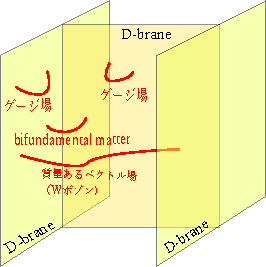
\includegraphics[width=8cm]{generalbrane.pdf}
  \caption{D-braneの配位と、それに端を持つ開弦の例。様々な種類の粒子がD-braneの配位から現れる。}
\end{figure}


\section{境界のある2次元自由スカラー場}

開いた弦は、世界面の理論として、境界のある2次元の場の理論を考えることになります。ここでは、その準備として2次元の1つのスカラー場の理論を考えましょう。

\subsection{作用と境界条件}

空間方向の座標を$\sigma$とし、$0\le \sigma \le \pi$とします。$\sigma=0$と$\sigma=\pi$が境界になります。時間方向の座標を$\tau$とします。

スカラー場を$X(\sigma)$とし、その作用を
\begin{align}
  S=\frac{1}{8\pi}\int \di \tau \int_{0}^{\pi}\di \sigma \left( (\del_{\tau}X)^2-(\del_{\sigma}X)^2 \right)
  \label{actionscalarwithboundary}
\end{align}
とします。

境界がある理論を考えているので、境界条件をどう取るかを考える必要があります。ここでは運動方程式を考えることで、発見法的に境界条件としてどのようなものがあるかを考えます。\eqref{actionscalarwithboundary}の変分をとると
\begin{align}
  \delta S&
  =\frac{1}{4\pi}\int \di \tau \int_{0}^{\pi}\di \sigma \left( \del_{\tau}X\del_{\tau}\delta X - \del_{\sigma}X\del_{\sigma}\delta X \right)\nonumber\\
  &=\frac{1}{4\pi}\int \di \tau \int_{0}^{\pi}\di \sigma \left( (-\del_{\tau}^2X+\del_{\sigma}^2X)\delta X+\del_{\tau}(X\del_{\tau}\delta X) - \del_{\sigma}(X\del_{\sigma}\delta X) \right)
\end{align}
となります。被積分関数の第1項から運動方程式が出ます。第2項は通常の最小作用の原理の設定では、時間の端での境界条件を課すので消えます。第3項が問題でこれを計算すると
\begin{align}
  \delta S = \cdots +\frac{1}{4\pi}\int \di \tau [-\del_{\sigma}X \delta X]_{\sigma=0}^{\pi}
\end{align}
となります。$\delta S=0$となるためには、適切な境界条件を課す必要があります。例えば$\sigma=0$での境界条件を考えてみましょう。$\del_{\sigma}X(0)\delta X(0)=0$となる必要がありますから、例えば次の2つの境界条件があり得ます。
\begin{itemize}
  \item Neumann境界条件(自由端条件)$\del_{\sigma} X(0)=0$. $\sigma=0$で表される弦の端は$X$方向に自由に動くことができるので、「D-braneは$X$方向に伸びている」ということができます。\\
  \begin{center}
    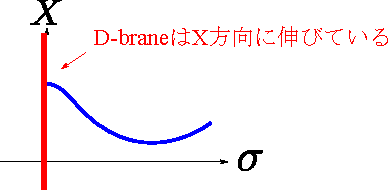
\includegraphics{NBC.pdf}    
  \end{center}
  \item Dirichlet境界条件(固定端条件)$X(0)=v$(定数).$\sigma=0$で表される弦の端は$X=v$のところにしかくっつけないので、「D-braneは$X=v$の場所にある」ということができます。\\
  \begin{center}
    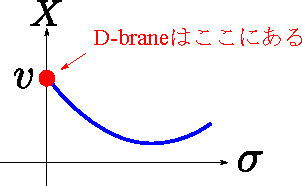
\includegraphics{DBC.pdf}    
  \end{center}
\end{itemize}
同様にして$\sigma=\pi$の方の境界にもNeumann境界条件とDirichlet境界条件の2種類が考えられます。合わせると、$\sigma=0,\pi$の境界条件をNあるいはDで表すことにして、NN, DN, ND, DD の4種類の境界条件のとり方が考えられます。

さて、このような境界条件の場合にエネルギー運動量テンソルがどうなるか見てみましょう。エネルギー運動量テンソルは、以前見たように
\begin{align}
  T_{++}=\frac12 \del_{+}X\del_{+}X,\quad
  T_{--}=\frac12 \del_{-}X\del_{-}X,\quad
  \del_{\pm}:=\frac12 (\del_{\tau}\pm \del_{\sigma})
\end{align}
となります。例えば$\sigma=0$でNeumann境界条件であったとすると$\del_{\sigma}X(0)=0$ですから
\begin{align}
  \del_{+}X(0)=\del_{-}X(0)=\frac12 \del_{\tau}X(0)
\end{align}
となります。したがって$\sigma=0$で$T_{++}=T_{--}$が成り立ちます。一方$\sigma=0$でDirichlet境界条件であったとすると$\del_{\tau}X(0)=0$ですから
\begin{align}
  \del_{+}X(0)=-\del_{-}X(0)=\frac12 \del_{\sigma}X(0)
\end{align}
となります。したがって、やはり$\sigma=0$で$T_{++}=T_{--}$が成り立ちます。まとめるとNeumann境界条件の場合もDirichlet境界条件の場合も境界で
\begin{important}
  \begin{align}
    T_{++}=T_{--}\label{gluingcondition}
  \end{align}
\end{important}
が成り立ちます。ここでは発見法的に境界条件を考えましたが、実は\eqref{gluingcondition}が原理的に境界条件が満たさなければならない条件です。
\eqref{gluingcondition}は境界で$T_{01}=0$と書けます。
これは、エネルギーの流れの境界の垂直方向成分が$0$ということですから、(エネルギーが端に溜まることなく)エネルギーが保存するということと等価です。

\subsection{二重化トリック}
ここでは、境界のある共形場理論の標準的な取り扱いの一つである二重化トリックについて説明します。これは、$0\le \sigma \le \pi$での理論を$0\le \sigma \le 2\pi$で(反)周期的境界条件の場の言葉に書き換える方法です。

エネルギー運動量テンソル$T_{++}(\tau,\sigma),\ (0\le \sigma \le 2\pi)$を次のように定義します。
\begin{align}
  T_{++}(\tau,\sigma):=
  \begin{cases}
    T_{++}(\tau,\sigma)& (0\le \sigma \le \pi)\\
    T_{--}(\tau,2\pi-\sigma) & (\pi\le \sigma \le 2\pi)
  \end{cases}.
\end{align}
このように定義すると、次のような理由で周期境界条件の場合のエネルギー運動量テンソルのうち$T_{++}$だけをとってきたものと同じような性質を満たします。
\begin{itemize}
  \item 境界条件\eqref{gluingcondition}から$T_{++}(\tau,\sigma)$は、$\sigma=\pi$で連続、$T_{++}(\tau,2\pi)=T_{++}(\tau,0)$となります。
  \item $0\le \sigma \le 2\pi$で$\del_{-}T_{++}=0$を満たします。
\end{itemize}
これらの性質からモード展開できて
\begin{align}
  T_{++}(\tau,\sigma)=\sum_{n\in\Zb}
  L_{n}e^{-in\sigma^{+}}
\end{align}
となります。

また、二重化トリックの言葉を用いると古典的なHamiltonianは
\begin{align}
  H=\frac{1}{2\pi}\int_{0}^{\pi}(T_{++}+T_{--})
  =\frac{1}{2\pi}\int_{0}^{2\pi}T_{++}
  =L_{0}
\end{align}
となります。量子化するとc数分ずれる可能性があります。

\subsection{モード展開}
ここから、もっと具体的にスカラー場の運動方程式を解いてモード展開をしていきます。NN, DD, ND, DNの各境界条件をそれぞれ見ていきます。
\subsubsection*{--- NN境界条件 ---}
NN境界条件では、
\begin{align}
  \del_{\sigma}X\Bigg|_{\sigma=0,\pi}=0
\end{align}
となりますから、一般に
\begin{align}
  \del_{\sigma}X(\tau,\sigma)=\sum_{n=1}^{\infty}\At_n(t)\sin n\sigma
\end{align}
と展開することができます。ここから$X(\tau,\sigma)$は
\begin{align}
  X(\tau,\sigma)=A_{0}(\tau)+\sum_{n=1}^{\infty}A_{n}(\tau)\cos n\sigma\label{NNmodes0}
\end{align}
と展開できます。

\eqref{NNmodes0}を運動方程式
\begin{align}
  \del_{\tau}^2X-\del_{\sigma}^2X=0
\end{align}
に代入して整理すると$A_n\ (n=0,1,2,\dots)$に対する方程式
\begin{align}
  \ddot{A}_{n}+n^2 A_n=0
\end{align}
を得ます。$n=0$のときは自由粒子の運動方程式と同じなので$x,p$を定数として一般解を
\begin{align}
  A_{0}(\tau)=x+4p\tau
\end{align}
と書くことができます。$n>0$のときには、調和振動子なので一般解は
\begin{align}
  A_{n}(\tau)=B_{n}e^{-in\tau}+C_{n}e^{in\tau}
\end{align}
となります。積分定数を適当に再定義し、\eqref{NNmodes0}に代入して整理すると
\begin{align}
  X(\tau,\sigma)=x+4p\tau+2i\sum_{n\ne 0}
  \frac{\alpha_{n}}{n}e^{-in\tau}\cos n\sigma
\end{align}
となります。$x,p,\alpha_{n}\ (n\in \Zb, n \ne 0)$が積分定数になります。

量子化しましょう。正準交換関係は、$[X(\sigma),\dot{X}(\sigma')]=4\pi i \delta(\sigma-\sigma')$です。ここから、$x,p,\alpha_{n}$の交換関係は
\begin{align}
  [x,p]=i,\quad [\alpha_{n},\alpha_{m}]=n\delta_{n+m}
\end{align}
となります。これ以外は交換します。

さらに
\begin{align}
  X=x+4p\tau+i\sum_{n\ne 0}\frac{\alpha_{n}}{n}(e^{-in\sigma^{+}}+e^{-in\sigma^{-}})
\end{align}
と書けることに注目すると
\begin{align}
  \del_{+}X=2p+\sum_{n\ne 0}\alpha_{n}e^{-in\sigma^{+}}
  =\sum_{n\in \Zb}\alpha_{n}e^{-in\sigma^{+}}
\end{align}
となります。最後の式では、$\alpha_{0}:=2p$と定義しました。同様にして
\begin{align}
  \del_{-}X=\sum_{n\in \Zb}\alpha_{n}e^{-in\sigma^{-}}
\end{align}
となります。これらは、次のように二重化トリックで$\del_{+}X(\tau,\sigma),\ (0\le \sigma \le 2\pi)$にまとめることができます。
\begin{align}
  \del_{+}X(\tau,\sigma)=
  \begin{cases}
    \del_{+}X(\tau,\sigma)& (0\le \sigma \le \pi)\\
    \del_{-}X(\tau,2\pi-\sigma) & (\pi\le \sigma \le 2\pi)
  \end{cases}.
\end{align}

これを用いると二重化トリックしたエネルギー運動量テンソルは、周期境界条件の場合と同様の計算で
\begin{align}
  T_{++}=\frac12 \del_{+}X\del_{+}X
  =\frac12 \sum_{k}\sum_{m}\alpha_{n}\alpha_{m}e^{-i(k+m)\sigma^{+}}
  =\sum_{n}\frac12\sum_{m}\alpha_{n-m}\alpha_{m}e^{-in\sigma^{+}}
\end{align}
となります。演算子順序によるc数の不定性の部分も周期境界条件の場合と同じで
\begin{align}
  L_{n}=\frac12\sum_{m\in\Zb}\alpha_{n-m}\alpha_{m} \quad (n\ne 0),\quad
  L_{0}=\frac12 \alpha_{0}^2+\sum_{m=1}^{\infty}\alpha_{-m}\alpha_{m}
\end{align}
となります。

真空のエネルギーも周期境界条件の$T_{++}$の方だけの場合と同じで
\begin{align}
  \frac12\sum_{m\in\Zb}\alpha_{-m}\alpha_{m}\Bigg|_{\text{くりこみ}}=L_{0}-\frac{1}{24}
\end{align}
となります。

\subsubsection*{--- DD境界条件 ---}
DD境界条件
\begin{align}
  X(\tau,0)=v_0,\quad X(\tau,\pi)=v_{\pi}
\end{align}
の場合を考えます。この場合
\begin{align}
  X(\tau,\sigma)=v_{0}\left( 1-\frac{\sigma}{\pi} \right)+v_{\pi}\frac{\sigma}{\pi}+\widetilde{X}(\tau,\sigma)
\end{align}
として$\widetilde{X}(\tau,\sigma)$を定義すると
\begin{align}
  \widetilde{X}(\tau,0)=\widetilde{X}(\tau,\pi)=0
\end{align}
となります。したがって
\begin{align}
  \widetilde{X}(\tau,\sigma)=\sum_{n=1}^{\infty}A_{n}(\tau)\sin n\sigma
\end{align}
となります。つまり
\begin{align}
  X(\tau,\sigma)=v_{0}\left( 1-\frac{\sigma}{\pi} \right)+v_{\pi}\frac{\sigma}{\pi}+\sum_{n=1}^{\infty}A_{n}(\tau)\sin n\sigma
\end{align}
となります。これを運動方程式に代入すると
\begin{align}
  \ddot{A}_{n}(\tau)+nA_{n}(\tau)=0 \quad (n=1,2,3,\dots)
\end{align}
という調和振動子の運動方程式になります。その一般解は
\begin{align}
  A_{n}(\tau)=B_{n}e^{-in\tau}+C_{n}e^{in\tau}
\end{align}
となります。定数を再定義して
\begin{align}
  X(\tau,\sigma)=v_{0}+\frac{v_{\pi}-v_{0}}{\pi}\sigma+2\sum_{n\ne 0}^{\infty}\frac{\alpha_{n}}{n}e^{-in\tau}\sin n\sigma
\end{align}
となります。

量子化します。交換関係はこれまでと同じで
\begin{align}
  [\alpha_n,\alpha_m]=n\delta_{n+m}
\end{align}
となります。

また
\begin{align}
  X(\tau,\sigma)=v_{0}+\frac{v_{\pi}-v_{0}}{\pi}\sigma+v_{\pi}\frac{\sigma}{\pi}+i\sum_{n\ne 0}^{\infty}\frac{\alpha_{n}}{n}\left( e^{-in\sigma^{+}}-e^{-in\sigma^{-}} \right)
\end{align}
と書けるので
\begin{align}
  \del_{+}X(\tau,\sigma)=\frac{v_{\pi}-v_{0}}{2\pi}+\sum_{n\ne 0}\alpha_{n}e^{-in\sigma^{+}}=\sum_{n\in \Zb}\alpha_{n}e^{-in\sigma^{+}},\qquad \alpha_{0}:=\frac{v_{\pi}-v_{0}}{2\pi}
  \label{DDmodeexp}
\end{align}
となります。同様に
\begin{align}
  \del_{-}X(\tau,\sigma)=-\sum_{n\in \Zb}\alpha_{n}e^{-in\sigma^{-}}
\end{align}
となります。これらは、次のように二重化トリックで$\del_{+}X(\tau,\sigma),\ (0\le \sigma \le 2\pi)$にまとめることができます。
\begin{align}
  \del_{+}X(\tau,\sigma)=
  \begin{cases}
    \del_{+}X(\tau,\sigma)& (0\le \sigma \le \pi)\\
    -\del_{-}X(\tau,2\pi-\sigma) & (\pi\le \sigma \le 2\pi)
  \end{cases}.
\end{align}
このとき$\del_{+}X(\tau,0)=\del_{+}X(\tau,2\pi)$を満たします。
ここから$T_{++}=\frac12\del_{+}X\del_{+}X=\sum_{n\in \Zb}L_{n}e^{-in\sigma^{+}}$として$L_n$を計算しますが、これは周期境界条件の場合と同じです。
\begin{align}
  L_{n}=\frac12 \sum_{m\in\Zb}\alpha_{n-m}\alpha_{m}\quad (n\ne 0),\quad
  L_{0}=\frac12 \alpha_{0}^2+\sum_{m=1}^{\infty}\alpha_{-m}\alpha_{m}.
\end{align}
真空のエネルギーも同様で
\begin{align}
  \frac12 \sum_{m\in\Zb}\alpha_{n-m}\alpha_{m}\Bigg|_{\text{くりこみ}}=L_0-\frac{1}{24}
\end{align}
となります。


\subsubsection*{--- DN境界条件 ---}
DN境界条件の場合、
\begin{align}
  X(\tau,0)=v_0,\quad \del_{\sigma}X(\tau,\pi)=0
\end{align}
を満たします。このとき$X$は
\begin{align}
  X(\tau,\sigma)=v_0+\sum_{r\in \Zbh,\ r>0}A_{r}(\tau)\sin r\sigma
\end{align}
と展開することができます。これを運動方程式に代入すると、多数の調和振動子になります。これを解くと
\begin{align}
  A_{r}(\tau)=B_{r}e^{-ir\tau}+C_{r}e^{ir\tau}
\end{align}
となります。積分定数を適当に再定義して
\begin{align}
  X(\tau,\sigma)=v_{0}+2\sum_{r\in \Zbh}\frac{\alpha_{r}}{r}e^{-ir\tau}\sin r\sigma
\end{align}
を得ます。モードの交換関係は
\begin{align}
  [\alpha_{r},\alpha_{s}]=r\delta_{r+s}
\end{align}
となります。

微分を計算していきます。
\begin{align}
  &\del_{+}X=\sum_{r\in \Zbh}\alpha_{r}e^{-ir\sigma^{+}},\\
  &\del_{-}X=-\sum_{r\in \Zbh}\alpha_{r}e^{-ir\sigma^{-}}.
\end{align}
となります。これらは、次のように二重化トリックで$\del_{+}X(\tau,\sigma)\ (0\le \sigma \le 2\pi)$にまとめることができます。
\begin{align}
  \del_{+}X(\tau,\sigma)=
  \begin{cases}
    \del_{+}X(\tau,\sigma)& (0\le \sigma \le \pi)\\
    \del_{-}X(\tau,2\pi-\sigma) & (\pi\le \sigma \le 2\pi)
  \end{cases}.
\end{align}
こうすると$\del_{+}X(\tau,0)=-\del_{+}X(\tau,2\pi)$と反周期境界条件になります。

エネルギー運動量テンソルは
\begin{align}
  T_{++}
  =\frac12 \sum_{r,s\in \Zbh}\alpha_{s}\alpha_{r} e^{-i(r+s)\sigma^{+}}
  =\frac12 \sum_{n\in\Zb}\sum_{r\in \Zbh}\alpha_{n-r}\alpha_{r} e^{-in\sigma^{+}}
\end{align}
となりますから、
\begin{align}
  L_{n}=\frac12 \sum_{r\in \Zbh}
  \alpha_{n-r}\alpha_{r}\quad (n\ne 0),\quad
  L_{0}=\sum_{r\in \Zbh,r>0}\alpha_{-r}\alpha_{r}+b
\end{align}
となります。$b$はこれから決めるc数です。

$b$を決めましょう。これは、Virasoro代数の一部
\begin{align}
  [L_{1},L_{-1}]=2L_0
\end{align}
が成り立つように決めます。Fock真空を$\ket{0},\ \alpha_{r}\ket{0}=0\ (r>0),\ \braket{0}{0}=1$として、ここから
\begin{align}
  2b
  &=\bra{0}[L_{1},L_{-1}]\ket{0}
  =\bra{0}L_{1}L_{-1}\ket{0}
  =\sum_{r,s}\frac14\bra{0}\alpha_{1-s}\alpha_{s}\alpha_{-1-r}\alpha_{r}\ket{0}\nonumber\\
  &
  =\frac14\bra{0}\alpha_{\frac12}\alpha_{\frac12}\alpha_{-\frac12}\alpha_{-\frac12}\ket{0}
  =\frac14\bra{0}\alpha_{\frac12}\alpha_{-\frac12}\alpha_{\frac12}\alpha_{-\frac12}\ket{0}
  +\frac18\bra{0}\alpha_{\frac12}\alpha_{-\frac12}\ket{0}
  =\frac18
\end{align}
となるので
\begin{align}
  b=\frac{1}{16}
\end{align}
を得ます。しがたって
\begin{align}
  L_{0}=\sum_{r\in \Zbh,r>0}\alpha_{-r}\alpha_{r}+\frac{1}{16}
\end{align}
となります。真空のエネルギーは
\begin{align}
  \frac12 \sum_{r\in \Zbh}\alpha_{-r}\alpha_{r}\Bigg|_{\text{くりこみ}}
  =
  \sum_{r\in \Zbh,\ r>0}\alpha_{-r}\alpha_{r}
  +\frac12 \sum_{r\in \Zbh,\ r>0}r\Bigg|_{\text{くりこみ}}
  =
  \sum_{r\in \Zbh,\ r>0}\alpha_{-r}\alpha_{r}
  +\frac{1}{48}
\end{align}
となります。ここでは、\eqref{zetafunction}と\eqref{zetavalue}から$\zeta(-1,\frac12)=\frac{1}{24}$であることを用いました。

\subsubsection*{--- ND境界条件 ---}
ND境界条件の場合、
\begin{align}
  \del_{\sigma}X(\tau,0)=0,\quad X(\tau,\pi)=v_{\pi}
\end{align}
を満たします。これは、DN境界条件の場合とほぼ同様に考えることができます。
このとき$X$は
\begin{align}
  X(\tau,\sigma)=v_{\pi}+\sum_{r\in \Zbh,\ r>0}A_{r}(\tau)\cos r\sigma
\end{align}
と展開することができます。これを運動方程式に代入すると、多数の調和振動子になります。これを解くと
\begin{align}
  A_{r}(\tau)=B_{r}e^{-ir\tau}+C_{r}e^{ir\tau}
\end{align}
となります。積分定数を適当に再定義して
\begin{align}
  X(\tau,\sigma)=v_{\pi}+2i\sum_{r\in \Zbh}\frac{\alpha_{r}}{r}e^{-ir\tau}\cos r\sigma
\end{align}
を得ます。モードの交換関係は
\begin{align}
  [\alpha_{r},\alpha_{s}]=r\delta_{r+s}
\end{align}
となります。

微分を計算していきます。
\begin{align}
  &\del_{+}X=\sum_{r\in \Zbh}\alpha_{r}e^{-ir\sigma^{+}},\\
  &\del_{-}X=\sum_{r\in \Zbh}\alpha_{r}e^{-ir\sigma^{-}}.
\end{align}
となります。これらは、次のように二重化トリックで$\del_{+}X(\tau,\sigma),\ (0\le \sigma \le 2\pi)$にまとめることができます。
\begin{align}
  \del_{+}X(\tau,\sigma)=
  \begin{cases}
    \del_{+}X(\tau,\sigma)& (0\le \sigma \le \pi)\\
    -\del_{-}X(\tau,2\pi-\sigma) & (\pi\le \sigma \le 2\pi)
  \end{cases}.
\end{align}
こうすると$\del_{+}X(\tau,0)=-\del_{+}X(\tau,2\pi)$と反周期境界条件になります。

エネルギー運動量テンソルは
\begin{align}
  T_{++}
  =\frac12 \sum_{r,s\in \Zbh}\alpha_{s}\alpha_{r} e^{-i(r+s)\sigma^{+}}
  =\frac12 \sum_{n\in\Zb}\sum_{r\in \Zbh}\alpha_{n-r}\alpha_{r} e^{-in\sigma^{+}}
\end{align}
となりますから、
\begin{align}
  L_{n}=\frac12 \sum_{r\in \Zbh}
  \alpha_{n-r}\alpha_{r},\quad (n\ne 0),\quad
  L_{0}=\sum_{r\in \Zbh,r>0}\alpha_{-r}\alpha_{r}+\frac{1}{16}
\end{align}
となります。$L_0$の定数部分はDNの場合と全く同じ計算になるので$\frac{1}{16}$です。

真空のエネルギーもDNの場合と全く同じで
\begin{align}
  \frac12 \sum_{r\in \Zbh}\alpha_{-r}\alpha_{r}\Bigg|_{\text{くりこみ}}
  =
  \sum_{r\in \Zbh,\ r>0}\alpha_{-r}\alpha_{r}
  +\frac{1}{48}
\end{align}
となります。

\section{ボゾン的弦理論のD-brane}
さて、2次元の境界付きの自由スカラー場の理論の準備は終えたので、実際に弦理論におけるD-braneの解析を進めましょう。

\subsection{1枚の平らなD-brane}
まずは、一番簡単なところで26次元時空にある、1枚の平らなD-braneを考えます(図\ref{fig:singlebrane}参照)。この系では、閉じた弦の他に、D-braneにくっついている開弦があります。この開弦を調べることにより、D-braneがあることによる余分な励起にどのようなものがあるかを調べることが出来ます。
\begin{figure}
  \centering
  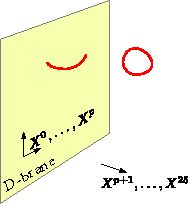
\includegraphics[scale=1.5]{singlebrane.pdf}
  \caption{1枚のD$p$-brane。閉弦に加えて、D-braneに端を持つ開弦が励起として存在します。}
  \label{fig:singlebrane}
\end{figure}


この平らなD-braneは$X^0,\dots,X^{p}$方向にのびていて、$X^{p+1},\dots,X^{25}$方向には局在しているとします。このように空間方向$p$次元にのびているD-braneをD$p$-braneと呼びます。ここにくっついている開弦の世界面の場の理論においては
\begin{itemize}
  \item $X^0,\dots,X^{p}$がNN境界条件。
  \item $X^{p+1},\dots,X^{25}$がDD境界条件。
\end{itemize}
になります。この講義では光円錐ゲージを考えたいので、$p\ge 1$の場合を考えます。

さて光円錐ゲージを考えましょう。閉弦の場合と同様に
\begin{align}
  X^{\pm}:=\frac{1}{\sqrt{2}}(X^{0}\pm X^{1})
\end{align}
として、ゲージ固定条件
\begin{align}
  X^{+}(\tau,\sigma)=4p^{+}\tau
\end{align}
を課します。こうすると拘束条件
\begin{align}
  T_{++}(\tau,\sigma)-a=0
\end{align}
を解くことができて
\begin{align}
  \del_{+}X^{-}=\frac{1}{2p^{+}}\left( \frac12 \del_{+}X^{i}\del_{+}X^{i}-a \right),\quad i=2,\dots,26
\end{align}
となります。今、$a$は、NN, DD方向からの寄与が$\frac{1}{24}$ですから、$a=1$となります。このゼロモードを考えると
\begin{align}
  \alpha^{-}_{0}=\frac{1}{2p^{+}}\left( \frac12 \alpha_{0}^{\ell}\alpha_{0}^{\ell}+N-1 \right),\quad N:=\sum_{n=1}^{\infty} \alpha_{-n}^{i}\alpha_{n}^{i},\quad \ell=2,\dots,p\label{singlebranezeromode}
\end{align}
となります。ここで、DD境界条件のボゾンのゼロモードは\eqref{DDmodeexp}のように表され、しかも今は1枚しかD-braneがないので$v_0=v_{\pi}$となり、ゼロモードは消えることを用いました。要するに、D-braneの伸びていない方向には開弦は運動量を持てないということです。$\alpha^{\mu}_{0}=2p^{\mu}$であることを考慮すると$(p+1)$次元の意味での質量$m^2$は
\begin{align}
  m^2:=2p^{+}p^{-}-p^{\ell}p^{\ell}=\frac{N-1}{2}\label{massopen1Dp}
\end{align}
となります。

さて、スペクトルを調べていきましょう。まず、Fock真空$\ket{k}$は
\begin{align}
  p^{+}\ket{k}=k^{+}\ket{k},\quad
  p^{\ell}\ket{k}=k^{\ell}\ket{k}\ (\ell=2,\dots,p),\nonumber\\
 \alpha_{n}^{i}\ket{k}=0\ (n>0,\ i=2,\dots,25)
\end{align}
という状態です。これは$N=0$であり\eqref{massopen1Dp}より$m^2=-\frac12$となるのでタキオンになります。

次に第1励起状態を見てみましょう。この状態は
\begin{align}
  \alpha_{-1}^{\ell}\ket{k},\quad 
  \alpha_{-1}^{j}\ket{k}\ (j=p+1,\dots,25)
\end{align}
です。この状態は$N=1$なので質量は\eqref{massopen1Dp}より$m^2=0$となって無質量状態となります。これらの無質量の場は両方とも重要な意味があります。
\begin{itemize}
  \item $\alpha_{-1}^{\ell}\ket{k}$は、$(p+1)$次元のLorentz群のうち、あらわに見えているSO$(p-1)$に対してベクトル表現になっています。ですから、$(p+1)$次元のベクトル粒子になります。これは、このD-braneの上にU(1)ゲージ対称性があることを示します。
  \item $\alpha_{-1}^{j}\ket{k}$は$(p+1)$次元のスカラー粒子になります。また、$(p+1)$次元の言葉で言うと内部対称性である、D-braneに垂直方向の回転SO$(25-p)$のベクトル表現になっています。今考えている系はD-braneの存在により、時空の並進対称性を一部破っています。$\alpha_{-1}^{j}\ket{k}$のスカラー粒子の対称性に対する変換性を考えると、これらが並進対称性の自発的破れによるNGボゾンであることが分かります。言い換えると、このスカラー場はD-braneの垂直方向のゆらぎを表します。
\end{itemize}

\subsection{2枚の並行なD-brane}
次に2枚の平行なD$p$-braneを考えます(図\ref{fig:parallelbrane}参照)。2つのbraneは$X^{25}$方向のみに離れていて、座標はそれぞれ$X^{25}=0$、$X^{25}=v$とします。この系では、閉弦、それぞれの片方のD-braneにくっついている開弦に加えて、2つのD-braneをつなぐ開弦が励起としてあります。
\begin{figure}
  \centering
  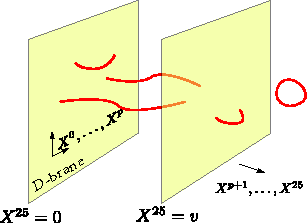
\includegraphics[scale=1.5]{parallelbrane.pdf}
  \caption{2枚の並行なD$p$-brane。}
  \label{fig:parallelbrane}
\end{figure}

片方のD-braneだけにくっついている開弦は前項で調べたので、ここでは2つのbraneをつなぐ開弦を考えましょう。この場合やはり
\begin{itemize}
  \item $X^0,\dots,X^{p}$がNN境界条件。
  \item $X^0,\dots,X^{p}$がDD境界条件。
\end{itemize}
となります。なので、ほとんど前項の解析と同様にできます。前項の解析との違いは、DD方向のうち$X^{25}$のゼロモードが$0$にならないことです。したがって、光円錐ゲージで拘束条件を解いたとき\eqref{singlebranezeromode}が変更されて
\begin{align}
  \alpha^{-}_{0}=\frac{1}{2p^{+}}\left( \frac12 \alpha_{0}^{\ell}\alpha_{0}^{\ell}+\frac12 \alpha_{0}^{25}\alpha_{0}^{25}+N-1 \right),\quad N:=\sum_{n=1}^{\infty} \alpha_{-n}^{i}\alpha_{n}^{i},\quad \alpha_{0}^{25}=\frac{v}{2\pi}
\end{align}
となります。したがって、$(p+1)$次元の意味での質量は
\begin{align}
  m^2=\left( \frac{v}{4\pi} \right)^2+\frac12(N-1)
\end{align}
となります。

スペクトルを調べましょう。Fock真空$\ket{k}$は$N=0$ですから、その質量は$m^2=\left( \frac{v}{4\pi} \right)^2-1$となります。これは、$v$が小さいときにはタキオンですが、ある程度大きくなると有質量になります。

第1励起状態は、$\alpha_{-1}^{\ell}\ket{k}\  (\ell=2,\dots,p),\ 
\alpha_{-1}^{j}\ket{k}\ (j=p+1,\dots,25)$です。その質量は
\begin{align}
  m^2=\left( \frac{v}{4\pi} \right)^2
\end{align}
ですから$v\ne 0$のときには有質量になります。$\alpha_{-1}^{\ell}\ket{k}$はSO$(p-1)$のベクトルになります。$(p+1)$次元の有質量ベクトル粒子の一部になります。$(p+1)$次元の有質量ベクトル粒子の偏光は$p$個ありますから、$\alpha_{-1}^{\ell}\ket{k}$以外にもう一つこのベクトル粒子の偏光になっているものがあります。これはSO$(p-1)$のスカラーである$\alpha_{-1}^{25}\ket{k}$です。それ以外のスカラー$\alpha_{-1}^{j}\ket{k}\ (j=p+1,\dots,24)$は、$(p+1)$次元のスカラー粒子になっています。

さて、開弦のスペクトルについてまとめておきましょう。そのために2つのD-braneに①、②というラベルをふります。そして例えば①と②をつなぐ弦を①②弦などと呼ぶことにします。①①弦から①のD-brane上にU(1)ゲージ場ができます。このU(1)対称性をU$(1)_1$と呼ぶことにします。同様に②②弦によって作られるゲージ場のU(1)対称性をU$(1)_2$と呼ぶことにします。①②弦や②①弦はこれらのU(1)対称性について電荷を持つことになります。これらの電荷について表にまとめておきます。
\begin{table}
  \centering
  \begin{tabular}{|c|c|c|}\hline
    & U$(1)_1$電荷 & U$(1)_2$電荷\\ \hline
    ①①弦無質量ベクトル、スカラー & 0 & 0 \\ \hline
    ②②弦無質量ベクトル、スカラー & 0 & 0 \\ \hline
    ①②弦有質量ベクトル、スカラー & $+1$ & $-1$ \\ \hline
    ②①弦有質量ベクトル、スカラー & $-1$ & $+1$ \\ \hline
  \end{tabular}
  \caption{平行な2枚のD-braneの各種開弦の電荷}
  \label{tab:charges}
\end{table}

ここで、$v\to 0$とした場合に何がおこるかを考えてみましょう。それまで有質量だった①②弦と②①弦から出てくるベクトル場やスカラー場が無質量になります。これに伴い、ゲージ対称性が拡大します。表\ref{tab:charges}も考え合わせると、拡大された対称性はU$(2)$になります。スカラー場は、随伴表現になります。こうして、非可換なゲージ対称性が現れることになります。$v\ne 0$は、この随伴表現のスカラー場が真空期待値を持つことを意味します。この真空期待値によりゲージ対称性がU$(2)$から自発的に敗れてU$(1)\times $U$(1)$になり、一部のゲージ場が有質量になります。つまりHiggs機構を起こすのです。

ここで少し不思議なのは、2つのD-braneの位置は2つの数(あるいは、垂直方向の2つのベクトル)だったのですが、U$(2)$が回復する点では、$2\times 2$の行列(からなるベクトル)になります。これは、古典的には非常に想像しにくい場の理論、あるいは弦理論独特の現象です。

同様にして$n$枚の重なったD-braneがあるときには、U$(n)$のゲージ対称性が現れます。そこには随伴表現の無質量スカラー場があり、これが真空期待値をとることにより一般にはU$(1)^n$に自発的に破れます。

\subsection{2つの異なるD-brane}

次に次元が異なる2つのD-braneを考えます。図\ref{fig:ppprimebrane}を見てください。$p'>p$としてD$p$-braneとD$p'$-braneを考え、D$p$-braneの方は$X^{0},\dots,X^{p}$の方向に伸びており、D$p'$-braneの方は$X^{0},\dots,X^{p'}$の方に伸びているとします。

\begin{figure}
  \centering
  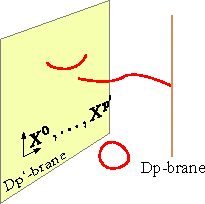
\includegraphics[scale=1.5]{ppprimebrane.pdf}
  \caption{次元が異なる2つのD-brane}
  \label{fig:ppprimebrane}
\end{figure}

それぞれのD-braneにくっついている開弦はもうやりました。これらは、それぞれのD-braneの上にU$(1)$ゲージ場をつくります。さらにD$p$-braneとD$p'$-braneにくっついている開弦は、D$p$-braneのゲージ場に対して、その向きによって電荷が$+1$または$-1$になります。もし、D$p'$-braneが$N_f$枚あったとすると、それはD$p$-braneの上から見れば$N_f$個のフレーバーに見えます。

さらにD$p$-braneとD$p'$-braneにくっついている開弦のスペクトルについて考えてみましょう。境界条件は
\begin{itemize}
  \item $X^{0},\dots,X^{p}$: NN.
  \item $X^{p+1},\dots,X^{p'}$: ND, DN.
  \item $X^{p'+1},\dots,X^{25}$: DD.
\end{itemize}
となります。質量は、brane間の距離を$v$として
\begin{align}
  m^{2}=\left( \frac{v}{4\pi} \right)^2+\frac12\left( N-1+\frac{p'-p}{16} \right)
\end{align}
となります。これは、$v=0,\ N=1$でも有質量であることに注意してください。

\section{2次元超対称理論の境界}
次に超弦理論での弦理論を考えたいです。そのために、ここではまず超対称性のある2次元の理論の境界について調べましょう。

\subsection{超対称性のカレントに対する境界条件}
超弦理論に使うためには超対称性が保存するような境界条件を課す必要があります。

ここで考える理論の作用を
\begin{align}
  S=\frac{1}{2\pi}\int d^2\sigma \left( 
    \del_{+}X \del_{-} X+i\psi_{+}\del_{-}\psi_{+}+i\psi_{-}\del_{+}\psi_{-}
   \right),\quad 0\le \sigma \le \pi
\end{align}
とします。超対称性のカレントは
\begin{align}
  G_{++}=\psi_{+}\del_{+}X,\quad
  G_{--}=\psi_{-}\del_{-}X  
\end{align}
です。

境界で超対称性を保存するためには$\sigma=0,\pi$で
\begin{align}
  G_{++}=\pm G_{--}\label{Gboundarycondition0}
\end{align}
を満たす必要があります。カイラルなフェルミオン数の対称性$\psi_{-}\to \psi_{-}$がありますから、\eqref{Gboundarycondition0}で$-$符号の方も許されることに注意してください。この対称性を利用して$\sigma=\pi$で
\begin{align}
  G_{++}=G_{--}
\end{align}
とします。そうすると、超対称性を保つ境界条件には$\sigma=0$で
\begin{itemize}
  \item $G_{++}=-G_{--}$: NSセクター
  \item $G_{++}=G_{--}$: Rセクター
\end{itemize}
の2種類があります。

\subsection{二重化のトリック}
超対称性のカレントに対する二重化のトリックを考えます。$G_{++}(\tau,\sigma)\ (0\le \sigma \le 2\pi)$を次のように定義します。
\begin{align}
  G_{++}(\tau,\sigma)
  =
  \begin{cases}
    G_{++}(\tau,\sigma) & (0\le \sigma \le \pi)\\
    G_{--}(\tau,2\pi-\sigma) & (\pi\le \sigma \le 2\pi)
  \end{cases}.
\end{align}
こうすると$\sigma=\pi$で連続になります。さらに
\begin{itemize}
  \item $G_{++}(\tau,2\pi)=-G_{++}(\tau,0)$: NSセクター
  \item $G_{++}(\tau,2\pi)=G_{++}(\tau,0)$: Rセクター
\end{itemize}
という(反)周期境界条件を満たします。また$\del_{-}G_{++}=0$を満たしますから$G_{++}$は$\sigma^{+}$だけによっており
\begin{align}
  G_{++}(\tau,\sigma)=\sum_{r}G_{r}e^{-ir\sigma^{+}},\quad
  \begin{cases}
    r\in \Zbh & (\text{NSセクター})\\
    r\in \Zb & (\text{Rセクター})
  \end{cases}
\end{align}
とモード展開できます。

\subsection{フェルミオンの境界条件}
さて、ここでは、ボゾンのNN, DD, ND, DNの各境界条件に対して、具体的にフェルミオンに対する境界条件を求めてみることにします。

\subsubsection*{--- NN境界条件 ---}
$\sigma=\pi$では、$\del_{+}X=\del_{-}X$です。$G_{++}=G_{--}$ですから
$\psi_{+}=\psi_{-}$
となります。

$\sigma=0$では、$\del_{+}X=\del_{-}X$です。
\begin{itemize}
  \item NSセクター: $G_{++}=-G_{--}\ \Rightarrow\ 
  \psi_{+}=-\psi_{-}$
  \item Rセクター: $G_{++}=G_{--}\ \Rightarrow\ 
  \psi_{+}=\psi_{-}$
\end{itemize}
となります。

二重化のトリックを用いると$\psi_{+}(\tau,\sigma)\ (0\le \sigma \le 2\pi)$が定義できて
\begin{itemize}
  \item NSセクター: $\psi_{+}(\tau,2\pi)=-\psi_{+}(\tau,0)$で反周期的。
  \item Rセクター: $\psi_{+}(\tau,2\pi)=\psi_{+}(\tau,0)$で周期的。
\end{itemize}
となります。反周期的、周期的なフェルミオンは\ref{sec:fermion}節での取り扱いと同じです。

\subsubsection*{--- DD境界条件 ---}
$\sigma=\pi$では、$\del_{+}X=-\del_{-}X$です。$G_{++}=G_{--}$ですから
$\psi_{+}=-\psi_{-}$
となります。

$\sigma=0$では、$\del_{+}X=-\del_{-}X$です。
\begin{itemize}
  \item NSセクター: $G_{++}=-G_{--}\ \Rightarrow\ 
  \psi_{+}=\psi_{-}$
  \item Rセクター: $G_{++}=G_{--}\ \Rightarrow\ 
  \psi_{+}=-\psi_{-}$
\end{itemize}
となります。

二重化のトリックを用いると$\psi_{+}(\tau,\sigma)\ (0\le \sigma \le 2\pi)$が定義できて
\begin{itemize}
  \item NSセクター: $\psi_{+}(\tau,2\pi)=-\psi_{+}(\tau,0)$で反周期的。
  \item Rセクター: $\psi_{+}(\tau,2\pi)=\psi_{+}(\tau,0)$で周期的。
\end{itemize}
となります。

\subsubsection*{--- DN境界条件 ---}
$\sigma=\pi$では、$\del_{+}X=\del_{-}X$です。$G_{++}=G_{--}$ですから
$\psi_{+}=\psi_{-}$
となります。

$\sigma=0$では、$\del_{+}X=-\del_{-}X$です。
\begin{itemize}
  \item NSセクター: $G_{++}=-G_{--}\ \Rightarrow\ 
  \psi_{+}=\psi_{-}$
  \item Rセクター: $G_{++}=G_{--}\ \Rightarrow\ 
  \psi_{+}=-\psi_{-}$
\end{itemize}
となります。

二重化のトリックを用いると$\psi_{+}(\tau,\sigma)\ (0\le \sigma \le 2\pi)$が定義できて
\begin{itemize}
  \item NSセクター: $\psi_{+}(\tau,2\pi)=\psi_{+}(\tau,0)$で周期的。
  \item Rセクター: $\psi_{+}(\tau,2\pi)=-\psi_{+}(\tau,0)$で反周期的。
\end{itemize}
となります。


\subsubsection*{--- ND境界条件 ---}
$\sigma=\pi$では、$\del_{+}X=-\del_{-}X$です。$G_{++}=G_{--}$ですから
$\psi_{+}=-\psi_{-}$
となります。

$\sigma=0$では、$\del_{+}X=\del_{-}X$です。
\begin{itemize}
  \item NSセクター: $G_{++}=-G_{--}\ \Rightarrow\ 
  \psi_{+}=-\psi_{-}$
  \item Rセクター: $G_{++}=G_{--}\ \Rightarrow\ 
  \psi_{+}=\psi_{-}$
\end{itemize}
となります。

二重化のトリックを用いると$\psi_{+}(\tau,\sigma)\ (0\le \sigma \le 2\pi)$が定義できて
\begin{itemize}
  \item NSセクター: $\psi_{+}(\tau,2\pi)=\psi_{+}(\tau,0)$で周期的。
  \item Rセクター: $\psi_{+}(\tau,2\pi)=-\psi_{+}(\tau,0)$で反周期的。
\end{itemize}
となります。


\subsection{真空のエネルギー}
これらの結果をまとめて、真空のエネルギー($a$と書いていたもの)をまとめておきます。

まず、表\ref{tab:bosonfermiona}に、(反)周期的なボゾン、フェルミオンの$a$の値をまとめておきます。
\begin{table}
  \centering
  \begin{tabular}{|c||c|c|}\hline
    & 周期的 & 反周期的 \\ \hline\hline
  ボゾン & $\frac{1}{24}$ & $-\frac{1}{48}$\\ \hline
  フェルミオン & $-\frac{1}{24}$&  $\frac{1}{48}$\\ \hline
  \end{tabular}
  \caption{$a$の値の表。ボゾンかフェルミオンか、二重化のトリックをしたときに周期的か反周期的かによる。}
  \label{tab:bosonfermiona}
\end{table}

これらから、各境界条件に対する$a$の値は次のようになります。
\begin{itemize}
  \item NN, DD: 
  \begin{align}
    \text{NSセクター:}& \frac{1}{24}+\frac{1}{48}=\frac{1}{16}, \nonumber\\
    \text{Rセクター:}& \frac{1}{24}-\frac{1}{24}=\frac{1}{16}. \nonumber\\
  \end{align} 
  \item ND, DN: 
  \begin{align}
    \text{NSセクター:}& -\frac{1}{48}-\frac{1}{24}=-\frac{1}{16}, \nonumber\\
    \text{Rセクター:}& -\frac{1}{48}+\frac{1}{48}=0. \nonumber\\
  \end{align} 
\end{itemize}
これを見るとRセクターはいつも$0$、NSセクターはNN, DDに比べてND, DNは$\frac18$だけ小さいことが分かります。

\section{超弦理論のD-brane}
ここでは超弦理論のD-braneを調べていきます。

\subsection{1枚のD-brane}
まず、1枚のD-braneを調べます。空間$p$次元にのびているD$p$-braneを考えます。$X^{0},\dots,X^{p}$の方向にのびているとします。

このD-braneに両端をもつ開弦を考えます。この開弦の境界条件は次のようになります。
\begin{itemize}
  \item $X^{0},\dots,X^{p}$はNN境界条件。
  \item $X^{p+1},\dots,X^{9}$はDD境界条件。
\end{itemize}
二重化のトリックをするとボゾンは全て周期的になります。フェルミオンは全てNSセクターでは反周期的、Rセクターでは周期的になります。

光円錐ゲージをとって考えます。ゲージ固定条件は
\begin{align}
  X^{+}=4p^{+}\tau,\quad \psi_{+}^{+}=0
\end{align}
とします。これを用いて拘束条件
\begin{align}
  T_{++}=0,\quad G_{++}=0
\end{align}
を解くことができます。特に$p+1$次元の意味での質量が求まって
\begin{align}
  &m^2:=2p^{+}p^{-}-p^{\ell}p^{\ell}=\frac{N-a}{2}\quad (\ell=2,\dots,p),\\ 
  &N:=\sum_{n=1}^{\infty}\alpha_{-n}^{i}\alpha_{n}^{i}+\sum_{r>0}r\psi_{-r}^{i}\psi_{r}^{i}\quad (i=2,\dots,9)
\end{align}
となります。ここで、NSセクターでは$a=\frac12$、Rセクターでは$a=0$となります。

スペクトルを調べていくことにしましょう。まずNSセクターのFock真空$\ket{k}$は、$m^2=-\frac14$となり、タキオンになります。この状態は、場合によってはGSO射影で消えます。開弦の場合にGSO射影をどう課すべきかについては、この講義では詳しくは話せませんが、結果の一部だけを説明します。この講義では、このタキオン状態がGSO射影で消せる場合のみを考えます。

NSセクターの第1励起状態は$N=\frac12$で$m^2=0$となります。タキオンがGSO射影で消える場合には、この状態は残ります。次の2種類の状態があります。
\begin{itemize}
  \item $\psi_{-\frac12}^{\ell}$: これは、SO$(p-1)$のベクトル表現になります。したがって$p+1$次元の意味での質量のないベクトル粒子になり、D-brane上のU$(1)$ゲージ場になります。
  \item $\psi_{-\frac12}^{j}\ (j=p+1,\dots,9)$: これは、SO$(p-1)$のスカラーになり、SO$(9-p)$のベクトル表現になります。したがって$p+1$次元の意味での質量のないスカラー粒子になり、D-braneの垂直方向のゆらぎを表すスカラー場になります。
\end{itemize}

RセクターのFock真空は$N=0$で$m^2=0$となります。ゼロモード$\psi^{i}_{0}$があるので、SO$(p-1)$のスピノール表現でSO$(9-p)$のスピノール表現でもあります。GSO射影により、8成分残ります。

もし上で述べたようなGSO射影が出来るとすると、時空の超対称性が存在します。例えば、同じ質量ごとにNSセクターの状態の数とRセクターの状態の数が等しくなります。このようなD-braneを\kyou{BPS D-brane}と呼びます。

どのようなBPS D-braneが存在するかは、type IIBかtype IIAかによって異なります。
\begin{itemize}
  \item Type IIBではBPS D$p$-brane($p$は奇数)が存在します。
  \item Type IIAではBPS D$p$-brane($p$は偶数)が存在します。
\end{itemize}
どうしてこうなるかは、この講義の範囲内では説明できません。

上で求めたBPS D-brane上の無質量のスペクトルは、まとめると10次元の超対称U$(1)$ゲージ理論を$p+1$次元に次元削減したものになります。

$n$枚重なったD$p$-braneを考えるとU$(n)$ゲージ対称性が現れます。例えばtype IIBのD3-braneを考えた場合、brane上の無質量の場は4次元の$\mathcal{N}=4$超対称Yang-Mills理論の場と同じになります。ここで低エネルギー極限をとると閉弦が結合しなくなり、4次元だけの理論になります。4次元で$\mathcal{N}=4$超対称性を持ち、重力の入っていない場の理論は$\mathcal{N}=4$超対称Yang-Mills理論のみで、これはゲージ群と結合定数と$\theta$角を決めると一意に決まると考えられています。D3-braneの低エネルギー理論は、ゲージ群はU$(n)$と分かっています。また、結合定数と$\theta$角は、閉弦から来る場の真空期待値と対応づけることができるので、低エネルギーでの理論が完全に決まることになります。

\subsection{D-braneの系}

次に様々なD-braneの系を考えることにします。

一つのD-braneに両端を持つ開弦はもうすでに考えました。異なるD-braneに端を一つずつもつ開弦を考えます。
この開弦で$q$個のDN, ND方向があり、その他の$10-q$個の方向がNNあるいはDDの場合を考えます。このとき、「時空の超対称性を保つか?」ということを考えます。
このために真空のエネルギーを考えてみましょう。Rセクターでは、いつも$a=0$です。NSセクターでは、
\begin{align}
  a=\frac12-\frac18 q\label{susyaNS}
\end{align}
となります。モードは最小でエネルギーを$\frac12$変えますから、もし\eqref{susyaNS}が$\frac12$の倍数でなければ、RセクターとNSセクターのエネルギーが同じになることはありません。したがって時空の超対称性はないことになります。つまり
\begin{important}
  $q=0,4,8$のいずれかであることが、時空の超対称性があることの必要条件である。
\end{important}
ということができます。

\begin{table}
  \centering
  \begin{tabular}{|c||c|c|c|c|c|c|c|c|c|c|}\hline
    &0 &1 &2 &3 &4 &5 &6 &7 &8 &9 \\ \hline\hline
  D3&○&○&○&○&×&×&×&×&×&×\\ \hline    
  D7&○&○&○&○&○&○&○&○&×&×\\ \hline    
  \end{tabular}
  \caption{D3-braneとD7-braneの系。○がD-braneが伸びている方向。×がD-braneが伸びていない方向。}
  \label{tab:D3D7}
\end{table}
$q=4$の例として、表\ref{tab:D3D7}のようなtype IIB超弦理論でのD3-braneとD7-braneの配位を考えます。この場合、D3-D7をつなぐ弦では、NSセクター、Rセクターともに$a=0$となります。したがって質量はD3-braneとD7-braneの間の距離を$v$として
\begin{align}
  m^2=\left( \frac{v}{4\pi} \right)^2+N
\end{align}
となります。$N=0$の状態を詳しく調べましょう。
\begin{itemize}
  \item NSセクターでは$\psi_{+}^{4},\psi_{+}^{5},\psi_{+}^{6},\psi_{+}^{7}$にゼロモードがあります。これは$\psi_{0}^{4},\psi_{0}^{5},\psi_{0}^{6},\psi_{0}^{7}$で、SO$(4)$のClifford代数をなします。つまり、$X^{4},\dots,X^{7}$を回転するSO$(4)$=SU$(2)\times$SU$(2)$のDiracスピノール表現$(\mathbf{2},\mathbf{1})\oplus(\mathbf{1},\mathbf{2})$になります。GSO射影によってWeylスピノール表現$(\mathbf{2},\mathbf{1})$になります。
  \item Rセクターでは、$\psi_{+}^{2},\psi_{+}^{3},\psi_{+}^{7},\psi_{+}^{8}$にゼロモード$\psi_{0}^{2},\psi_{0}^{3},\psi_{0}^{7},\psi_{0}^{8}$があります。このために4つの状態があります。GSO射影によって2つの状態になります。
\end{itemize}
向きを反対にしたD7-D3弦と合わせて、これらの状態は4次元の$\Ncal=2$超対称性のハイパー多重項というまとまりを作ります。特に$n$枚のD3-braneと$N_f$枚のD7-braneを考えた場合には、4次元で比較的軽い場は
\begin{itemize}
  \item 4次元$\Ncal=4$ U$(n)$ 超対称Yang-Mills理論。
  \item $N_f$個の基本表現のハイパー多重項。
\end{itemize}
となります。

\begin{table}
  \centering
  \begin{tabular}{|c||c|c|c|c|c|c|c|c|c|c|}\hline
    &0 &1 &2 &3 &4 &5 &6 &7 &8 &9 \\ \hline\hline
  D4&○&○&○&○&○&×&×&×&×&×\\ \hline    
  D6&○&○&×&×&×&○&○&○&○&○\\ \hline    
  \end{tabular}
  \caption{D4-braneとD6-braneの系。}
  \label{tab:D4D6}
\end{table}
$q=8$の例として、表\ref{tab:D4D6}のようなtype IIA超弦理論でのD4-braneとD6-braneの配位を考えます。この場合、D4-D6をつなぐ弦で比較的軽い状態を調べてみましょう。NSセクターでは、$a=\frac12$となるのでFock真空は$m^2=\frac14$となって有質量になります。Rセクターは$a=0$ですので$m^2=0$です。今、質量とは2次元のPoincar\'e対称性に対する質量ですので、$p^{+}p^{-}=0$となります。$p^{+}=0$の場合には光円錐ゲージで考えることは出来ませんので、ここでは、$p^{-}=0$の場合を考えます。これはフェルミオンで$X^{1}$の正の方向に光の速さで走っていることになります。つまり2次元の意味でのカイラル・フェルミオンを表します。

現実の世界を記述するためには、カイラル・フェルミオンを含むことが必須です。上のD4-D6の系は非常に簡単で2次元ですが、弦理論がカイラル・フェルミオンを含むことが出来るということの例になっています。

\section{まとめ}
この章ではD-braneについて考えてきました。
\begin{itemize}
  \item D-braneとは弦理論において開弦がくっつくことができる物体です。
  \item D-braneを調べる最も基本的な方法は、D-braneにくっついた開弦を調べることです。
  \item 簡単な境界条件の例としてNeumann境界条件とDirichlet境界条件があります。
  \item D-braneの上にはゲージ場があります。また、D-braneの垂直方向のゆらぎもあります。
  \item Type IIB ではBPS D$p$-brane ($p$は奇数)、Type IIA ではBPS D$p$-brane ($p$は偶数)があります。
  \item 超弦理論では、DN, ND方向の数が$0,4,8$の場合に超対称性を保つ可能性があります。このとき、ハイパー多重項が出てくる例や、カイラル・フェルミオンが出てくる場合があります。
\end{itemize}

\appendix

\chapter{Poincare群のユニタリー表現}
\label{app:PoincareRep}

ここでは、本文でしばしば用いてきたPoincare群の表現について説明します。

\section{Poincare群、Poincare代数}
D次元のPoincare変換のなす群であるPoincare群の表現を考えます。それには、そのLie代数であるPoincare代数を考えるのが便利です。Poincare代数の生成子は、並進の生成子である$P^{\mu},\ \mu=0,1,\dots, D-1$とLorentz変換の生成子$M^{\mu\nu},\ \mu,\nu=0,1,\dots,D-1$, $M^{\mu\nu}=-M^{\mu\nu}$で、これらすべてエルミートです。これらの間の交換関係は
\begin{align}
  [M^{\mu\nu},M^{\rho\sigma}]&=-i\eta^{\nu\rho}M^{\mu\sigma}+i\eta^{\mu\rho}M^{\nu\sigma}-i\eta^{\mu\sigma}M^{\nu\rho}+i\eta^{\nu\sigma}M^{\mu\rho},\label{MMcom}\\
  [M^{\mu\nu},P^{\rho}]&=i\eta^{\mu\rho}P^{\nu}-i\eta^{\nu\rho}P^{\mu},\label{MPcom}\\
  [P^{\mu},P^{\nu}]&=0.\label{PPcom}
\end{align}
となります。

\section{Poincare群の表現の分類}
Poincare代数\eqref{MMcom}, \eqref{MPcom}, \eqref{PPcom}のHilbert空間への表現を考えていきます。$D=1,2$の場合には、例外的な取り扱いをしないといけないので、$D\ge 3$の場合のみを考えます。これはユニタリー表現でないといけませんから、完全可約であり、既約表現の直和に分解できます。ですから既約表現を考えておけば良いことになります。ただし、これらのほとんどは無限次元表現です。これは、Lorentz群ユニタリー表現が自明な表現か無限次元表現であるという事実から言えます。

まず、$m^2:=-P^{\mu}P_{\mu}$と定義し、これについて考えます。$m^2$はすべての生成子と交換しますから、既約表現の中では定数になります。$P^{\mu}$はエルミートでしたから、$m^2$は実数になります。

また、$P^{\mu}$どうしは交換しますから、これらの同時固有値を考えることができます。これを$k^{\mu}$とします。一つの表現の中に現れる$k^{\mu}$はLorentz変換で移り合うものです。まず、簡単な条件は上で述べた$m^2$が定数ということです。ここから$m^2$の符号によって、さらにどう分かれるかを考えてみます。
\begin{itemize}
  \item $m^2>0$の場合、$k^{\mu}$は時間的ですから、Lorentz変換で$k^0$の符号が変わることはありません。ですから、一つの表現の中では、$k^0>0$あるいは$k^0<0$となります。
  \item $m^2=0$の場合、同様に$k^0$の符号は変わりませんが、今度は$k^0>0$, $k^0=0$, $k^0<0$の3種類があります。
  \item $m^2<0$の場合、空間的ですから$D>2$なら$m^2$が同じすべての$k^{\mu}$が移りあいます。
\end{itemize}

さて、一般論をやるのは難しいので、ここから先は、表現空間の中で$k^{\mu}$が一定の空間は有限次元であるものを考えます。つまり、状態として
\begin{align}
  \sum_{a}\int_{k}\Psi_{a}(k)\ket{k,a}
\end{align}
のような形で書けるもののみを考えます。ただし、$a$は有限和です。

\chapter{局所超対称性を持つ作用}
\label{app:localSUSY}
ここでは、本文で省略した、局所超対称性を持つ作用を解説します。

\section{多脚場とスピン接続}
超対称変換を2回やると並進になりますから、局所超対称性を持つ理論は必然的に一般座標変換に対する不変性を持ちます。したがって、一般座標変換で不変な枠組みでスピノールを定式化する必要があります。Lorentz対称性のスピノール表現はありますが、一般線形群のスピノール表現はありません。したがって、一般座標変換で不変な枠組みで、どのようにLorentz変換が入りこんでいるかが鍵となります。

$d$次元の時空を考え、その座標の足を$\alpha,\beta,\dots=0,1,\dots,d-1$とします。計量を
\begin{align}
  \di s^2 = h_{\alpha\beta} \di \sigma^{\alpha}\di \sigma^{\beta}
\end{align}
とします。これは、各点の接空間に内積を入れたことに対応します。この各点の接空間はMinkowski空間ですから、座標とは関係なく直交基底をとることができます。この接空間(正確には余接空間)の基底を$e^{a}_{\alpha}\di \sigma^{\alpha}, \ a=0,1,\dots,d-1$とします。これは、
\begin{align}
  h_{\alpha\beta}=\eta_{ab}e^{a}_{\alpha}e^{b}_{\beta}\label{vielbein}
\end{align}
という関係式を満たします。このような$e^{a}_{\alpha}$を\kyou{多脚場(vielbein)}と呼びます。

$e^{a}$のとり方には、各点でのLorentz変換の分の任意性があります。つまり$\Lambda^{a}{}_{b}(\sigma)$をLorentz変換の行列、つまり
\begin{align}
  \eta_{ab}\Lambda^{a}{}_{c}(\sigma)\Lambda^{b}{}_{d}(\sigma)=\eta_{cd}
\end{align}
を満たす行列として
\begin{align}
  e'^{a}_{\alpha}=\Lambda^{a}{}_{c}(\sigma)e^{b}_{\alpha}
  \label{localLorentz}
\end{align}
としたものも\eqref{vielbein}を満たすので多脚場になります。\eqref{localLorentz}のような変換を\kyou{局所Lorentz変換}と呼びます。

局所的な対称性、つまりゲージ対称性がある場合、それに対する共変微分やゲージ場を考えると便利です。局所Lorentz変換に対するゲージ場を$\omega_{\alpha}{}^{a}{}_{b}$と書いて\kyou{スピン接続}と呼びます。局所Lorentz変換のベクトル表現にしたがう場$v^{a}$に対して、共変微分は
\begin{align}
  \nabla_{\alpha}v^{a}=\del_{\alpha}v^{a}+\omega_{\alpha}{}^{a}{}_{b}v^{b}
\end{align}
と定義します。$v^{a},w^{a}$を局所Lorentz変換のベクトル表現にしたがう場として、$\eta_{bc}v^{b}w^{c}$は局所Lorentz変換で不変な場ですから$\nabla_{a}(\eta_{bc}v^{b}w^{c})=\del_{a}(\eta_{bc}v^{b}w^{c})$とすべきです。Leibniz則と$\nabla_{a}\eta_{bc}=0$を要請すると
\begin{align}
  \omega_{\alpha}{}^{ab}
  =-\omega_{\alpha}{}^{ba}
\end{align}
という式が得られます。以降多脚場の足$a,b,\dots$の上げ下げは$\eta_{ab},\eta^{ab}$で行います。

ここまでは一般論ですが、多脚場とスピン接続にはなんの関係もありません。ただし、計量を決めたときに自然に決まるスピン接続(Levi-Civita接続と呼ばれます)を考えることが多いです。これは、$e^{a}_{\alpha}$の共変微分が$0$だという要請をおくことで決まるものです。つまり
\begin{align}
  \nabla_{\alpha}e^{a}_{\beta}:=\del_{\alpha}e^{a}_{\beta}+\omega_{\alpha}{}^{a}{}_{b}e^{b}_{\alpha}-\Gamma^{\gamma}_{\alpha\beta}e^{a}_{\gamma}=0
\end{align}
という要請をおくものです。ここで$\Gamma^{\gamma}_{\alpha\beta}$はクリストッフェル記号です。ただし、要請として必要十分なのは$\alpha,\beta$に関して反対称部分
\begin{align}
  \del_{[\alpha}e^{a}_{\beta]}+\omega_{[\alpha}{}^{a}{}_{b}e^{b}_{\beta]}=0
\end{align}
です。今後、$\omega_{\alpha}{}^{a}{}_{b}$という記号はLevi-Civita接続を表すとします。

この局所Lorentz変換に対してスピノール表現で変換する場を考え、それをスピノール場と呼ぶことにします。スピノール表現はLorentz群の表現ではなく、その2重被覆であるスピン群の表現ですから、スピン構造という構造を考えないといけないことに注意してください。ただし、局所的なLagrangian密度の表現には、どういうスピン構造を選んだかということは表れません。大域的な構造を考えるときに問題になります。

ガンマ行列を$\gamma^{a},\ a=0,1,\dots,d-1$とします。これは、次の反交換関係を満たすようにします。
\begin{align}
  \{\gamma^{a},\gamma^{b}\}=2\eta^{ab}.
\end{align}
これを用いると$\gamma_{ab}:=\gamma_{[a}\gamma_{b]}$がLorentz群のLie代数のスピノール表現になります。したがってスピノール場$\psi$に対する共変微分は、
\begin{align}
  \nabla_{a}\psi:=\del_{\alpha}\psi+\frac14\omega_{\alpha}{}^{ab}\gamma_{ab}\psi
\end{align}
となります。

\section{ガンマ行列とスピノール}
ここから2次元の場合に具体的に定式化していきます。ガンマ行列$\gamma^{a},\ a=0,1$は\ref{subsec:gamma}項で導入したように
\begin{align}
  \gamma^{0}=
  \mqty(0 & -1 \\
    1 &0),\qquad
  \gamma^{1}=
  \mqty(0 & 1 \\
    1 &0)
\end{align}
とします。C行列を
\begin{align}
  C=\mqty(0 & -1 \\
  1 &0)
\end{align}
とします。このとき
\begin{align}
  C^{T}=-C,\quad (C\gamma^{a})^{T}=C\gamma^{a},\quad (C\gamma^{ab})^{T}=C\gamma^{ab}\label{symmetrygammamatrices}
\end{align}
が成り立ちます。また、chiralityの行列を
\begin{align}
  \gamma_3:=\gamma^{0}\gamma^{1}=\mqty(
    -1 & 0\\
    0 & 1
  )
\end{align}
とします。
スピノール場$\psi$は2成分で、その成分を
\begin{align}
  \psi
  =\mqty(\psi^{+}\\ \psi^{-})
  =\mqty(\psi_{-}\\ -\psi_{+})
\end{align}
と書きます。この表示ではMajoranaスピノールは成分ごとに実です。一般にDirac共役は
\begin{align}
  \psib:=\psi^{\dag}\gamma^{0}
\end{align}
で定義しますが、Majoranaスピノールに対しては、
\begin{align}
  \psib=\psi^{T}C
\end{align}
が成り立ちます。これらを合わせると、$\psi$をMajoranaフェルミオンとして
\begin{align}
  \psib \gamma^a \psi=0,\quad \psib \gamma^{ab}\psi=0
\end{align}
などが成り立ちます。また$\gamma^{ab}$の独立なものは$\gamma^{01}=\gamma_3$しかなく$\gamma^{a}\gamma_3=-\epsilon^{ab}\gamma_{b}$ですから
\begin{align}
  \psib \gamma^c\gamma_{ab}\psi=0\label{vanishingspinconnectionterm}
\end{align}
となります。

スピノールの双線形形式の公式について少し説明します。$\chi,\lambda,\epsilon,\psi$をすべてMajoranaフェルミオンのスピノールとします。このとき\eqref{symmetrygammamatrices}から
\begin{align}
  \chib \psi = \psib \chi,\qquad \chib \gamma^{a}\psi,\qquad \chib \gamma_3 \psi = -\psib \gamma_3 \chi.
\end{align}
\begin{align}
  -2\chib \psi \epsilonb \lambda =
  \chib \gamma_{a} \lambda \epsilonb \gamma^{a}\psi+
  \chib \gamma_{3} \lambda \epsilonb \gamma^{3}\psi+
  \chib \lambda \epsilonb \psi,\\
  -2\chib\psi \psib \lambda=\chib \lambda \psib \psi
\end{align}
などの公式が成り立ちます。

$e_{a}^{\alpha}$を$e^{a}_{\alpha}$の逆行列とし、$\gamma^{\alpha}:=e^{\alpha}_{a}\gamma^{\alpha}$とします。これらを用いて作用\eqref{fermionaction0}を一般座標変換と局所Lorentz変換に対して不変にしたものは
\begin{align}
  S=-\frac{1}{4\pi}\int \di^2 \sigma e i\psib \gamma^{\alpha}\nabla_{\alpha}\psi
\end{align}
となります。ここで$e:=\det e=\sqrt{-h}$です。このなかの共変微分$\nabla_{\alpha}$の中のスピン接続の項は\eqref{vanishingspinconnectionterm}から消えますので、単に$\del_{\alpha}$に置き換えても良いです。

\section{作用}
局所超対称性のある作用を作っていきます。ここでは、Noether法と呼ばれる方法を用います。大層な名前がついていますが、基本的に「目の子で作る」方法です。

まず\eqref{supergaugefixedaction}を一般座標変換と局所Lorentz変換に対して共変に書きます。
\begin{align}
  S_0=-\frac{1}{4\pi}\int \di^2\sigma e\left[ 
    \frac12 h^{\alpha\beta}\del_{\alpha}X^{\mu}\del_{\beta}X_{\mu}
    +i\psib^{\mu}\gamma^{\alpha}\nabla_{\alpha}\psi_{\mu}
   \right]
\end{align}
変換としては、\eqref{superresidualtransformation}を局所的にしたものを試してみることにしましょう
\begin{align}
  \delta_{0}X^{\mu}=i\epsilonb \psi^{\mu},\quad
  \delta_{0}\psi^{\mu}=\frac12 \del_{\alpha}X^{\mu}\gamma^{\alpha}\epsilon,\quad
  \delta_{0}e^{a}_{\alpha}=0.
\end{align}
これで変換を計算してみると
\begin{align}
  \delta_{0}S_{0}=-\frac{1}{4\pi}\int \di^2 \sigma e i
  \nabla_{\alpha}\epsilonb\gamma^{\beta}\gamma^{\alpha}\psi_{\mu}\del_{\beta}X^{\mu}\label{tempdelta0S0}
\end{align}
となります。

さて、次の段階に行きます。\eqref{tempdelta0S0}を消すために、超対称性に対するゲージ場としてグラビティーノ場$\chi_{\alpha}$を導入します。これは、$\alpha$というベクトルの足を持ったMajoranaフェルミオンです。これの変換性を
\begin{align}
  \delta_{1}\chi_{\alpha}=-\nabla_{\alpha}\epsilon,\quad \delta_{1}(\text{他})=0
\end{align}
とし、さらに作用に
\begin{align}
  S_1=-\frac{1}{4\pi}\int \di^2 \sigma e i
  \chib_{\alpha}\gamma^{\beta}\gamma^{\alpha}\psi_{\mu}\del_{\beta}X^{\mu}
\end{align}
を付け足します。こうすると$\delta_{0}S_0+\delta_{1}S_1=0$となります。しかし
\begin{align}
  \delta_{0}S_1=-\frac{1}{4\pi}\int \di^2 e\left(-i\epsilonb \gamma^{\alpha}\chib^{\beta}\del_{\alpha}X^{\mu}\del_{\beta}X_{\mu}+\frac{i}{2}\epsilonb \gamma^{\gamma}\chi_{\gamma}h^{\alpha\beta}\del_{\alpha}X^{\mu}\del_{\beta}X_{\mu}  \right)+(\text{フェルミオン3次})
\end{align}
となるので、まだ終わっていません。このフェルミオン1次の項を消すように$\delta_{2}e^{a}_{\alpha}$を決めます。$\delta_{2}e^{a}_{\alpha}$はフェルミオン1次ですから、$\delta_2$でフェルミオン1次の項が出てくるのは$\delta_2 S_0$のみです。実際
\begin{align}
  \delta_2 e^{a}_{\alpha}=-i\epsilonb \gamma^{a}\chi_{\alpha},\quad
  \delta_2 (\text{他})=0
\end{align}
とすると
\begin{align}
  \delta_2 h_{\alpha\beta}=-2i\epsilonb \gamma_{(\alpha}\chi_{\beta)},\quad
  \delta_2 h^{\alpha\beta}=2i\epsilonb \gamma^{(\alpha}\chi^{\beta)},\quad
  \delta_2 e = -ie \epsilonb \gamma^{\alpha}\chi_{\alpha}
\end{align}
となります。これを用いて計算すると
\begin{align}
  \delta_2 S_0=-\frac{1}{4\pi}\int \di^2 e\left(i\epsilonb \gamma^{\alpha}\chib^{\beta}\del_{\alpha}X^{\mu}\del_{\beta}X_{\mu}-\frac{i}{2}\epsilonb \gamma^{\gamma}\chi_{\gamma}h^{\alpha\beta}\del_{\alpha}X^{\mu}\del_{\beta}X_{\mu}  \right)+(\text{フェルミオン3次})
\end{align}
となり、$(\delta_0+\delta_1+\delta_2)(S_0+S_1+S_2)=(\text{フェルミオン3次})$となるので、フェルミオンの1次まででは不変になります。

次にフェルミオン3次の項を考えます。まず、
\begin{align}
  \delta_{0}S_1=-\frac{1}{4\pi}\int \di^2\sigma e\left[ 
    \frac{1}{2}\chib_{\alpha}\gamma^{\beta}\gamma^{\alpha}\nabla_{\beta}\epsilon \psib_{\mu}\psi_{\mu}
   \right]+\dots
\end{align}
という項が出てきます。これを消すために作用に
\begin{align}
  S_{2}=
  -\frac{1}{4\pi}\int \di^2\sigma e\left[ 
    \frac{1}{4}\chib_{\alpha}\gamma^{\beta}\gamma^{\alpha}\chi_{\beta} \psib^{\mu}\psi_{\mu}
   \right]
\end{align}
というフェルミオン4次の項を足します。さらに、これらから出てくる$\psi$の2次、$\chi$の1次の項を消すために、変換に
\begin{align}
  \delta_{3}\psi^{\mu}=-\frac{i}{2}\gamma^{\alpha}\epsilon\psib^{\mu}\chi_{\alpha}
\end{align}
を加えます。

ここまでの作用と変換を全部合わせると、作用が超対称変換で不変になることがチェックできます。作用はまとめて$S=S_0+S_1+S_2$で
\begin{align}
  S=-\frac{1}{4\pi}\int \di^2\sigma e \left[ \frac12 h^{\alpha\beta}\del_{\alpha}X^{\mu}\del_{\beta}X_{\mu}
  +i\psib^{\mu}\gamma^{\alpha}\nabla_{\alpha}\psi_{\mu}+i
  \chib_{\alpha}\gamma^{\beta}\gamma^{\alpha}\psi_{\mu}\del_{\beta}X^{\mu}
  +\frac{1}{4}\chib_{\alpha}\gamma^{\beta}\gamma^{\alpha}\chi_{\beta} \psib^{\mu}\psi_{\mu}\right]
  \label{2dsugraaction}
\end{align}
となります。また変換は$\delta=\delta_0+\delta_1+\delta_2+\delta_3$で
\begin{align}
  \delta X^{\mu}=i\epsilonb \psi^{\mu},\quad
  \delta \psi^{\mu}=\frac12 \gamma^{\alpha}\epsilon(\del_{\alpha}X^{\mu}-i\psib^{\mu}\chi_{\alpha}),\nonumber\\
  \delta \chi_{\alpha}=-\nabla_{\alpha}\epsilon,\qquad
  \delta e^{a}_{\alpha}=-i\epsilonb \gamma^{a}\chi_{\alpha}
  \label{2dlocalSUSYtransf}
\end{align}
となります。

\section{対称性}

作用\eqref{2dsugraaction}の対称性について見ておきましょう。まず、一般座標変換の対称性と局所Lorentz対称性は明白にあります。また、局所超対称性\eqref{2dlocalSUSYtransf}があります。

それ以外に次のWeyl対称性があります。$w(\sigma)$を無限小で場所によっているスカラーのパラメーターとして
\begin{align}
  \delta_{w}X^{\mu}=0,\quad
  \delta_{w}\psi^{\mu}=-\frac12 w\psi^{\mu},\quad
  \delta_{w} e^{a}_{\alpha}=w e^{a}_{\alpha},\quad
  \delta_{w} \chi_{\alpha}=\frac12 w\chi_{\alpha}
\end{align}
という変換で作用\eqref{2dsugraaction}は不変です。

さらに次の超Weyl対称性があります。$\lambda(\sigma)$を無限小で場所によっているMajoranaフェルミオンのパラメーターとして
\begin{align}
  \delta_{\lambda}\chi_{\alpha}=\gamma_{\alpha}\lambda,\quad
  \delta_{\lambda}(\text{他})=0
\end{align}
という変換で作用\eqref{2dsugraaction}は不変です。

これらすべては世界面のゲージ対称性であり、超弦理論で重要な役割を果たします。

\end{document}
